\documentclass[a4paper,10pt]{report}
% ---- graphiques
\usepackage[pdftex]{graphicx}
\usepackage{wrapfig}
\usepackage{color}
\usepackage{pst-tree}
%\usepackage{hyperref}

% for accents
\usepackage[latin1]{inputenc}
\usepackage[T1]{fontenc}

\usepackage{algorithm}
\usepackage{algorithmic}

\definecolor{darkgreen}{rgb}{0,0.4,0}
\definecolor{darkblue}{rgb}{0,0,0.4}
\definecolor{darkgray}{rgb}{0.2,0.2,0.2}

% ---- inclusion de codes
\usepackage{listings}
\lstset{showstringspaces=false,tabsize=4,basicstyle=\scriptsize\sffamily,breaklines=true,breakatwhitespace=true,framexleftmargin=5mm, frame=shadowbox, framesep=1pt,rulesepcolor=\color{darkgray},rulesep=.5pt,keywordstyle=\bf\color{blue},commentstyle=\color{magenta},stringstyle=\color{red},numbers=left,numberstyle=\tiny,numbersep=5pt,columns=flexible}

\lstdefinestyle{bash}{language=bash}
\lstdefinestyle{Perl}{language=Perl}
\lstdefinestyle{Python}{language=Python}
\lstdefinestyle{C++}{language=C++,emph={__global__,__shared__,__syncthreads,blockIdx,threadIdx,float3,float4},emphstyle=\bf\color{darkgreen}}
\lstdefinestyle{DTD}{language=XML}
\lstdefinestyle{XML}{language=XML,usekeywordsintag=false,markfirstintag=true}
%begin{latexonly}
\newcommand{\includecode}[2]{
\lstinputlisting[style=#1]{#2}
}
%end{latexonly}


%\lstnewenvironment{code}{}{}
\lstnewenvironment{code_bash}{\lstset{style=bash}}{}
\lstnewenvironment{code_perl}{\lstset{style=Perl}}{}
\lstnewenvironment{code_python}{\lstset{style=Python}}{}
\lstnewenvironment{code_cpp}{\lstset{style=C++}}{}
\lstnewenvironment{code_dtd}{\lstset{style=DTD}}{}
\lstnewenvironment{code_xml}{\lstset{style=XML}}{}

\newcommand{\textcode}[1]{{\sf #1}}




\newcommand{\sofa}{SOFA}
\newcommand{\todo}[1]{}
\newcommand{\eg}{\textit{e.g.} }

\renewcommand{\vec}[1]{\ensuremath{\mathbf{#1 }}} % vector
\newcommand{\Vx}{\vec{x} } % position vector
\newcommand{\Vv}{\vec{v} } % velocity vector
\newcommand{\Va}{\vec{a} } % acceleration vector
\newcommand{\Vf}{\vec{f}} % force
\newcommand{\Vdv}{\vec{\delta\Vv}} % change of velocity vector (unknown in implicit CG, and used in constraint solver
\renewcommand{\P}{\mat{P} } % projection to a constrained space.

\newcommand{\JNL}{\mathbf{\mathcal{J}} }     % mapping des positions
\newcommand{\J}{\mat J }                 % mapping lineaire
\newcommand{\M}{\mat M }             % matrice de masse
\newcommand{\K}{\mat K }             % matrice de raideur
\newcommand{\B}{\mat B }             % matrice d'amortissement
\newcommand{\G}{\mat G }             % jacobien des contraintes



% ---- inclusion de codes
\definecolor{darkgreen}{rgb}{0,0.4,0}
\definecolor{darkblue}{rgb}{0,0,0.4}
\definecolor{darkgray}{rgb}{0.2,0.2,0.2}


% macros mathematiques
\newcommand{\ma}[1]{\ensuremath{\mathbf {#1}}}
\newcommand{\ve}[1]{\ensuremath{\mathbf {#1}}}

\usepackage{amsmath}
\usepackage{amsfonts}
\usepackage{amssymb}

% character styles
\newcommand{\bm}[1]{\ensuremath{\mathbf{{#1}}}}
\newcommand{\mcal}[1]{\mbox{$\mathcal #1$}} % rondes math
\newcommand{\bmcal}[1]{\mbox{\boldmath $\mathcal #1$}} % rondes grasses math
\newcommand{\ensemble}[1]{\mbox{$\mathbb{#1}$}}
\newcommand{\RRR}{\mbox{$\ensemble{R}^3$}} 


% d�finitions
\newcommand{\definition}[2]{\index{#1}{\bf #1}: #2}
\newcommand{\voc}[1]{\index{#1}#1}
\newcommand{\bvoc}[1]{\index{#1}{\bf #1}}

% misc
\newcommand{\EV}[1]{\stackrel{\rightarrow}{#1}}  % espace vectoriel
\newcommand{\EA}[1]{#1}                          % espace affine

% vectors, matrices
%\newcommand{\point}[1]{\mbox{$#1$}}          % un point
\newcommand{\point}[1]{\ensuremath{#1}}          % un point
\newcommand{\mat}[1]{\bm{#1}}         % matrice
\newcommand{\matnm}[3]{\bm{#1_{#2\times #3}}}  % matrice n lignes , m colonnes
\newcommand{\vect}[1]{\bm{#1}}        % vecteur 
%\newcommand{\vecf}[1]{\stackrel{\rightarrow}{#1}}  % vecteur avec fleche
\newcommand{\vecf}[1]{\mbox{$\overrightarrow{#1}$}}  % vecteur avec fleche
\newcommand{\ident}[1]{\bm{I_{#1}}}   % identit� en dimension n
\newcommand{\inv}[1]{#1^{-1}}         % matrice inverse
\newcommand{\psinv}[1]{#1^{+}}        % matrice pseudo-inverse
\newcommand{\transp}[1]{#1^T}         % transpos�e de 1
\newcommand{\trace}[1]{tr(#1)}        % trace
\newcommand{\deter}[1]{\mbox{$|#1|$}}       % determinant
\newcommand{\oppvec}[1]{\mbox{$\left( \vect {#1} \wedge \right)$}}  % operateur matriciel de produit vectoriel

% bases, reperes
\newcommand{\vecin}[2]{\mbox{${}^{#2}#1$}}    % vecteur 1 dans repere 2
\newcommand{\Base}[1]{\ensuremath{\mathcal B_{#1}}} % Symbole du repere 1
\newcommand{\chbase}[3]{\mbox{${}_{#2}^{#3}\mat{#1}$}}  % operateur 1 fait le passage de la base 3 vers la base 2
%\newcommand{\pchbase}[2]{\chbase{\mat{B}}{#1}{#2}}  % matrice de passage de la base 2 vers la base 1
\newcommand{\pchbase}[2]{\chbase{B}{#1}{#2}}  % matrice de passage de la base 2 vers la base 1
\newcommand{\Rep}[1]{\ensuremath{\mathcal R_{#1}}} % Symbole du repere 1
\newcommand{\rep}[1]{\Rep{#1}}                 % Symbole du repere 1
%\newcommand{\pchrep}[2]{\chbase{\mat{F}}{#1}{#2}}  % matrice de passage du repere 1 vers le repere 2, F comme Frame
\newcommand{\pchrep}[2]{\chbase{\bm{C}}{#1}{#2}}  % matrice de passage du repere 2 vers le repere 1

%% Operateur de passage du repere 1 par rapport a 2
%\newcommand{\ChgRep}[2]{\mbox{\boldmath $R_{#1}^{#2}$}}

% rotations	
%\newcommand{\rot}[2]{\mbox{$\mat{R}_{#1,#2}$}}      % rotation vectorielle
\newcommand{\rot}[2]{\ensuremath{\mat{R}_{#1,#2}}}      % rotation vectorielle
\newcommand{\rota}[3]{\mbox{$\mat{R}_{#1,#2,#3}$}}  % rotation affine

% translation
\newcommand{\trans}[2]{\mbox{$\chbase{\vect{t}}{#1}{#2}$}} % passage de #1 vers #2 par une translation, ou translation du repere #2 par rapport au repere #1

% vitesses et acc�l�rations
\newcommand{\VRep}[2]{\mbox{\boldmath $\dot R_{#1}^{#2}$}} % vitesse du repere 1 par rapport a 2 
%\newcommand{\Point}[2]{\mbox{\boldmath ${#1}^{#2}$}}  % Coordonnees d'un point 1 dans un repere 2
\newcommand{\Point}[2]{\mbox{$\vecin{\bm{#1}}{#2}$}}  % Coordonnees d'un point 1 dans un repere 2
\newcommand{\VPoint}[2]{\mbox{\boldmath ${\dot #1}_{/#2}$}} % Vitesse d'un point par rapport � un repere
\newcommand{\APoint}[2]{\mbox{\boldmath ${\ddot #1}_{/#2}$}} % Acceleration d'un point par rapport � un repere

% cinematique du solide
\newcommand{\derivedans}[2]{\mbox{$\dot{#1}^{(#2)}$}}  % derivee du vecteur 1 dans repere 2
\newcommand{\fixedans}[2]{\mbox{$#1_{\in #2}$}}        % vecteur 1 fixe dans repere 2
\newcommand{\vecom}{\mbox{$\bm{\Omega}$}}  % omega de 1 par rapport a 2
\newcommand{\vecrot}[2]{\mbox{$\vecom_{#1/#2}$}}  % omega de 1 par rapport a 2
\newcommand{\accrot}[2]{\mbox{$\dot{\vecom}_{#1/#2}$}}  % omega de 1 par rapport a 2
\newcommand{\vfdans}[3]{\mbox{$\vec V^{#2/#3}_{#1}$}}    % vitesse de 1 fixe dans 2 par rapport a 3
\newcommand{\afdans}[3]{\mbox{$\vec \Gamma^{#2/#3}_{#1}$}}    % acceleration de 1 fixe dans 2 par rapport a 3
\newcommand{\vmdans}[2]{\mbox{$\vec V^{/{#2}}_{#1}$}}    % vitesse de 1 mobile dans 2
\newcommand{\amdans}[2]{\mbox{$\vec \Gamma^{/#2}_{#1}$}}    % acceleration de 1 mobile dans 2

% chaines articulees
\newcommand{\liaison}[2]{\mbox{$\mathcal L_{#1,#2}$}}  % liaison du pere 1 vers fils 2 (et repere intermediaire)
\newcommand{\liaisonprime}[2]{\mbox{$\mathcal L'_{#1,#2}$}}  % deuxieme repere intermediaire de la liaison du pere 1 vers fils 2
\newcommand{\liaisonP}[2]{\mbox{$\mathcal L_{#1,#2}$}}  % Repere dans pere 1 de la liaison vers fils 2 
\newcommand{\liaisonC}[2]{\mbox{$\mathcal L'_{#1,#2}$}}  % Repere dans fils de la liaison du pere 1 vers fils 2 
%\newcommand{\transP}[2]{\pchrep{\liaisonP{#1}{#2}}{#1}}  % Matrice du repere dans pere de la liaison du pere 1 vers fils 2 
%\newcommand{\transC}[2]{\pchrep{\liaisonC{#1}{#2}}{#2}}  % Matrice du repere dans pere de la liaison du pere 1 vers fils 2 
%\newcommand{\transPC}[2]{\pchrep{\liaisonC{#1}{#2}}{\liaisonP{#1}{#2}}}  % matrice de passage entre repere liaison dans fils et repere de liaison dans pere
\newcommand{\transP}[2]{\chbase{C_p}{#2}{#1}}  % Matrice du repere dans pere de la liaison du pere 1 vers fils 2 
\newcommand{\transC}[2]{\chbase{C_c}{#2}{#1}}  % Matrice du repere dans pere de la liaison du pere 1 vers fils 2 
\newcommand{\transPC}[2]{\chbase{C_l}{#2}{#1}}  % matrice de passage entre repere liaison dans fils et repere de liaison dans pere
% \pchrep{fils}{pere} = \liaisonP{pere}{fils}\deplPC{pere}{fils}\liaisonC{pere}{fils}


\newcommand{\pctab  }{\hspace{0.15in}      }  % Pseudo-code indentation.
\newcommand{\code}[1]{ 
\begin{makeimage}
\begin{tabbing} \pctab \= \pctab \= \pctab \= \pctab \= \pctab \= \pctab \= \pctab \kill
#1
\end{tabbing}
\end{makeimage}
}
 % Customizations 

% ---- format de page A4
	\setlength{\textwidth }{16cm}	% largeur de ligne
	\setlength{\textheight}{23cm}   % hauteur du texte
	\setlength{\oddsidemargin}{0cm} % marge pages impaires
	\setlength{\evensidemargin}{0cm}% marge pages paires
	\setlength{\topmargin}{0cm} 	

% Title Page
\title{Sofa Documentation\\
\vspace{10mm}\normalsize{Also See \bf{http://www.sofa-framework.org/documentation} } }
\author{The Sofa Team}




\begin{document}
\maketitle

\begin{abstract}	
\sofa{} (Simulation Open Framework Architecture) is an open-source C++ library primarily  targeted at interactive medical simulation.
\sofa{} facilitates collaborations between specialists from various domains, by decomposing complex simulators into components designed independently and organized in a scenegraph data structure.
Each component encapsulates one of the aspects of a simulation, such as the degrees of freedom, the forces and constraints, the differential equations, the main loop algorithms, the linear solvers, the collision detection algorithms or the interaction devices. The simulated objects can be represented using several models, each of them optimized for a different task such as the computation of elastic forces, collision detection, haptics or visual display. To ensure a consistent simulation, these models are synchronized during the simulation using a mapping mechanism.
CPU and GPU implementations can be transparently combined to exploit the computational power of modern hardware architectures.
%Simulations descriptions files can be read from and written to xml files.
As a result of this flexible and efficient architecture, \sofa{} can be used as a test-bed to compare models and algorithms, or as a basis for the development of complex, high-performance simulators.

\end{abstract}

\tableofcontents

\part{Foundation of SOFA}

% This chapter is borrowed from a stand-alone document defined in directory introduction/
\chapter{Introduction to \sofa}

\graphicspath{{../introduction/}}  % to include images

\section{Why \sofa ?}
% The creation of geometric models can require complex algorithms for surface extraction, mesh simplification or refinement and volumetric meshing.
Programming interactive physical simulation of rigid and deformable objects requires multiple skills in geometric modeling, computation mechanics, numerical analysis, collision detection, rendering, user interface and haptics feedback, among others. 
It is also challenging from a software engineering standpoint, with the need for computationally efficient algorithms, multi-threading, or the deployment of applications on modern hardware architectures such as the GPU.
The development of complex medical simulations has thus become an increasingly complex task, involving more domains of expertise than a typical research and development team can provide.
The goal of \sofa{} is to address these issues within a highly modular yet efficient framework, to allow researchers and developers to focus on their own domain of expertise, while re-using other expert's contributions. 

\section{The "philosophy" of \sofa}
\sofa{} introduces the concept of multi-model representation to easily build simulations composed of complex anatomical structures.
The pool of simulated objects and algorithms used in a simulation (also called a scene) is described using a hierarchical data structure similar to scene graphs used in graphics libraries. 
Simulated objects are decomposed into collections of independent components, each of them describing one feature of the model, such as state vectors, mass, forces, constraints, topology, integration scheme, and solving process.
As a result, switching from internal forces based on springs to a finite element approach can be done by simply replacing one component with another, all the rest (mass, collision models, time integration, ...) remaining unchanged. Similarly, it is possible to keep the same force model and modify the solver and state vectors in order to compute the model on the GPU instead of the CPU.
 Moreover, the simulation algorithms, embedded in components, can be customized with the same flexibility as the physical models.

In addition to this first level of modularity, it is possible to go one step further and decompose simulated objects into multiple partial models, each optimized for a given type of computation.
Typically, a physical object in \sofa{} is described using three partial models: a mechanical model with mass and constitutive laws, a collision model with contact geometry, and a visual model with detailed geometry and rendering parameters.
Each model can be designed independently of the others, and more complex combinations are possible, for instance for coupling two different physical objects.
During run-time, the models are synchronized using a generic mechanism called \textit{mapping} to propagate forces and displacements. 
The user can interact in real-time with the mechanical models simulated in SOFA, using the mouse but also using other type of input device. Haptic rendering is also supported.
% \SC{This mapping can simply update the position of vertices on the visual model, or transmit forces and velocities between the collision model and mechanical model. In this case the mapping follows the physical principle of the \textit{virtual works}.} \ff{(Mapping trop détaillé ici à mon avis)}

\section{Why should I contribute to \sofa ?}
\sofa{} was first released in 2007~\cite{ACFBPDDG07}. Since then, it has evolved toward a comprehensive, high-performance library used by an increasing number of academics and commercial companies.
The code is open-source and the license is LGPL. 
 You can use this code to build your own medical simulations needs or for other applications. You can also include this code in a commercial product. 
The only requirement is that if you modify the code for a commercial product you need to share this modification with your client.

Moreover, you can build upon SOFA using the plug-in system. Your plug-in can have an other license than LGPL. Consequently there is a considerable freedom for you to use SOFA for your research, your developments or your products !

Finally,  \sofa is also intended for the research community to help the development and the sharing of newer algorithms and models.
So, do not hesitate to share your experience of \sofa, your code and your results with the \sofa community !!!



\chapter{Multi-Model approach}
\graphicspath{{../multimodel/}}  % to include images
%% INTRO %%
Consider the deformable model of a liver shown in the left of Figure~\ref{fig:liver-multimodel}.
It is surrounded by different anatomical structures (including the diaphragm, the ribs, the stomach, the intestines...) and is also in contact with a grasper (modeled as an articulated rigid chain).
In SOFA, this liver is simulated using three different representations: the first is used to model its internal mechanical behavior, which may be computed using Finite Element Method (FEM) or other models.
The geometry of the mechanical model is optimized for the internal force computations, e.g. one will try to use a reduced number of well-shaped tetrahedra for speed and stability.
However, we may want to use different geometrical models for visualization or contact computation.
The second representation is used for collision detection and response, while the third is dedicated to the visual rendering process.
This sections presents these representations and their connections.

\begin{figure}
 \centering
 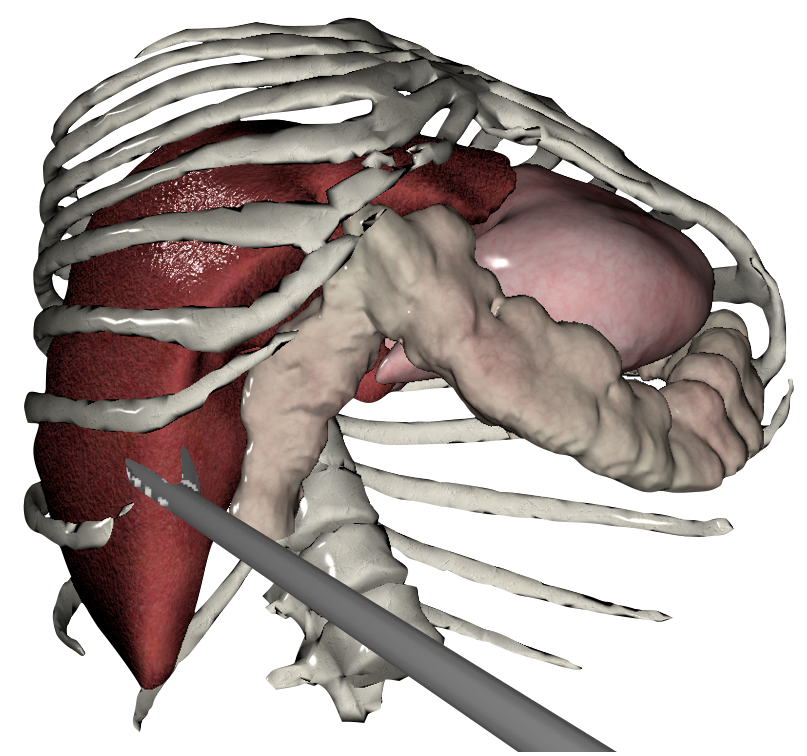
\includegraphics[width=0.48\linewidth]{NewLiver.png}
 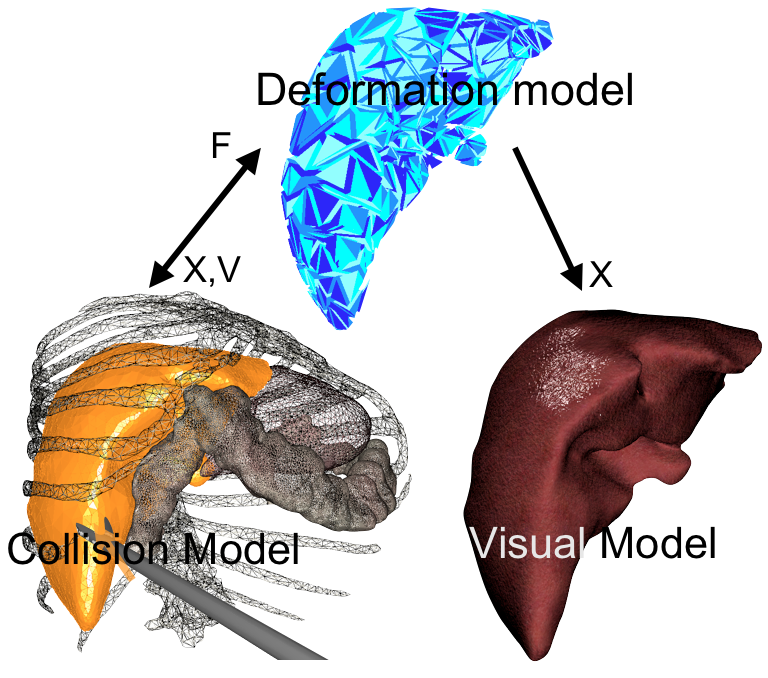
\includegraphics[width=0.5\linewidth]{NewLiverMap.png}
 \caption{A simulated Liver
Left: The simulation of the liver (dataset from IRCAD, France). Right: Three representations are used for the liver: one for the internal mechanics, one for the collisions, and one for the visualization.  These representations are linked using mappings (black arrows).}
 \label{fig:liver-multimodel}
\end{figure}

\section{Solid Mechanics} \label{sec:rigidAndDeformable}


Different models can be employed to discretize a deformable solid continuum as a dynamic or quasi-static system of particles (also called simulation nodes).
The node coordinates are the independent degrees of freedom (DOFs) of the object, and they are typically governed by equations of the following type:
% Some boundary conditions, composed of imposed motion at the node can be applied to the system.
\begin{equation}
 \label{eq:expliciteulerexample}
 \Va = \P \M^{-1} \sum_i \Vf_i (\Vx,\Vv)
\end{equation}
where \Vx and \Vv are the position and velocity vectors, the $\Vf_i$ are the different force functions (volume, surface and external forces in this example), \M is the mass matrix and \P is a projection matrix to  enforce boundary conditions on displacements. Note that the modeling of rigid body dynamics leads to the same type of equations.

The corresponding model in \sofa{} is a set of components connected to a common graph node, as shown in the right of Figure~\ref{fig:liver-mechanical}. 
%
\begin{figure}
 \centering
 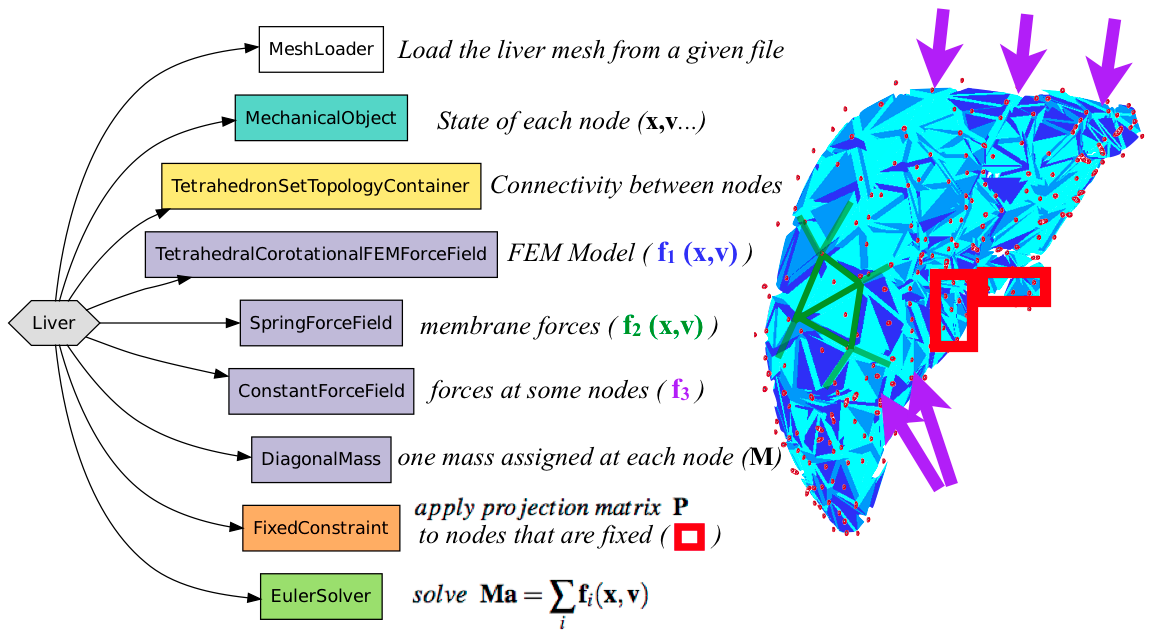
\includegraphics[width=0.95\linewidth]{liver-mechanical2.png}   % generated from ps using: dvipdf -dEPSCrop
 \caption{Mechanical model of a liver. In order to facilitate the combination of models and algorithms, the liver is described as a composition of specialized components.}
 \label{fig:liver-mechanical}
\end{figure}
%
Each component is responsible for a small number of tasks implemented using virtual functions in an object-oriented approach.
Each operator in Equation~\ref{eq:expliciteulerexample} corresponds to a component.
\textit{MeshLoader} is used to read the topology and the geometry.
The coordinate vector \Vx of the mesh nodes and all the other state vectors (velocity \Vv, net force $\sum \Vf$, etc.) are stored in \textit{MechanicalObject}, which is the core component of the mechanical model.
A tetrahedral connectivity is stored in \textit{TetrahedronSetTopologyContainer}, and made available to other components such as \textit{TetrahedralCorotationalFEMForceField}, which accumulates one of the terms of the force sum using the Finite Element method.
The two other terms come from \textit{SpringForceField}, which accumulates the forces generated by the membrane, and  \textit{ConstantForceField}, which accumulates external forces to a given subset of simulation nodes (for instance the pressure exerted by the diaphragm on the liver).
\textit{DiagonalMass} is used to implement the product with matrix $\M^{-1}$.
\textit{FixedConstraint} implements the product with matrix $\P$ to cancel the displacements of the squared particles.
\textit{EulerSolver} implements the logic of time integration.

This approach is highly modular because the components are completely independent of each other and are implemented using C++ classes with a reduced number of abstract functions. 
For instance, in the example of figure \ref{fig:liver-mechanical}, if one want to use a FEM for the membrane force instead of the spring based computation, only \textit{SpringForceField} has to be changed for \textit{TriangleFEMForceField}. Similarly, the mass matrix, stored as diagonal matrix in this example, can be stored as a single scalar value (\textit{UniformMass}) if less accuracy but faster computation is sought, in combination with an iterative solver for instance.



For efficiency, each mechanical state vector contains the values of all the simulation nodes, to avoid multiple call of virtual function resolutions.
The vector size is basically the number of particles times the number of space dimensions. 
We use C++ templates to avoid code redundancy between scalar types (float, double), the types of degrees of freedom (particles, frames, generalized coordinates), and the number of space dimensions.
All the particles in a vector have the same type known at compile time.
Degrees of freedom of different types must be grouped in different objects, possibly connected with interaction forces, as discussed in Section~\ref{sec:interactionforcefield}.
This greatly simplifies the design and allows aggressive compiler optimizations.

More than 30 classes of forces are implemented in SOFA, including springs, FEM for volumetric (tetrahedron or hexahedron) or surface (triangular shell and membrane) deformable objects using corotational or hyperelastic formulations, and for wire or tubular object (beam models meshed with segments), have been implemented.
Different types of springs allow for easy and fast modeling of the deformations (bending, compression/traction, volume, interactions between two bodies, joints...).
In rigid objects, the main components are the degrees of freedom (a single frame with 3 rotations and 3 translations) and the mass matrix that contains the inertia of the object. 
Surfaces can be attached to objects using \textit{mappings}, as discussed in Section~\ref{sec:mappings}.


\section{Collision models} \label{sec:collisionModels}
When a lot of primitives comes into contact, collision detection and response can become the bottleneck of a simulation. 
Several collision detection approaches have been implemented: distances between pairs of geometric primitives (triangles and spheres), points in distance fields, distances between colliding meshes using ray-tracing~\cite{HerFauRaf08}, and intersection volume using images~\cite{AFCFDK10}
The collision pipeline is described in section \ref{sec:collision} with more details. 

In order to adapt the models to the data structure of the different collision algorithms, we have defined a \textit{collision model}.
This model is similar to a mechanical model, except that its topology and its geometry are of its own and can be  stored in a data structure dedicated to collision detection. 
For instance, the component \textit{TriangleModel} is the interface for the computation of collision detection on a triangular mesh surfaces.

If the collision of a given simulation takes too much time, or to reduce the number of collision points, the meshes used for collision detection can be chosen less detailed than the mechanical ones. 
In the opposite, if precise collision detection and response is needed with  smooth surfaces, it is sometimes suitable to use more detailed mesh for collision detection.











%%%%%%%%%%%%%%%%%%%%%%%%%%%%%%%
\section{Visual models} \label{sec:visual}

In the context of surgical simulation for training, to reach the state of what is often called \textit{suspension of disbelief} i.e. when the user forgets that he or she is dealing with a simulator, there are other factors than the mechanical behavior. 
Realistic rendering is one of them. 
It involves visually recreating the operating field with as much detail as possible, as well as reproducing visual effects such as bleeding, smoke, lens deformation, etc.
The main feature of the visual model of SOFA is that the meshes used for the visualization can be disconnected from the models used for the simulation. 
The mappings described in section \ref{sec:mappings} maintain the coherency between them.
Hence, SOFA simulation results can easily be displayed using models much more detailed than used for internal mechanics, and rendered using external libraries such as OGRE\footnote{www.ogre3d.org} and Open Scene Graph\footnote{www.openscenegraph.org}.

We have also implemented our own rendering library based on openGL. 
This library allows for modeling and render the visual effects that occurs during an intervention or the images that the surgeon is watching during the procedure.
For instance, in the context of interventional radiology simulator, we have developed  a dedicated interactive rendering of X-ray and fluoroscopic images. 





 \section{Mappings} \label{sec:mappings}
As previously discussed, objects simulated in \sofa, like the liver in Figure \ref{fig:liver-multimodel}, typically rely on several models: one for the internal model, one for collision, and one for the visual rendering. 
To enforce consistency, one of them, typically the internal model, acting as the master, imposes its displacements to slaves (typically the visual model and the collision model), using \textit{mappings}.
Mapped model can be masters of other models in turn, creating a hierarchy whith the independent DOFs at the root.
Figure \ref{fig:hierarchy} illustrates the hierarchies of two objects. The visual models, in additional branches, are omitted for clarity. When contact models collide, additional geometry is necessary to model the contacting points.
This additional geometry is represented in an additional level connected to the models, as depicted in the figure. 


The positions $\vec x_c$ of a child model are computed by the mapping based on the positions $\vec x_p$ of the master using a function $\JNL$. 
\begin{equation} %\label{eq:mapV}
\vec x_c =\JNL(\vec x_p)
\end{equation}
% In the particular case of a FEM model, this mapping function can rely on the underlying interpolation of the model. 
% 
% 
% These mapping are implemented in a very generic way and allows the control of any kind of slave model $\vec x_1 = \JNL_1(\vec x_0)$ given the position of a master model $\vec x_0$ . 
The velocities can be mapped in a similar way:
\begin{equation}
\vec v_c = \mat J \vec v_p
\end{equation}
The Jacobian matrix $\mat J = \frac{\partial \vec x_c}{\partial \vec x_p}$ encodes the linear relation between the parent and child velocities.
It also holds on accelerations, with an additional offset due to velocities when the position mapping $\JNL$ is nonlinear.
In linear mappings, operators $\JNL$ and $\J$ are the same, otherwise $\JNL$ is nonlinear with respect to $x_p$ and it can not be written as a matrix.
For surfaces embedded in deformable cells, matrix $\J$~contains the barycentric coordinates (it corresponds to linear interpolation in FEM).
For surfaces attached to rigid bodies, each row of the matrix encodes the usual relation $v = \dot o + \omega \times (x-o)$ for each vertex. 

The positions and the velocities are propagated top-down in the hierarchy. 
Conversely, the forces are propagated bottom-up, up to the independent DOFs, where Newton's law $\vec f=\M\vec a$ is applied. 
Given forces $\vec f_c$ applied to a child model, the mapping computes and accumulates the equivalent forces $\vec f_p$ applied to its parent. 
Since equivalent forces must have the same power, the following relation holds:
$$
\vec v_{p}^T \vec f_p = \vec v_c^T \vec f_c
$$
The kinematic relation $\vec v_{c} = \J \vec v_{p}$ allows us to rewrite the previous equation as
$$
\vec v_{p}^T \vec f_{p} = \vec v_{p}^T \J^T \vec f_c
$$
Since this relation holds for all velocities $\vec v_p$, the principle of virtual work allows us to simplify the previous equation to obtain:
\begin{equation} \label{eq:mapF}
\vec f_{p} = \J^T \vec f_c
\end{equation}
When a model has several children, each child accumulates its contribution to the parent forces using its mapping. 
This hierarchical kinematic model allows us to compute displacements and to apply forces at all levels.
%
\begin{figure}
 \centering
 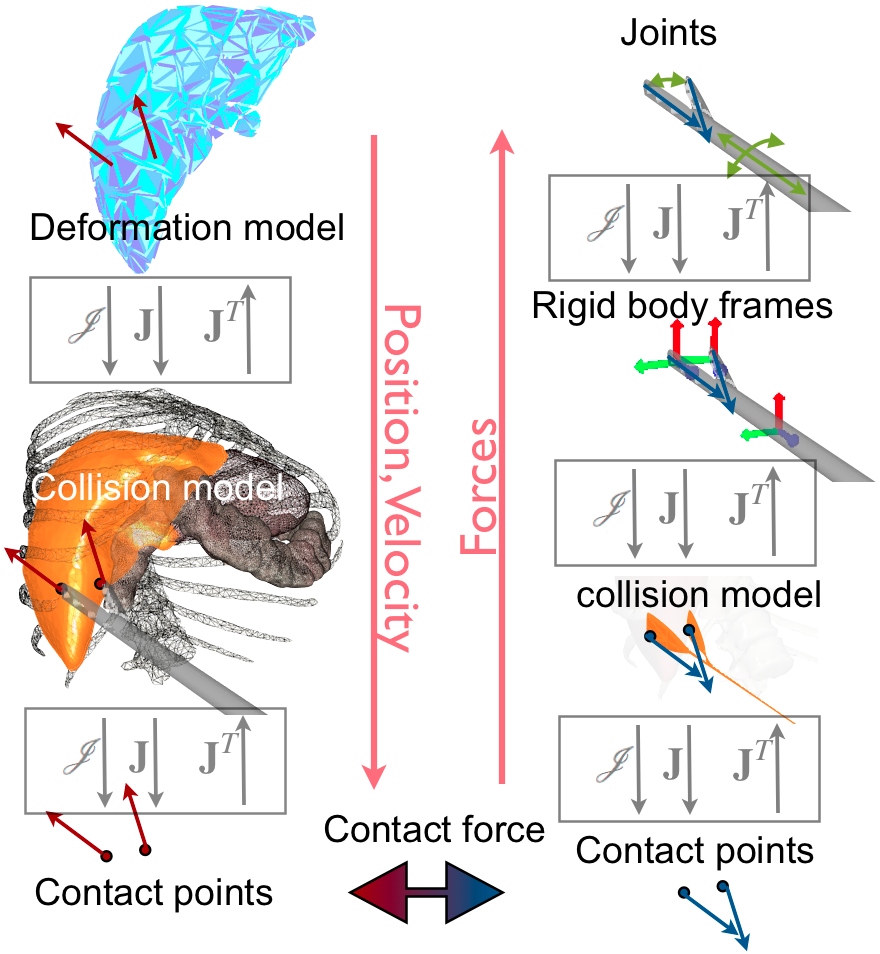
\includegraphics[width=0.9\linewidth]{MappingScheme.png}
 \caption{Mappings from the DOFs to the contact point. Right (top to bottom): The Mechanical model of the liver is based on Finite Element model. A triangular mesh is mapped for collision detection with the surface. The two contact points found by the collision detection (with the grasper) are mapped on the collision model. 
 Left (bottom to top): the contact points are also mapped on the collision model of the grasper. This collision model is a simplification of the grasper shape and is mapped on the rigid body frames. The motion of these frame is mapped on the state of the joints which are the independent DOFs of the grasper.
}
 \label{fig:hierarchy}
\end{figure}
%
So far, $22$ variants of mappings have been implemented to attach models to rigid objects and deformable primitives such as tetrahedra, hexahedral grids, splines, blended frames, flexible beams and scalar fields.
Mappings are also be used to connect generalized coordinates, such as joint angles, to world-space geometry, as in the grasper of Figure~\ref{fig:hierarchy}.


%% attacher de la g�om�trie
%
%
%They are not independent variables, since the positions and velocities are bound to the independent DOF.
%We say that a child geometrical model $1$ is \textit{mapped} from its parent model $0$,
% using a kinematic operator which we call \textit{mapping}. It implements the kinematic relations:
%\begin{eqnarray*} %\label{eq:mapV}
%\vec x_1 &=&\JNL_1(\vec x_0)\\ 
%\vec v_1 &=& \mat J_1 \vec v_0
%\end{eqnarray*}
%Mappings allow to attach polygonal shapes (like the tool shape in Figure~\ref{fig:hierarchy}, with point DOFs) to rigid bodies (with frame DOFs) using local coordinates, or to embed the shapes in deformable cells using barycentric coordinates (like the deformable liver in Figure~\ref{fig:hierarchy}), among other possibilities.
%Matrix $\mat J_1 = \frac{\partial \vec x_1}{\partial \vec x_0}$ encodes the linear relation between the parent and child velocities.
%It also holds on accelerations, with an additional offset due to velocities when the position mapping \JNL is nonlinear.
%In linear mappings, operators \JNL and \J are the same, otherwise \JNL is nonlinear with respect to $x_0$ and it can not be written as a matrix.
%For surfaces embedded in deformable cells, matrix \J~contains the barycentric coordinates. 
%For surfaces attached to rigid bodies, each row of the matrix encodes the usual relation $v = \dot o + \omega \times (x-o)$ for each vertex. 
%% Similarly, skins around articulated bodies involve, at each vertex, the weighted  contributions of the rigid bodies. 


%% g�om�trie suppl�mentaire d�e aux contacts
%When shapes collide, additional geometry is necessary to model the contact.
%For instance, when an edge intersects or closely approaches another one, a contact force is typically applied to the intersection point or to the pair of points.
%The points are defined using their barycentric coordinates with respect to the edge vertices. 
%% Other relations can be used, depending on the kind of geometrical primitives in contact.
%This additional geometry can be represented in another geometrical layer connected to the shape by a mapping, as illustrated in the bottom of Figure~\ref{fig:hierarchy}.
%% This layer is also connected to the shape using mappings:
%% \begin{eqnarray*} %\label{eq:mapV}
%% x_2 &=&\JNL_2(x_1)\\ 
%% v_2 &=&J_2 v_1 
%% \end{eqnarray*}
%
%We generalize this approach to tree-like hierarchies of geometries, with the independent DOFs at the root. 
%For instance, the independent DOFs may have two children, one for collision using a coarse mesh, and the other for rendering using a finer mesh.
%The hierarchy have more levels, for instance, to attach collision spheres to a mesh embedded in a deformable grid. 
%The synchronization between these models is automatically guaranteed by their attachment to their common ancestor, using graph visitors as explained in Section~\ref{sec:visitors}.
%Positions and velocities are propagated top-down in the hierarchy. Conversely, the forces are propagated bottom-up, up to the independent DOFs, where Newton's law $f=ma$ is applied. 
%Given forces $f_c$ applied to a child model, the mapping computes and accumulates the equivalent forces $\vec f_p$ applied to its parent. 
%Since equivalent forces must have the same power, the following relation holds:


% In implicit simulation methods, one needs to consider force changes $\vec{df}$ corresponding to small displacements $\vec{dx}$ of the independent DOF.
% This involves the forces applied to the independent DOF, but also the forces are applied to mapped DOFs.
% Let $0$ denote the independent DOF.%, and $n$ a level mapped through $n$ mappings indexed from $0,1$ to $n-1,n$.
% At each hierarchy node $i$, let $\mat K_{ii}$ be the stiffness matrix corresponding to the forces applied to the local DOF.
% The local displacement is :
% \begin{equation} \label{eq:displacementsTopDown}
%  \vec{dx}_{i} = \prod_{j=1}^{i}\mat J_{j,j-1} \vec{dx}_{0}
% \end{equation}
% where $\prod_{j=1}^{i}\mat J_{j,j-1} = \mat J_{i,i-1}...\mat J_{1,0}$ is the product of the matrices of the mappings in the path from the independent DOF to node $i$.
% The matrix-vector product can be efficiently computed during one top-down traversal of the hierarchy, with one matrix-vector product at each level, without any matrix-matrix product.
% Conversely, the resulting force change on the independent DOFs is:
% \begin{equation} \label{eq:forcesBottomUp}
%  \vec{df}_{0} = \left( \prod_{j=1}^{i}\mat J_{j,j-1} \right)^T \vec{df}_{i}
% \end{equation}
% where $\left( \prod_{j=1}^{i}\mat J_{j,j-1} \right)^T = \mat J_{1,0}^T...\mat J_{i,i-1}^T$ is the product of the transposed matrices of the mappings in the path from node $i$ to the independent DOF.
% This matrix-vector product can be efficiently computed using matrix-vector products during one bottom-up traversal of the hierarchy.

%Figure~\ref{fig:liver-mechanical-spheres} shows a sphere-based collision model attached to the mechanical model of Figure~\ref{fig:liver-mechanical}. 
%The position vector of the collision model is the set of 3d coordinates of the sphere centers, defined by their barycentric coordinates stored in the BarycentricMapping.
%\begin{figure}
% \centering
% 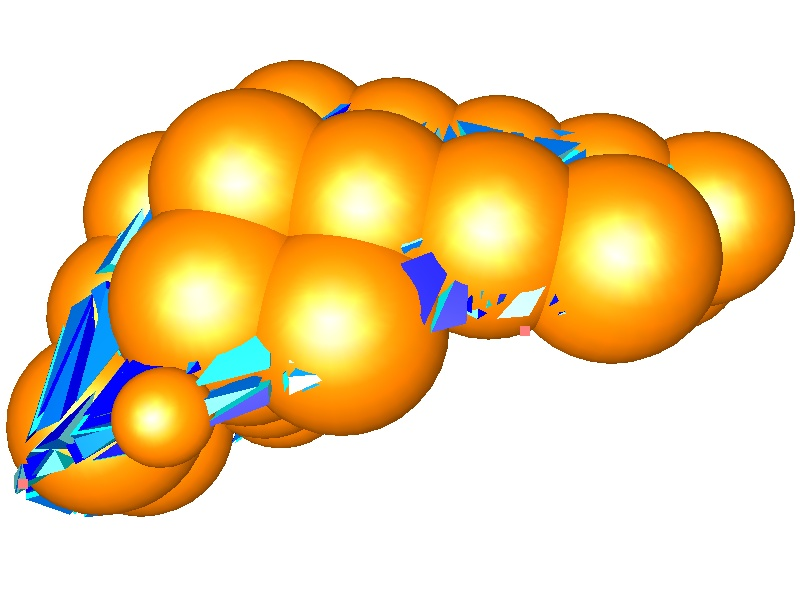
\includegraphics[width=0.4\linewidth]{liver-spheres-superimposed.jpg}
% 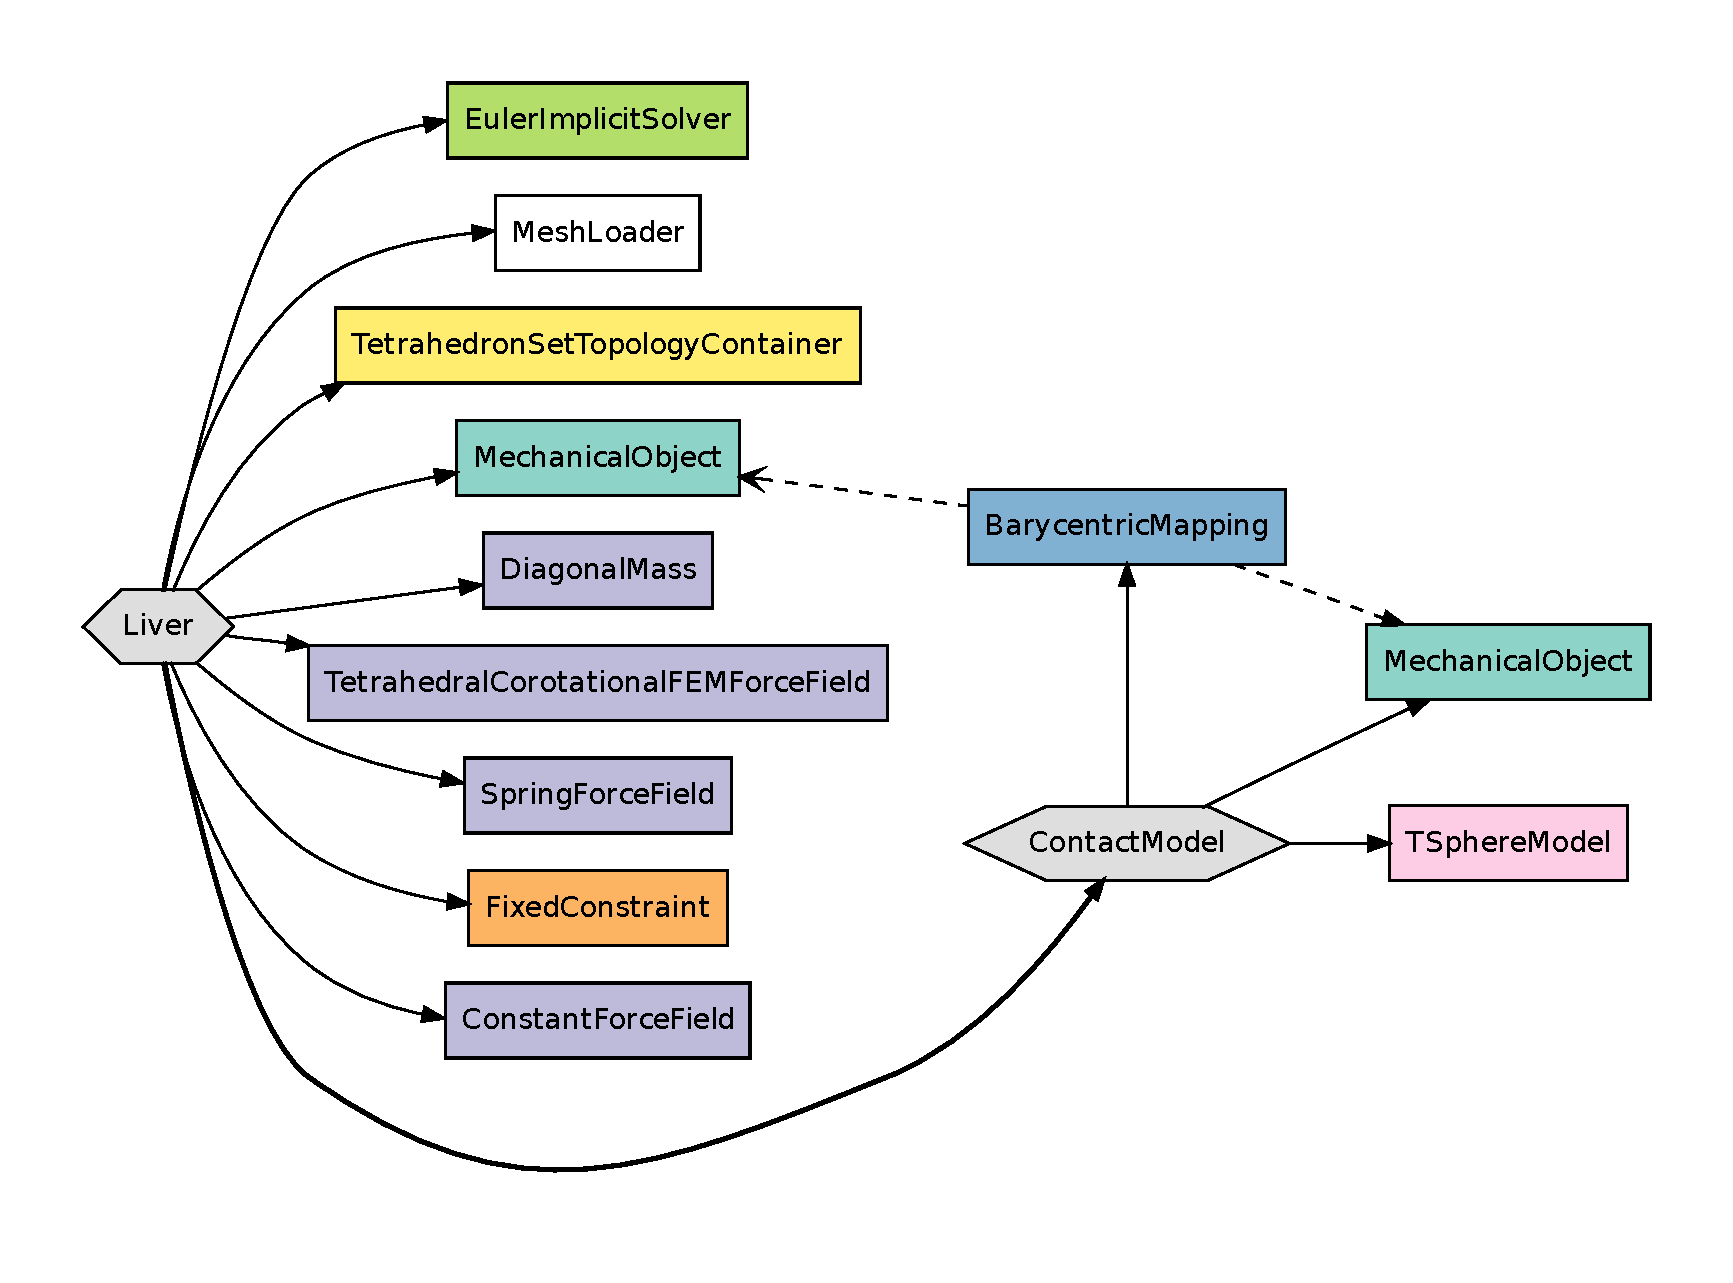
\includegraphics[width=0.56\linewidth]{liver-spheres.pdf}   % generated from ps using: dvipdf -dEPSCrop
% \caption{Left: mechanical (in blue) and collision (in yellow) models of a liver. Right: the corresponding scene graph. The plain arrows denote hierarchy, while the stippled arrows represent connections.}
% \label{fig:liver-mechanical-spheres}
%\end{figure}







\chapter{Data Structure}
The organization of simulation data is a complex issue. We have identified three relevant levels, and proposed different solutions for each of them.
The coarsest structure is the scenegraph, used to hierarchically organize the groups of objects and their multi-models.
At a finer scale, the attributes of the components can be linked by relations.
Finally, the geometrical models and the topological changes deserve a special attention.
\graphicspath{{../datastructure/}}  % to include images
\section{Scene-Graph}
% \subsection{Multiple objects}\label{sec:multiple}
When the simulation involves several objects, we model them as different branches in a scenegraph data structure.
In the example shown in Figure~\ref{fig:twoObjects}, the scene contains two objects animated using different time integrators, collision detection components (discussed in Section~\ref{sec:collision}), an interaction force, and a camera to display the objects.
The root node does not contain DOFs.
It is used to contain the components which are common to its child nodes.
\begin{figure}
 \begin{center}
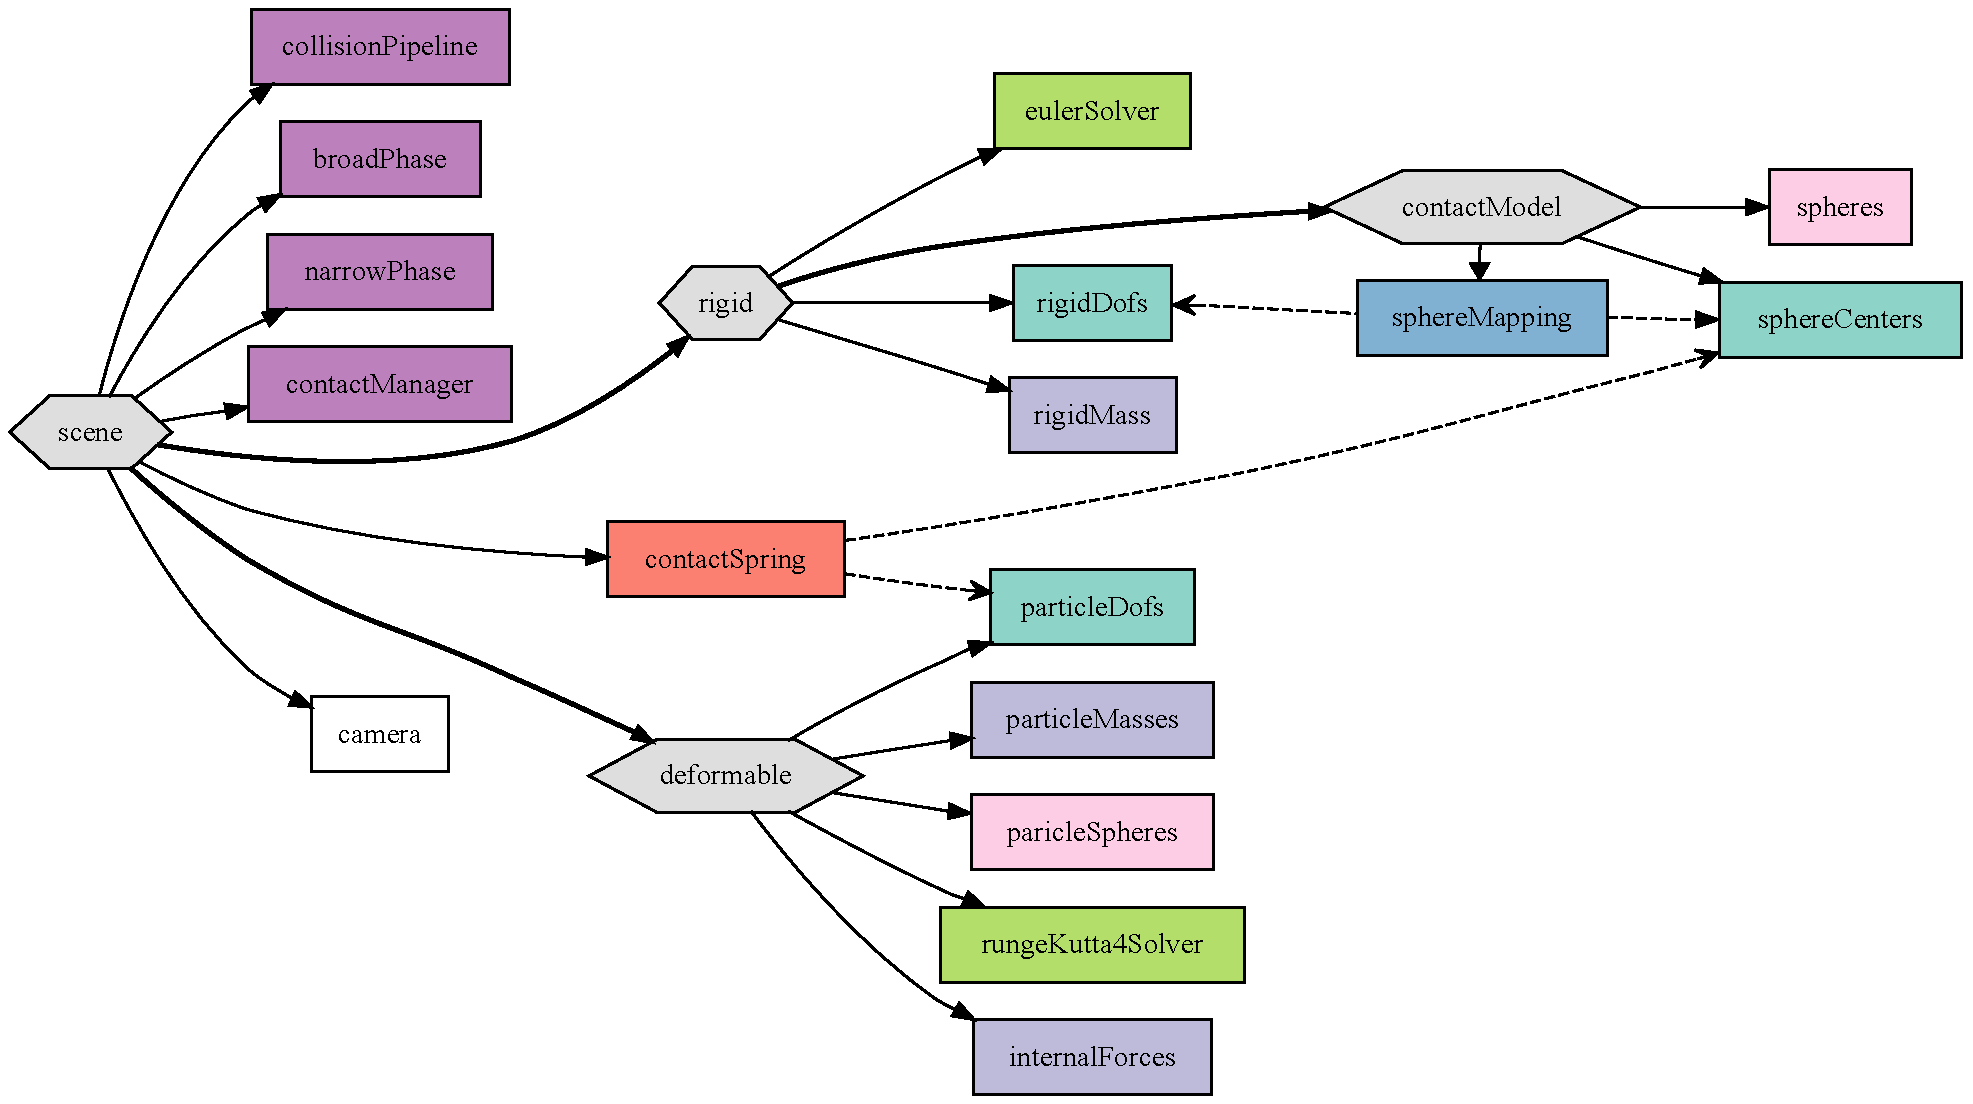
\includegraphics[width=0.98\linewidth]{twoObjects.pdf}
 \caption{A scenegraph with collision detection and two independent objects interacting through a spring.}                                                                      
 \label{fig:twoObjects}
\end{center}
\end{figure}
% Applying the same ODE solver to all the objects is as simple as attaching the corresponding component to the common ancestor node.
% This allows to process the objects and their interaction forces in a common equation system, which is necessary when stiff interaction forces or Lagrange multipliers are used for coupling the objects. 
% When each object has its own solver, the interaction force is considered constant during the time step.

Scenegraphs are popular in Computer Graphics due to their versatility.
The data structure is processed using visitors (discussed in Section~\ref{sec:visitors}) which apply virtual functions to each node they traverse, which in turn apply virtual functions to the components they contain.
% , and the visitor-based approach presented in Section~\ref{sec:visitors} allows us to apply operations to all the branches, possibly in parallel. 
In basic scenegraph frameworks, the visitors are exclusively fired from an external control structure such as the main loop of the application.
In \sofa, the components are allowed to suspend the current traversal to send an arbitrary number of other visitors, then to resume or to prune the suspended visitor.
This allows us to implement global algorithms (typically ODE solution or collision detection), such as the explicit Euler velocity update of Equation~\ref{eq:expliciteulerexample}, in components.
This neatly decouples the physical model from the simulation algorithms, in sharp contrast with dataflow graphs which intricate data and operators in the same graph.
Replacing a time integrator requires the replacement of one component in our scenegraph, whereas the corresponding dataflow graph would have to be completely rewritten.




Interactions between objects may be handled using penalty forces or Lagrange multipliers. 
In all cases, a component connected to the two objects is necessary to geometrically model the contact and compute the interaction forces.
This component being shared between the two objects, it is located in their common ancestor node.
The coupling created by penalty forces should be seen as soft or stiff, depending on the stiffness and the size of time step~\cite{baraff98large}.
A soft coupling can be modeled by an interaction force constant during each time step.
In this case, each object can be animated using its own, possibly different, ODE solver.
% The interaction force is computed and accumulated  when the AnimateVisitor traverses the ancestor nodes before reaching each solver in their child branches.
% This ensures that the object undergo opposite interaction forces during the time step, but it requires the synchronization of the object at the end of each time step.
% Animating the two objects at different time steps would be possible, using each solver independently instead of a common AnimateVisitor, but this would require an additional mechanism to update the interaction and enforce Newton's third law on opposite forces.
The assumption of constant interaction force during each time step is compatible with all explicit time integration methods.
However, when the interaction forces are stiff, implicit integration is necessary to apply large time steps without instabilities.
This requires the solution of an equation system involving the two objects as well as their interaction force together.
In this case, the ODE solver is placed in the common ancestor node, at the same level as the interaction component.
This is also true for constraint-based interaction which requires the computation of Lagrange multipliers based on interaction Jacobians. 
% \todo{illustrer sur une figure}
% We call it \textit{hard coupling} when the interacting objects and the interaction forces need to be solved simultaneously in a common equation system.
% This includes stiff penalty forces and Lagrange multipliers.
Due to the superlinear time complexity of equation solvers, it is generally more efficient to process independent interaction groups using separated solvers rather than a unique solver.

% 
% Contact interactions created during the simulation may be soft, stiff of constraint-based, depending on the collision response stategy, as explained in Section~\ref{sec:collision}.
% In case of hard coupling, a group manager is used to gather objects in the smallest possible groups.


% \subsubsection{The context} \label{sec:components}
% \SC{I would remove this subsection - it is redundant with some of the other text}
% 
% % \todo{Description plus détaillée des composants : principe de séparation des données (State,TopoContainer), des calculs (FF,TopoModifier,...), et des dépendances (Node)}
% % 
% % \todo{Présentation de l'utilisation des templates : comment ils permettent dans les composants d'avoir des codes génériques tout en étant instancié et optimisé par le compilateurs pour chaque type de DOF.}
% All the components acting on the same DOFs are gathered in a common node, which main contain: 
% % A node may represent a set of physical objects, such as the root of the scene or a collision group, using the list of child nodes.
% % Groups may contain algorithm components, applied to all the children using graph visitors as explained in Section~\ref{sec:visitors}. 
% % These include ODE solvers to integrate time, collision detection algorithms, and MasterSolvers to schedule the formers.
% % Groups may also include components associated with interactions between the child nodes, as discussed in Section~\ref{sec:interactions}.
% % A node may also represent one kinematic layer of a physical object, i.e. a set of components associated with the same degrees of freedom.
% % This includes: 
% \begin{itemize}
%  \item a container of state vectors, to represent coordinates, velocities, forces, accelerations and any auxiliary vector used by the algorithms. Each state vector contains the values associated to all the nodes. All the following components in this list read and write the state vectors in this component.
%  \item a list of topology containers, to model mesh edges, faces and cells based on node indices.
%  \item a mass, to compute accelerations based on forces, and momentums based on velocities.
%  \item a list of force functions, to accumulate forces based on positions and velocities. They can be used to model internal or external forces, including force boundary conditions.
%  \item a list of projective constraints, to filter the state vectors to cancel forbidden displacements. They can be used to apply displacement boundary conditions to each indendent DOF.
%  \item lists of geometrical primitives used in collision detection.
%  \item a list of child nodes, to create hierarchies and complex scenes (see sections~\ref{sec:mappings} and \ref{sec:scenes})
%  \item a mapping, to synchronize the local DOFs with master DOFs higher in the hierarchy
%  \item a list of constraints to handle using Lagrange multipliers, more complex but more general than projective constraints. They can be used to apply constraints to non-independent DOFs.
%  \item lists of components implementing algorithms for collision detection(\ref{sec:collision}) and the solution of equations (section~\ref{sec:odesolvers})
% \end{itemize}
% While most of the data is private, some is available to all the components, especially the topology and the state vectors. 
% % These attributes are used by the visitors to access the components during the graph traversals.
% % The connections between the components attached to the same node are generally implicit, because there is a unique container of state vector and a unique topology, which allows the components to find the necessary data.
% For instance, 
% % a TetrahedronFEMForceField computes viscoelastic forces based on the deformation of tetrahedra. 
% the list of tetrahedra used by a TetrahedralFEMForceField is stored in the local topology container, while the initial and current particle states are stored in the MechanicalObject. 
% The same list of tetrahedra may be used to define the embedding of auxiliary DOFs in children nodes, as discussed in Section~\ref{sec:mappings}.
% % Additionally, nodes contain lists of control components to implement simulation algorithms, such as EulerSolver, as discussed in Section~\ref{sec:control}.



\subsection*{Visitors} \label{sec:visitors}
% The top-down and bottom-up force computation presented in Section~\ref{sec:mappings} is easily generalized to an arbitrarily branched hierarchy with forces applied at all levels.
We implement the simulation using visitors which traverse the scene top-down and bottom-up, and call the corresponding virtual functions at each graph node traversal. 
A possible implementation of the traversal of a tree-like graph is shown in the left of Figure~\ref{fig:visitorTraversal}.
Algorithmic operations on the simulated objects are implemented by deriving the Visitor class and overloading its virtual functions \textit{topDown(~)} and \textit{bottomUp(~)}. 
This approach hides the scene structure (parent, children) from the components, for more implementation flexibility and a better control of the execution model.
The data structure can easily be generalized from strict hierarchies to directed acyclic graphs for more general kinematic dependencies.
Moreover, various parallelism strategies can be applied independently of the mechanical computations performed at each node.
\begin{figure}
\begin{center}
\begin{tabular}{l|r}
\begin{minipage}{0.4\linewidth}
\begin{algorithmic}
\STATE void  \textbf{Visitor::traverse(Node n)}
\STATE bool continue = this.topDown( n )
\IF{continue} 
\FORALL {c child of n} 
\STATE traverse( c ) 
\ENDFOR
\STATE     this.bottomUp( n )
\ENDIF
\end{algorithmic} 
\end{minipage}
 &
\begin{minipage}{0.5\linewidth}
\begin{algorithmic}
% \renewcommand{\algorithmicendfor}{}
% \renewcommand{\algorithmicendif}{}
\STATE bool  \textbf{AnimateVisitor::topDown(Node n)}
\IF{masterSolver} 
\STATE masterSolver.animate(this.dt)
\RETURN false
\ENDIF
\IF{collisionPipeline} 
\STATE collisionPipeline.modelContacts()
\ENDIF
\IF{odeSolver} 
\STATE odeSolver.solve(this.dt)
\RETURN false
\ENDIF
\FORALL {InteractionForce f}
\STATE f.apply()
\ENDFOR
\RETURN true
\end{algorithmic} 
\end{minipage}
\end{tabular}
\end{center}
\caption{Left: a recursive implementation of the visitor traversal. Right: the AnimateVisitor. }
\label{fig:visitorTraversal}
\end{figure}

Forward time stepping is implemented using the \textit{AnimateVisitor} traversal method, shown in the right of Figure~\ref{fig:visitorTraversal}.
Applied to the simple scene in Figure~\ref{fig:liver-mechanical-spheres}, it triggers the ODE solver, which in turn applies its algorithm using visitors for mechanical operations such as propagating states through the mappings or accumulating forces.
Note that the traversal of the AnimateVisitor is pruned when a ODE solver is encountered.
This allows the ODE solver to take control of its subgraph and to overload lower-level solvers, which are not reached by the AnimateVisitor.
In the more complex scene shown in Figure~\ref{fig:twoObjects}, the solver triggers the collision detection, which may create a contact between the chidren, such as contactSpring.
The visitor then triggers the computation of the interaction force, which will be seen by the objects as a constant, external force during the time step.
The visitor then continues the traversal and triggers each object ODE solver.
The default behavior is to model the contacts prior to applying time integration.
To implement other strategies, a \textit{MasterSolve}r can be used to prune the visitor and apply time integration and collision detection in a different order, possibly looping until all collisions are solved.

\begin{figure}
 \centering
 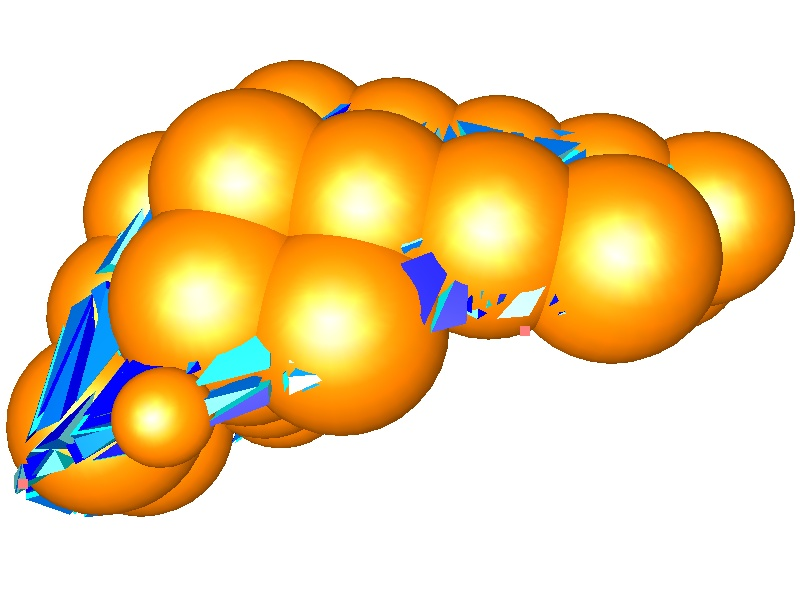
\includegraphics[width=0.4\linewidth]{liver-spheres-superimposed.jpg}
 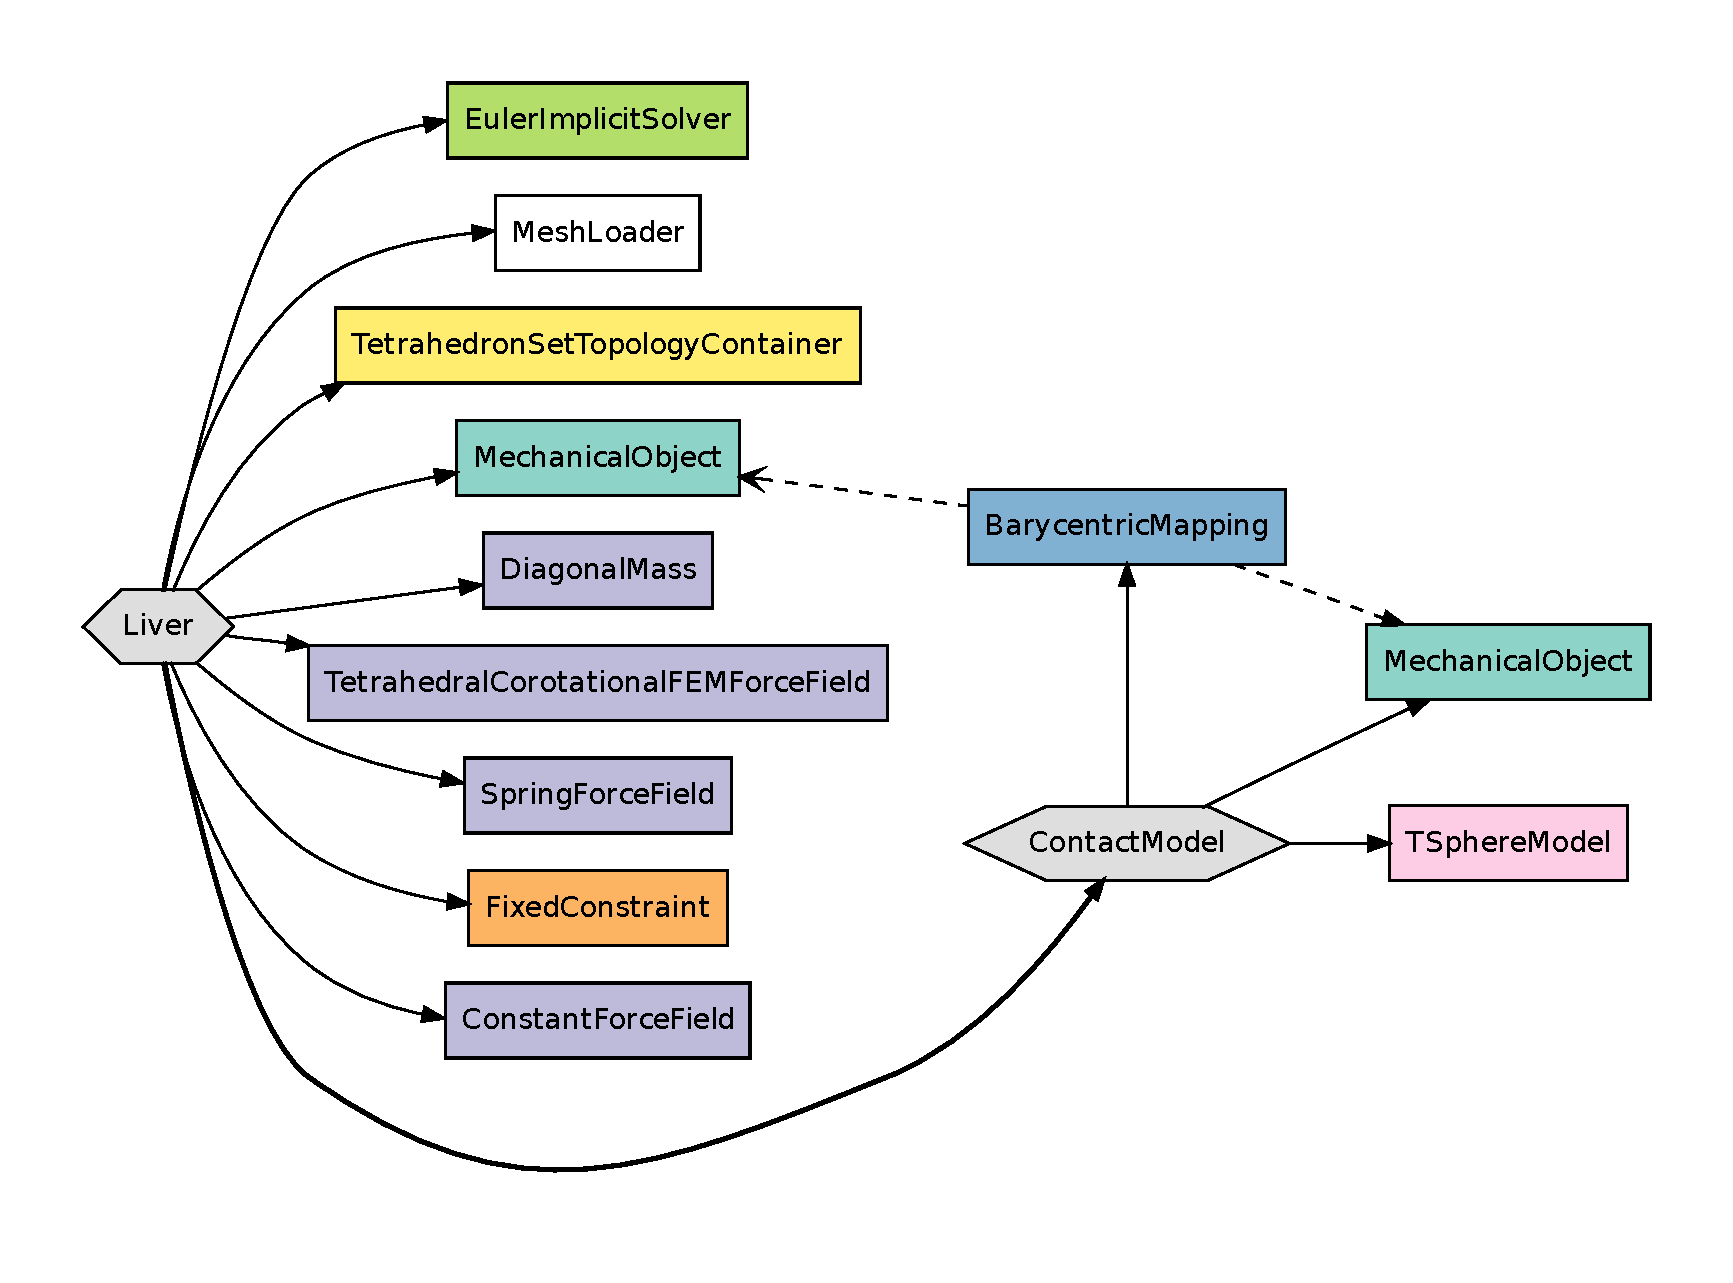
\includegraphics[width=0.56\linewidth]{liver-spheres.pdf}   % generated from ps using: dvipdf -dEPSCrop
 \caption{Left: simple mechanical (in blue) and collision (in yellow) models of a liver. Right: the corresponding scene graph. The plain arrows denote hierarchy, while the stippled arrows represent connections.}
 \label{fig:liver-mechanical-spheres}
\end{figure}


\section{Data, Engines and Tags}

Component parameters are stored in member objects using \textit{Data} containers, templated on the type of attribute they represent.
For instance, the list of particle indices constrained by a FixedConstraint is stored in a \lstinline!Data< vector<unsigned> >!.
These containers provides a reflective API, used for serialization in XML files and the automatic creation of input/output widgets in the user interface, as discussed in Section~\ref{sec:interface}.
% When the same data is needed by different components, each component contains a corresponding Data object, and these Data are synchronized using connections.
%This eases thread-safe programming \SC{true ?} and allows the automatic computation and the update of Data dependencies using operator objects called \textit{Engines}.
We can create connection between Data instances to keep their value synchronized. This is used for instance when a \textit{Loader} component loads several attributes from a file (such as topology, positions, stiffnesses, boundary conditions) which are then connected to one or more components using it as input.
In some cases we need to not simply copy an existing value but compute it from one or several Data. This feature is provided by \textit{Engine} components.
%We can also create connections through an \textit{Engine}, which is used when 
Engines contain input and output Data, and their update method computes the output based on the input.
%When a Data value is changed, the connected Data are flagged as \textit{dirty}, and so on recursively through connections and engine input-outputs.
A mechanism of lazy evaluation is used to recursively flag Data values that are not up-to-date, but they are recomputed only when necessary.
For instance, based on a bounding box and a vector of coordinates, a BoxROI engine computes the list of indices of the coordinates inside the box. These indices can then be used as input of a FixedConstraint to define a fixed boundary condition. With this design, the simulation can transparently be setup either from data stored in static files, or generated automatically with engines.

The network of interconnected Data objects defines a data dependency graph, superimposed on the scene graph.
This two-graph framework is used in other graphics software such as OpenInventor and Maya, where engines are used to generate the animation, by periodically updating the state vectors using time as input. 
However, while this approach works well for straightforward computation pipelines, such as keyframe interpolation, it does not easily allow the branching and loops control structures used in sophisticated physical simulation algorithms.
It is also a rather low-level representation, essentially encoding every computation steps required to compute a given Data.
Consequently, we only use Engines to implement straightforward relations between the parameters of the model, which may remain unchanged during the simulation.
% \SC{ True? Could we really not use this mechanism instead of mappings? It  would be nice to explain the difference with the mappings ;-)}
In \sofa{}, the state update algorithms are instead determined by combining several components, communicating through scenegraph visitors, as explained in Section~\ref{sec:solvers}.

\subsection*{Objects and node tagging (\textcode{Tag} and \textcode{TagSet}).}

The goal of the introduction of tags is to provide one of the pieces necessary to support non-mechanical states (electrical potentials, constrast agent concentrations) as well as cleaner non-geometrical mechanical states (fluid dynamics, reduced-coordinate articulations).
For example, in a simulation involving blood in deformable vessels, we would use two tags to distinguish the different states : mechanical, fluid.
These tags will be used to easily work with only a subset of the components, so that the mechanical solver works on positions and forcefields but don't interferes with blood flow and pressure, and inversely for the fluid solver (see \footnote{http://wiki.sofa-framework.org/tdev/wiki/Notes/ProposalGenericStates} ).
We decided on using there tags instead of extending the class hierarchy as was done before with the \textcode{State} and \textcode{MechanicalState} classes.
A hierarchy is fine when we have only one feature that we want to differentiate on (such as base vs mechanical vs electrical), but when we add other criteria (lagrangian geometry vs eulerian vs reduced generalized coordinates, velocity vs vorticity, independent vs mapped DOFs) it is no longer manageable as specialized classes.
A secondary use of these tags is to replace existing subsets mechanisms within CollisionModels (r2441) and Constraints (r3121).
The design is based on the following elements.
Tags are added to BaseObject, as a list of string (internally converted to a list of unique ids for faster processing).
All visitors now filter the objects they process based on their list of tags.
All solvers by default copy their own list of tags to the visitors they execute, so that they only affect the objects with the same tags as they have (TODO: this is currently broken). 

\newpage
\section{How to use mesh topologies in SOFA}

H. Delingette, B. Andr�

\subsection{Introduction}

\subsubsection{BTW, What is a mesh topology ?}

A mesh is usually described as a set of points that are connected by
edges, triangles or any other type of mesh element. Thus it is
useful to make a clear a distinction between two different aspects
of a mesh :

\begin{itemize}

 \item \textbf{Mesh Geometry} : the mesh geometry consists in the position of the mesh vertices.
This information depends on the space where the mesh in embedded.
For instance in a 2D triangulation, each vertex position is a 2D
vector while in a 3D triangulation, each vertex position is a 3D
vector. Therefore the mesh geometry can be described as an array of
vector whose size is the number of mesh vertices. In SOFA, we use
the word Degree Of Freedom (DOF) to describe such an array because
it can be used to store other geometric information (rigid
transformation, first or second derivatives, etc.).

 \item \textbf{Mesh Topology} : the mesh topology describes how the vertices are
connected with each other. For instance, it describes the set of
triangles by specifying the 3 vertex indices that make each
triangle. A mesh topology manipulates vertex indices (as unsigned
int) and therefore is independent of the embedding space. For
instance, a 2D and a 3D triangulation may have the same mesh
topology but with different mesh geometry.

\end{itemize}


\subsubsection{Why do I need to bother with mesh topologies ?}

As discuss above, mesh topology is an essential part of a mesh and
therefore any computation task that requires a mesh needs to know
how to use a mesh topology.\\ This includes:

\begin{itemize}

 \item \textbf{Mesh Visualization},

 \item \textbf{Collision detection} : some collision detection are mesh based (e.g.
triangles or edges),

 \item \textbf{Mechanical Modeling} : deforming a mesh also requires to the
knowledge of a mesh topology. For instance a spring mass model
requires knowing about the edges that connects pair of vertices,

 \item \textbf{Haptic rendering},

 \item \textbf{Description of scalar} (temperature, electric potential, etc.) or
vectorial fields (speed, fiber orientation, etc.)

\end{itemize}

Using a mesh topology is relatively simple since it consists in
having access to arrays of indices corresponding to vertex indices
or edge indices or other topological items.
\\

A more tricky part consists a) in changing locally or globally this
topology (adding a triangle, removing an edge) and b) in propagating
those changes to all objects using the mesh topology to perform a
task (visualization, deformation, etc.)

\subsubsection{How are Mesh Topologies designed in SOFA ?}

The mesh geometry in SOFA is stored in a MechanicalObject which is a
template class because it depends on the embedding space (2D or 3D
Euclidian space), the vector class and the required floating point
accuracy (float vs double).
\\

A mesh topology is stored in a different object than the mesh
geometry.
\\

One important aspect of the design of mesh topologies in SOFA is the
fact that they are organized in a class hierarchy. For instance, a
triangulation object derives from an edge set object since a
triangulation can be also viewed as a set of edges, each triangle
having 3 edges. This is very important to design generic software
components. Indeed, following the same example, with this design, a
spring mass mechanical model that only requires the knowledge of
edges (pairs of vertices) can also be used on a triangulation or any
other mesh (quad, hexahedral, tetrahedral mesh)  that derives from
an edge set object.
\\

Another interesting feature in SOFA is the ability to provide
multiple topology descriptions for the same mesh. For instance a
quad element (see figure below) has four DOFs which can be connected
with 2 triangles or 6 edges. Thus, the same mesh geometry can be
described by 3 different mesh topologies. SOFA uses the mechanism of
topological mapping to provide multiple topologies associated with
the same mesh geometry. Those mappings also apply to map a subset of
the mesh topology into a new mesh topology.  For instance the border
of a tetrahedral mesh can be mapped into triangulation mesh or edges
of a triangulated mesh can be mapped into a polygonal mesh.\\


\begin{figure*}
 \centering
 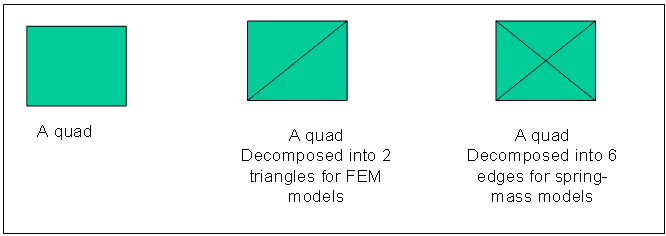
\includegraphics[width=0.95\linewidth]{Quad_Multiple_Topologies}
  \caption{Multiple topology descriptions of the Quad.}
 \label{fig:Quad_Multiple_Topologies}
\end{figure*}

Another important aspect of the design is the fact that topological
changes (mesh cutting or refinement) are handled in SOFA.  For the
programmer, it implies that specific containers must be used to
store data for each software component. For instance, a spring mass
model must store the spring stiffness of each edge. Therefore the
container of spring stiffness must have the same size than the
number of edges in the mesh. In SOFA, to cope with topological
changes that can add or remove the number of edges, it is mandatory
to use a specific container (in such case EdgeData container) that
will automatically resize itself when topological changes occur.

\subsubsection{What are the different mesh topologies supported in SOFA ?}


\subsection{Using Mesh Topologies}

\subsubsection{What is a mesh topology object ?}
\subsubsection{What is the difference with the old MeshTopology object ?}
\subsubsection{What are the different mesh topology objects in SOFA ?}


\begin{figure*}
 \centering
 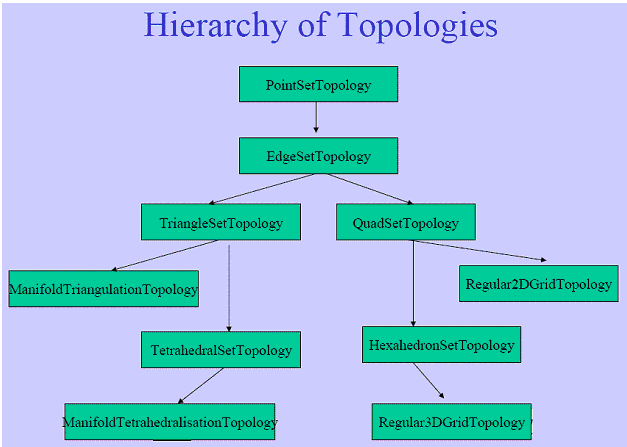
\includegraphics[width=0.95\linewidth]{Hierarchy_Topologies}
  \caption{A generic and hierarchical topology is described from a class called BaseTopology.}
 \label{fig:Hierarchy_Topologies}
\end{figure*}

BaseTopology class provides an implementation which handles
topological changes, full topological relationships and geometric
computation.

\subsubsection{How do I have access to the adjacency information between items ?}
\subsubsection{What to do if I need to know only basic topology information ?}
\subsubsection{What are the geometry algorithms stored in each topology classes ?}

\subsection{Handling Topological Changes}

\subsubsection{How does it work ?}
\subsubsection{What container should I use to handle the topology changes ?}
\subsubsection{How to write the different callback functions associated with the containers ?}

Topological changes are handled in a way which is as much
transparent for the user as possible.


\subsubsection{The 4 components of a BaseTopology object}

\begin{verbatim}

Class BaseTopology<DataTypes> {

// A container for info to be stored and methods to access adjacency :
//   - Adjacency Information is only computed when needed
//   - Non template class
//   - Store TopologicalChange list

TopologyContainer *container ;

// A modifier for low-level methods to change topology :
//   - Cannot be accessed from user
//   - Modifier also changes the DOFs in the Mechanical Object
//   - Low level methods to add or to remove an item
TopologyModifiers<DataTypes> *modifier ;

// TopologyAlgorithms for high-level methods to change topology (user access) :
//   - Accessed from the user
//   - High level algorithms to refine, cut mesh
TopologyAlgorithms<DataTypes> *topologyAlgorithms ;

// Geometry Algorithms methods to get geometry information :
//   - Compute geometric information (normal, curvature, area, length)
GeometryAlgorithms<DataTypes> *geometryAlgorithms ;

};

\end{verbatim}


\subsubsection{Implementation for objects inherited from each other (Point,
Edge, Triangle, Tetrahedron}


\begin{itemize}

 \item PointSetTopology (inherited from BaseTopology) :

    \begin{itemize}

    \item Container : For each point gives its global index. This is useful for subset topologies (subset triangulation, ...) where the number of vertices involved in the topology may not be the same as the total number of vertices.

    \item Modifier : addPointsProcess, removePointsProcess, renumberPointsProcess, addPointsWarning, removePointsWarning, propagateTopologicalChanges

    \item Geometry : computeCenter, computeRadius,
    getAABB()

    \end{itemize}


\item EdgeSetTopology (inherited from PointSetTopology)

    \begin{itemize}

    \item Container : array of edges, array of vertex-edge shell

    \item Modifier : addEdgesProcess, removeEdgesProcess, fuseEdgesProcess, splitEdgesProcess,
   addEdgesWarning, removeEdgesWarning

    \item Geometry : getEdgeLength, getRestEdgeLength

    \end{itemize}


\item TriangleSetTopology (inherited from EdgeSetTopology)

    \begin{itemize}

    \item Container : array of triangles, of vertex- and edge-triangle shell

    \item Modifier : addTrianglesProcess, removeTrianglesProcess, addTrianglesWarning, removeTrianglesWarning

    \item Topology Algorithms : InciseAlongPointsList, RemoveAlongTrianglesList

    \item Geometry : computeTriangleNormal

    \end{itemize}


\item TetrahedronSetTopology (inherited from TriangleSetTopology)

    \begin{itemize}

    \item Container : array of tetrahedra, array of vertex-, edge-, triangle-tetrahedra shell

    \item Modifier : addTetrahedraProcess, removeTetrahedraProcess, addTetrahedraWarning, removeTetrahedraWarning

    \item Geometry : computeTetrahedronVolume

    \end{itemize}

\end{itemize}

\begin{figure*}
 \centering
 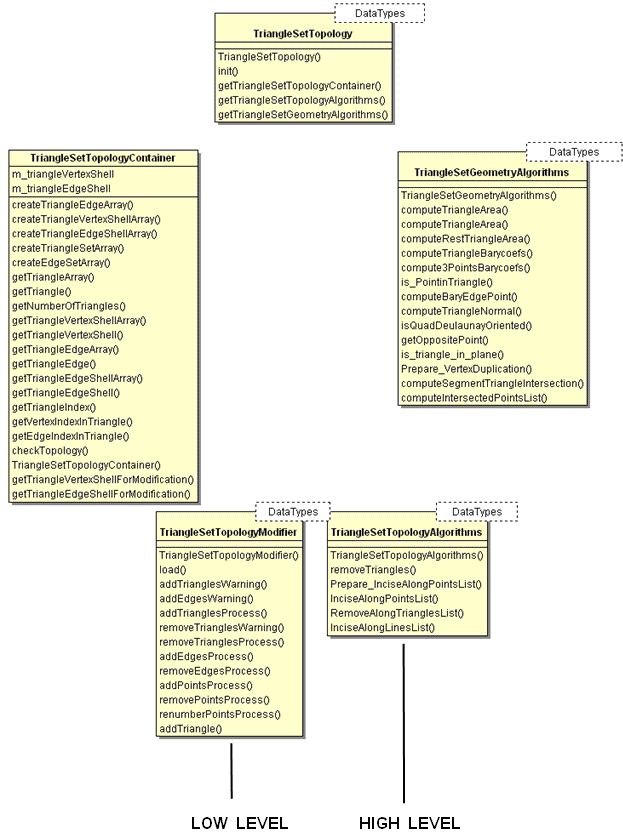
\includegraphics[width=0.95\linewidth]{UML_TriangleSetTopology}
  \caption{UML diagram describing the 4 components of TriangleSetTopology class.}
 \label{fig:UML_TriangleSetTopology}
\end{figure*}

\newpage

\begin{figure*}
 \centering
 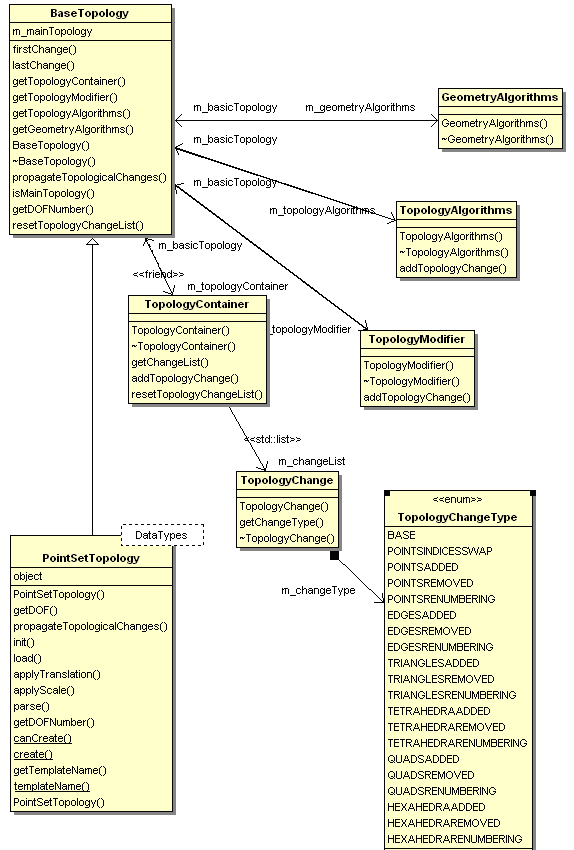
\includegraphics[width=0.95\linewidth]{UML_BaseTopology}
  \caption{UML diagram showing the use of a TopologyChanges List from BaseTopology class.}
 \label{fig:UML_BaseTopology}
\end{figure*}

\newpage

\subsubsection{Definition of data structures to be "aware" of topological
changes}

Force Fields, Constraints, Mapping and other modules may require to
store information for each topological item (point, edge, triangle,
etc.).
\\

Two container data structures are defined to handle topological
changes by matching the types of TopologyChanges :

\begin{itemize}

    \item PointData$<$MyType$>$, EdgeData$<$MyType$>$ are arrays (same as std::vector) of item of type MyType

    \item PointSubset, EdgeSubset are arrays of points or edges

\end{itemize}

Used-defined functions are called when an item is created or
destroyed.
\\

In higher level classes (for example
TriangularQuadraticSpringForceField, DiagonalMass or FixedConstraint
classes), the user only provides callback functions to handle :

\begin{itemize}

    \item the creation of a topological item
    \item the destruction of a topological item

\end{itemize}

\begin{figure*}
 \centering
 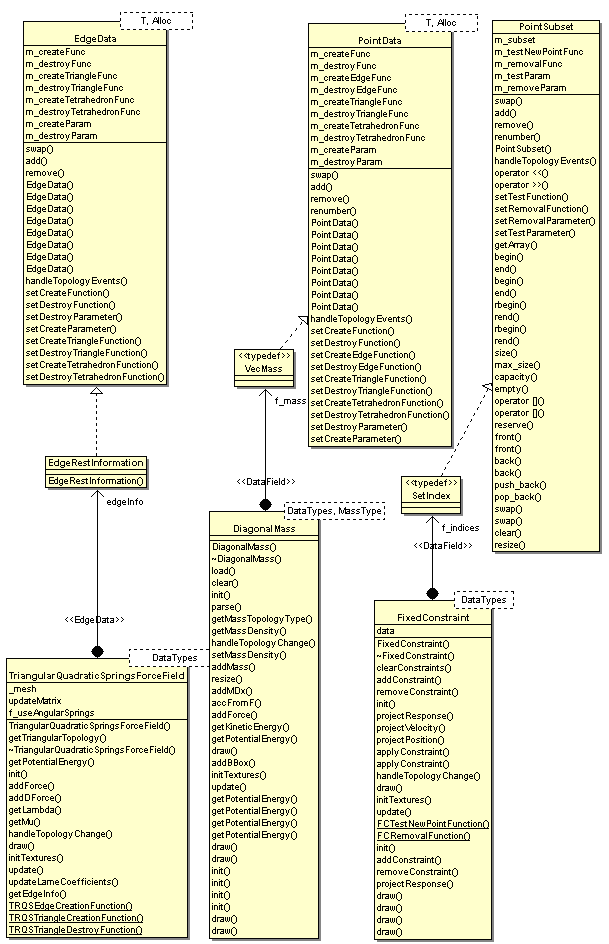
\includegraphics[width=0.95\linewidth, height=0.95\textheight]{UML_Topological_Changes}
  \caption{These UML diagrams show the use of EdgeData, PointData and
PointSubset to handle topological changes implying modifications
respectively in ForceField, Mass and Constraint modules.}
 \label{fig:UML_Topological_Changes}
\end{figure*}

\newpage

\begin{figure*}
 \centering
 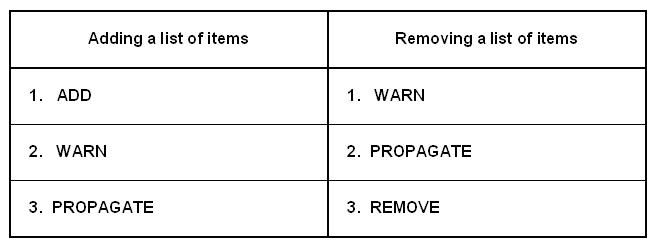
\includegraphics[width=0.95\linewidth]{Order_Notifications}
  \caption{Order to respect when adding or removing an item (see the
explanations in the following example).}
 \label{fig:Order_Notifications}
\end{figure*}

\begin{itemize}

    \item "WARN" means : add the current topological change (add or delete a list of items) in the list of TopologyChanges

    \item "PROPAGATE" means :  traverse the simulation tree with a TopologyChangeVistor to send
    the current topological change event to all force fields, constraints,
    mappings, etc.

\end{itemize}

\subsubsection{Example : What happens when I split an Edge ?}

\begin{figure*}
 \centering
 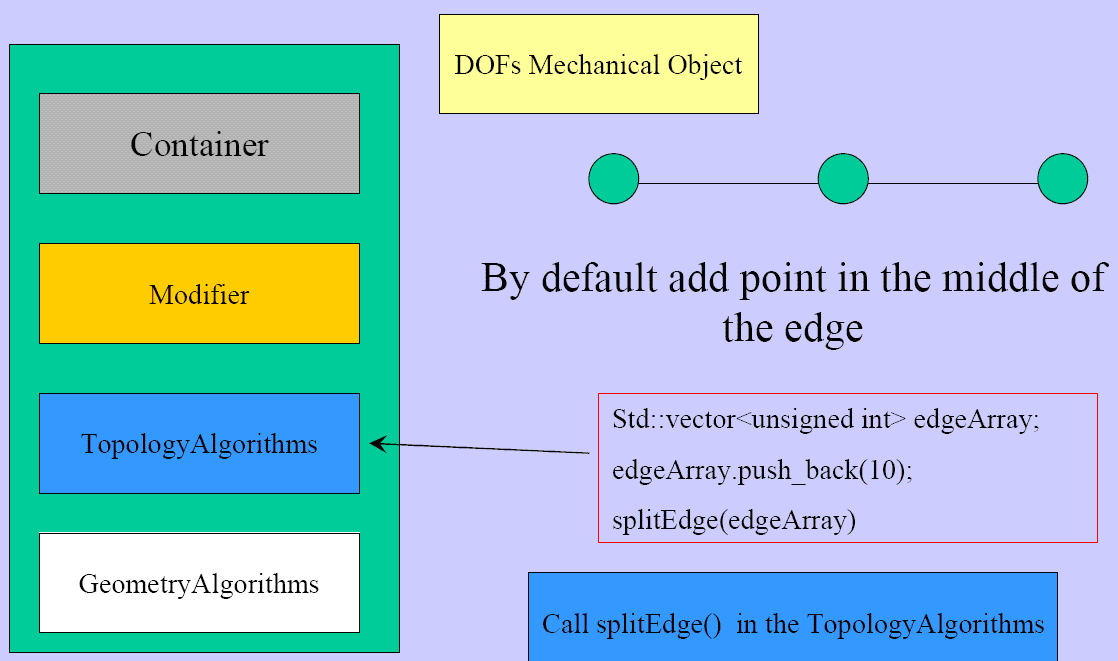
\includegraphics[width=0.95\linewidth]{Topology_Example_1}
 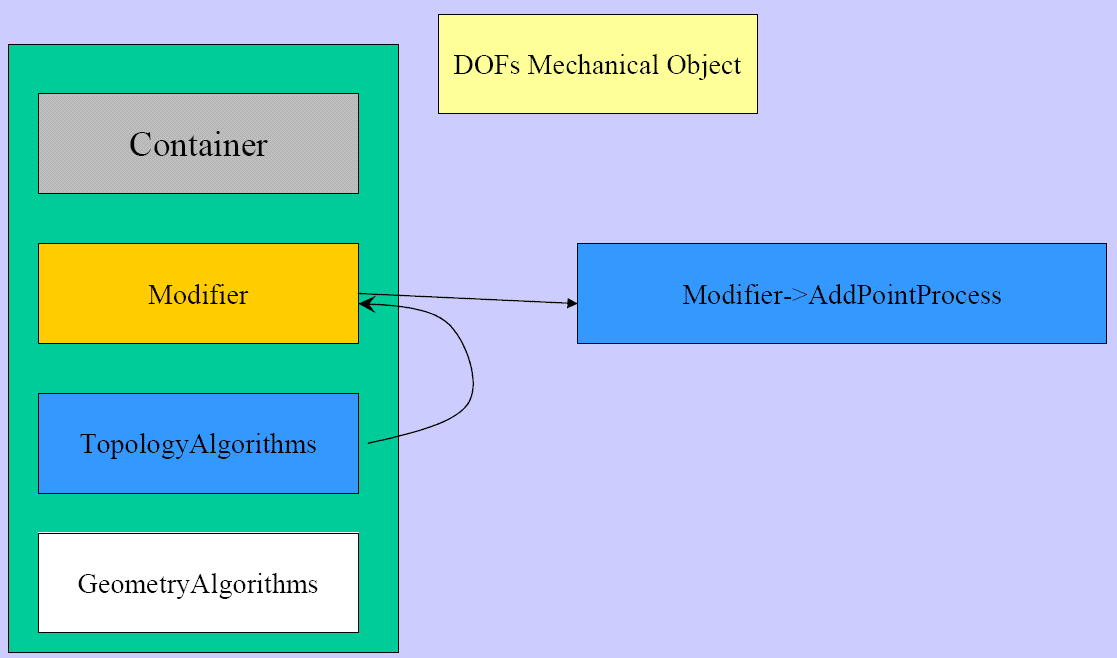
\includegraphics[width=0.95\linewidth]{Topology_Example_2}
  \caption{What happens when I split an Edge ? - Step 1. 2.}
 \label{fig:Topology_Example_12}
\end{figure*}

\newpage

\begin{figure*}
 \centering
 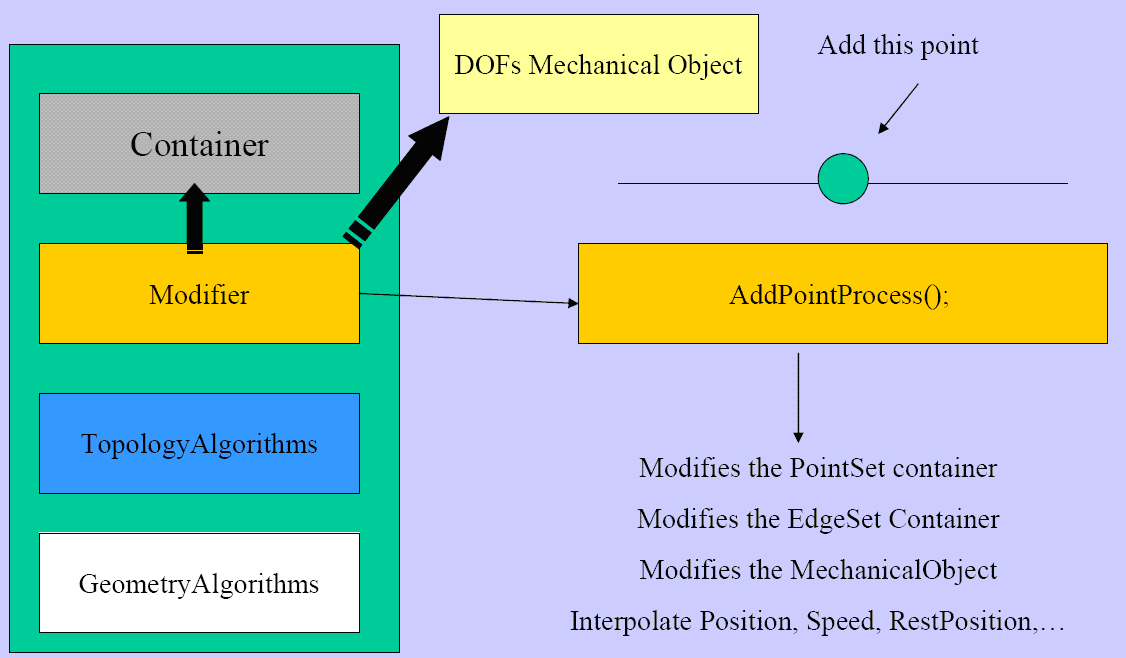
\includegraphics[width=0.95\linewidth]{Topology_Example_3}
 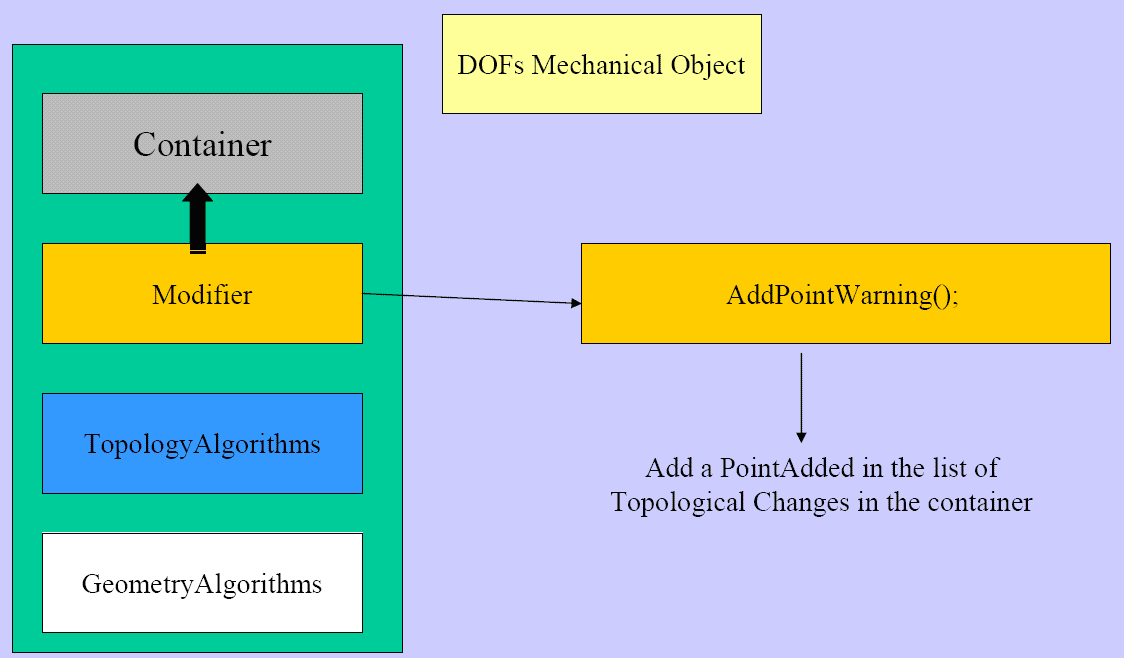
\includegraphics[width=0.95\linewidth]{Topology_Example_4}
  \caption{What happens when I split an Edge ? - Step 3. 4.}
 \label{fig:Topology_Example_34}
\end{figure*}

\newpage

\begin{figure*}
 \centering
 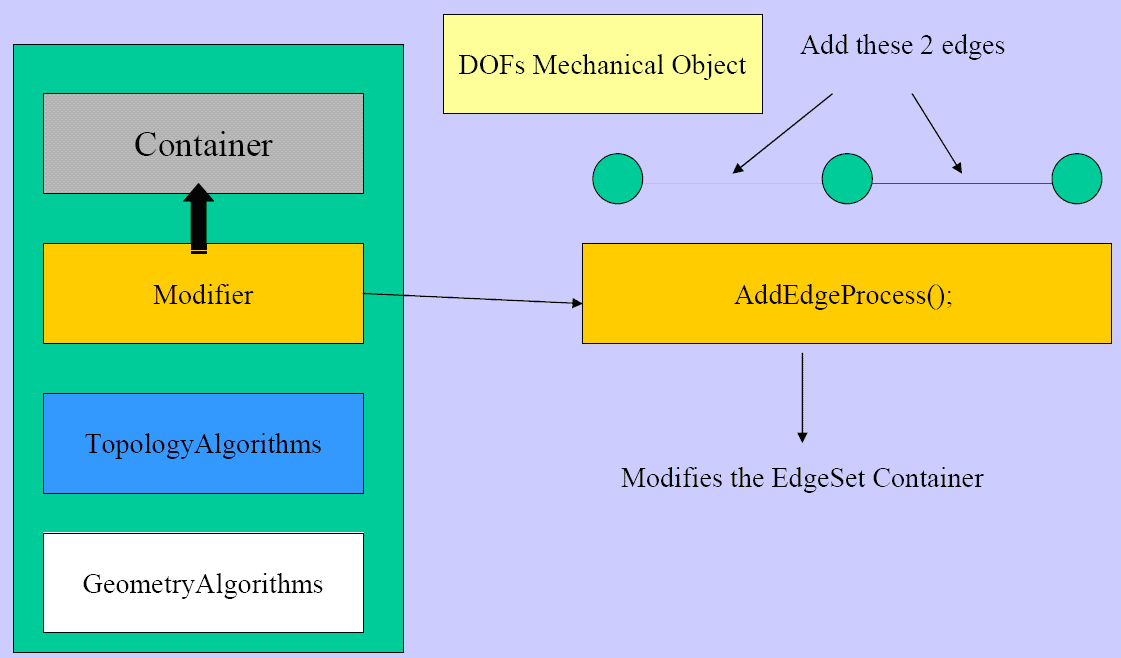
\includegraphics[width=0.95\linewidth]{Topology_Example_5}
 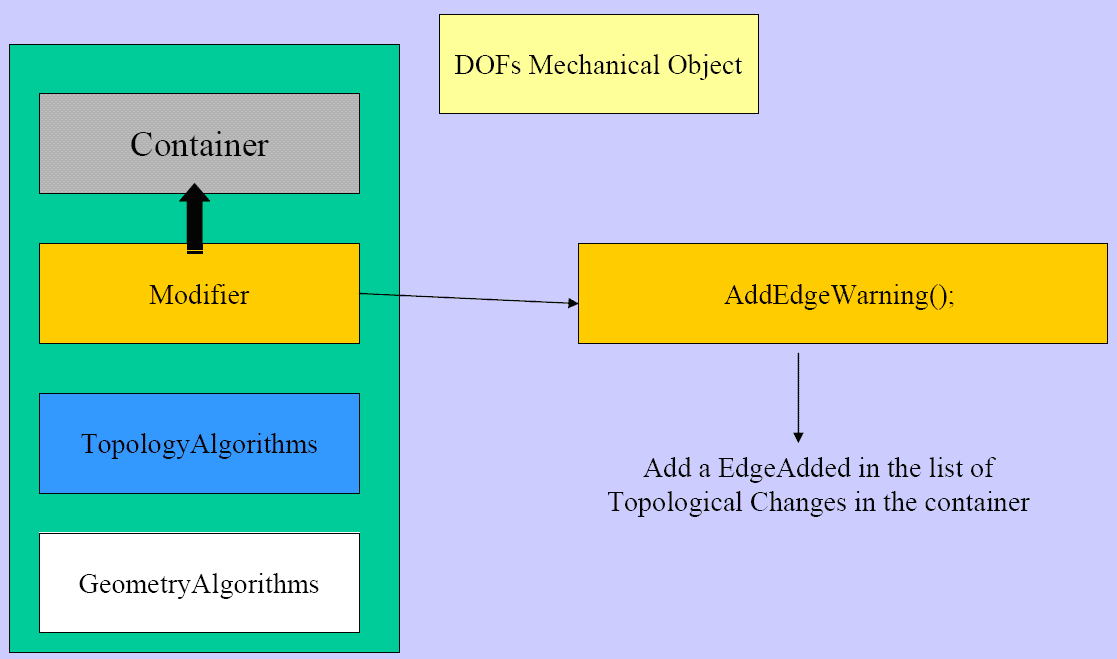
\includegraphics[width=0.95\linewidth]{Topology_Example_6}
  \caption{What happens when I split an Edge ? - Step 5. 6.}
 \label{fig:Topology_Example_56}
\end{figure*}

\newpage

\begin{figure*}
 \centering
 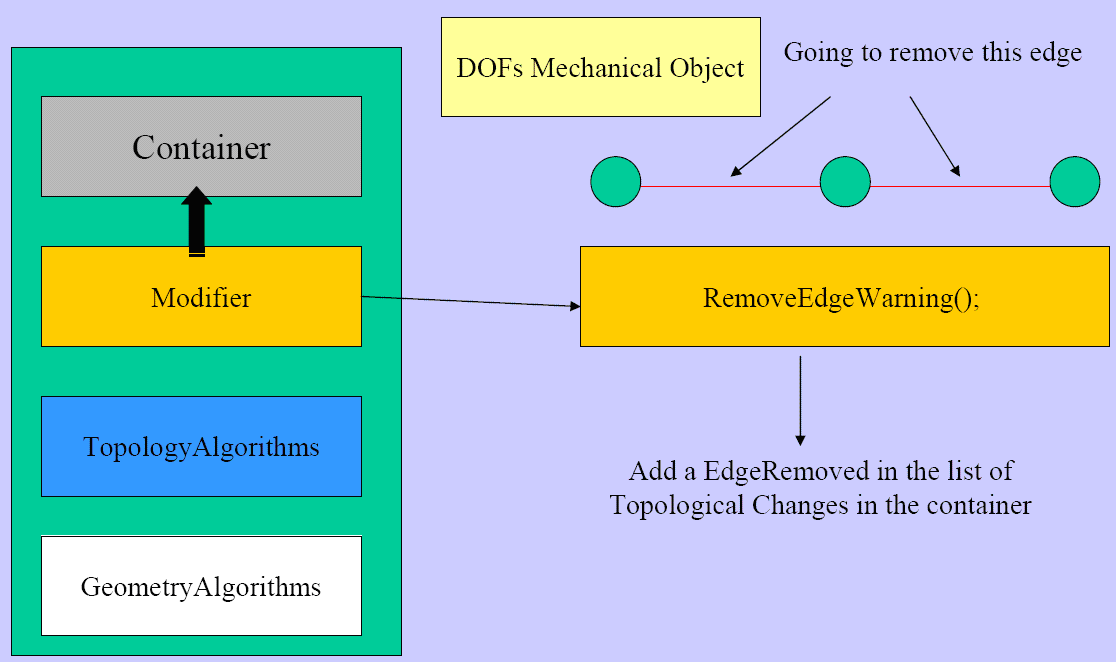
\includegraphics[width=0.95\linewidth]{Topology_Example_7}
 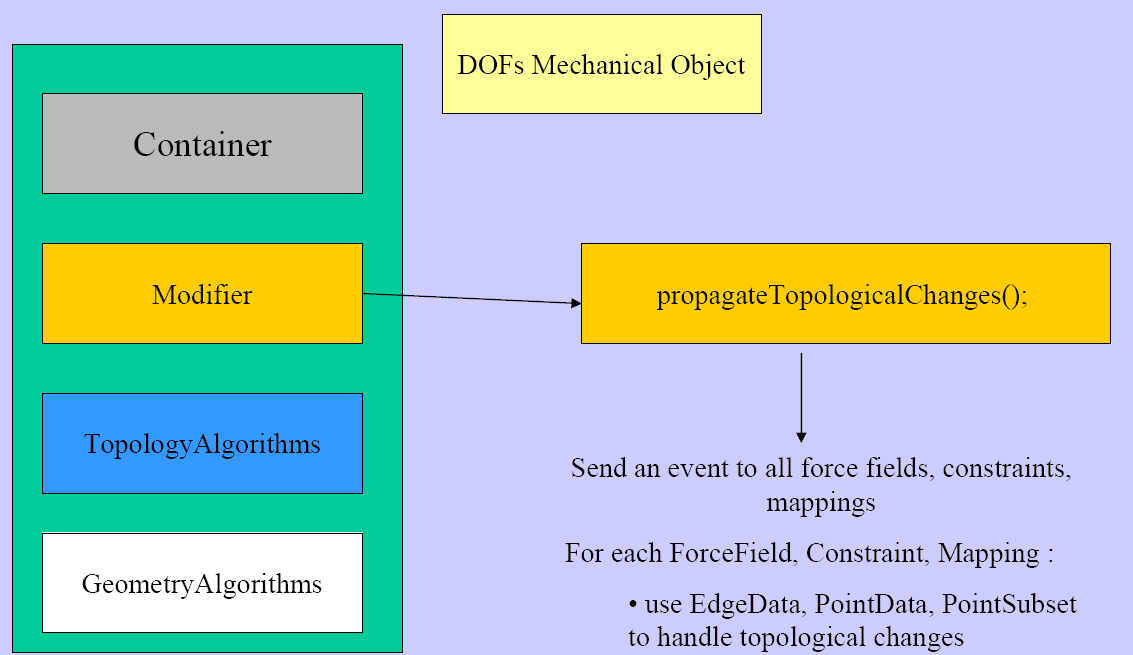
\includegraphics[width=0.95\linewidth]{Topology_Example_8}
  \caption{What happens when I split an Edge ? - Step 7. 8.}
 \label{fig:Topology_Example_78}
\end{figure*}

\newpage

\begin{figure*}
 \centering
 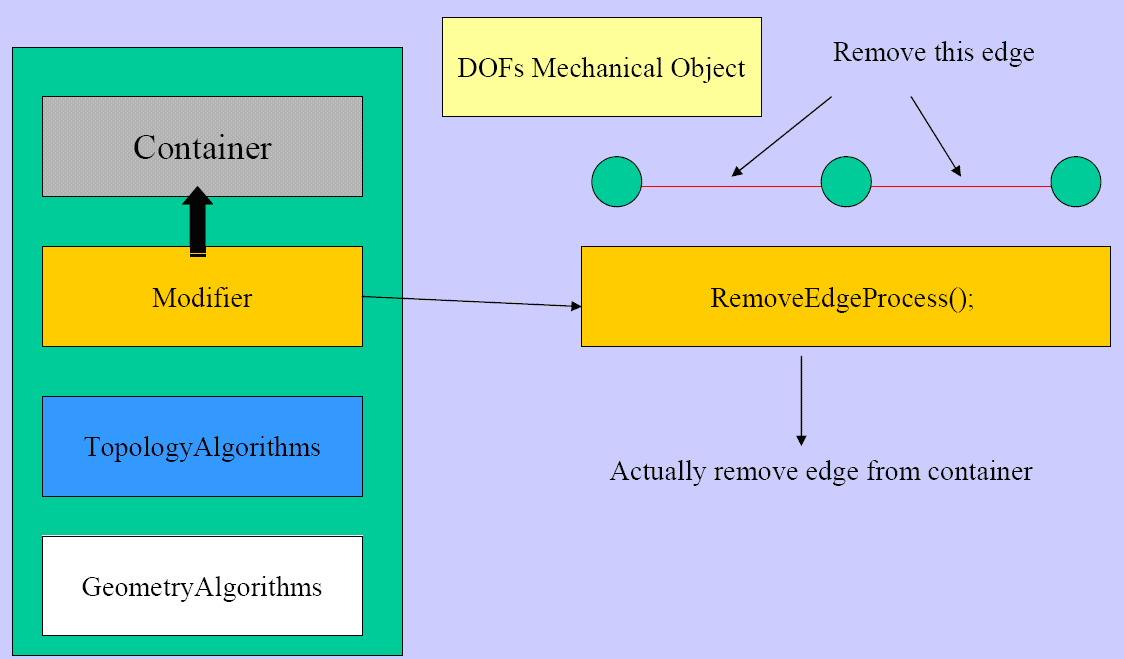
\includegraphics[width=0.95\linewidth]{Topology_Example_9}
  \caption{What happens when I split an Edge ? - Step 9.}
 \label{fig:Topology_Example_9}
\end{figure*}

%%%%%%%%%%%%%%%%%%%% COMPONENTS%%%%%%%%%
%1 STATES
\chapter{States}
\graphicspath{{../states/}}  % to include images
\input{../states/states}


%2 MECA FORCES
\chapter{Mechanical forces}
\emph{to be completed}
\section{ForceField components}

\section{Interaction ForceField}
\label{sec:interactionforcefield}

\section{Mass and inertial forces}

%3 MAPPING
\chapter{Mappings}
\input{../mappings/mappings_body}
\section{Barycentric Mapping}
\section{Rigid Mapping}
\section{Identity Mapping}
\section{Skinning Mapping}


%4 SOLVERS
\chapter{Solvers}
\label{chap:solvers}
\graphicspath{{../solvers/}} 
\section{ODE solvers} 

ODE solvers implement animation algorithms applied at each time step to integrate time and compute positions and velocities one time step forward in time.
% Each step of the algorithm is implemented using a visitor to traverse the scenegraph starting from the node the solver is attached to.
The solvers do not directly address the physical models. 
They apply abstract mechanical operations to state vectors represented by IDs, as illustrated in the algorithm shown in Figure~\ref{fig:eulerexplicit}.
\begin{figure}
\begin{center}
\begin{algorithmic}
\STATE void  \textbf{ExplicitEulerSolver::solve(VecId x, VecId v, double dt)}
\STATE create auxiliary vectors a,f
\STATE resetForce(f)
\STATE accumulateForce(f,x,v)
\STATE computeAcceleration(a,f)
\STATE project(a,a)
\STATE v += a * dt
\STATE x += v * dt
\end{algorithmic}
\caption{Euler's explicit time integration.}
\label{fig:eulerexplicit}
\end{center}
\end{figure}
Each mechanical operation, such as allocating a state vector or accumulating the forces, is implemented using a specialized visitor parameterized on vector IDs or control values such as dt.
This allows to implement the solvers completely independenly of the physical model.
Each vector used by a solver ID is actually scattered over all the state vector containers in the different nodes in the scope of the solver.
Some vector operations such as the dot product apply only to the independent DOFs, stored in the state vectors not attached to a parent by a mapping.
Notice that this design avoids the assembly of global state vectors (i.e. copying Vec3 and quaternions to and from  vectors of scalars).
Moreover, the virtual function calls are resolved at the granularity of the state vectors (i.e. all the particles together, and all the moving frames together) rather than each primitive (i.e. each particle and each frame independently), and allow to optimize each implementation independently.
There is thus virtually no loss of efficiency when mixing arbitrary types in the same simulation.




% The ODE solver creates visitors and applies them to its parent node.
% The ComputeDf visitor presented in Figure~\ref{fig:DfVisitor} finds no mapping nor DOF at the root level (functions are called only if the corresponding component is present in the node), and continues the traversal in the two child branches. 
% Each object computes its own force change df corresponding to its own displacement dx, as previously explained.
% The objects are independent because there is no mapping to a commom DOF component at the scene level.
% Each object manages its own state vectors.
% Thus, using visitors allows the solver to transparently handle an arbitrary number of objects of arbitrary types in the same scene. 
% One can use visitors without knowing to which objects they apply.
% This is a key feature of the SOFA design, which allows us design the algorithms once and to apply them to all types of simulated objects.
% Notice that this design avoids the assembly of global state vectors (i.e. copying Vec3 and quaternions to and from  vectors of scalars).
% Moreover, the virtual function calls are resolved at the granularity of the state vectors (i.e. all the particles together, and all the moving frames together) rather than each primitive (i.e. each particle and each frame independently), and allow to optimize each implementation independently.
% There is thus virtually no loss of efficiency when mixing arbitrary types in the same simulation.
% Hence the ``versatile yet efficient'' motto of SOFA.


We have identified two families of ODE solvers.
The first contains the explicit solvers, which compute the derivative at the beginning of the time step. They are variants of the Euler explicit solver presented in Figure~\ref{fig:eulerexplicit}, and are easily implemented in Sofa using the same operators.
The second family contains the implicit solvers, which consider the derivative at the end or somewhere in the middle of the time step. They typically require the solution of equation systems such as:
\begin{equation}
\label{eq:linear-system}
\underbrace{\left(\alpha \M  + \beta \B  + \gamma \K \right)}_{\mathbf{A}}   \Vdv =  \vec b
%\underbrace{\P \left(\alpha \M  + \beta \B  + \gamma \K \right)}_{\mathbf{A}}   \Vdv =  \vec b
\end{equation}
where $\M$ is the mass matrix, $\K = \frac{\partial \Vf}{\partial \Vx}$ and $\B = \frac{\partial \Vf}{\partial \Vv}$ respectively are the \textit{stiffness} and \textit{damping} matrices (the method is explicit if $\beta$ and $\gamma$ are null). In order to apply simple displacement constraints,  a projection matrix $\P$ can be used, and the system becomes $\P^T \mathbf{A} \P \Vdv =\P^T \vec b $~\cite{baraff98large}.
Implicit integration has the advantage of being more stable for stiff forces or large time steps. However, solving these equation systems requires linear solvers, discussed in the next section.
Currently, eight ODE solvers have been implemented, including symplectic Euler and explicit Runge-Kutta4, implicit Euler and statics solution.



\section{Linear solvers} 
\subsection{Conjugate Gradient} An interesting feature of visitor-based mechanical computations is their ability to efficiently and transparently compute matrix products.
Thus, we have proposed in SOFA an implementation of the Conjugate Gradient, based on the graph traversal. 
The visitor shown in Figure~\ref{fig:DfVisitor} computes the force change \textit{df} based on a given displacement \textit{dx}, as repeatedly performed in Conjugate Gradient algorithm. 
An arbitrary number of forces and projections may be present in all the nodes, resulting in a complicated stiffness matrix, as shown in the following equation:
\begin{equation}
 \label{eq:dfdx}
\vec{df} = \sum_i  \left( \prod_{j \in path(i)} \mat J_j  \right)^T \K_i \left( \prod_{j \in path(i)} \mat J_j  \right) \vec{dx}
\end{equation}
where $\K_i$ is the stiffness matrix of force $i$, matrix $\J$ encodes the first-order mapping relation of a node with respect to its parent, and $path(i)$ is the list of nodes from the solver to the node the force applies to.
\begin{figure}
\begin{center}
\begin{tabular}{c|c}
\begin{minipage}[t]{0.52\linewidth}
\begin{algorithmic}
\STATE bool \textbf{ComputeDfVisitor::topDown}():
\STATE dof.resetF(this.df)
\IF{mapping}
\STATE mapping.applyJ(this.dx)
\ENDIF
% \FORALL {projection P}
% \STATE P.project( this.dx,this.dx )
% \ENDFOR
\RETURN true
\end{algorithmic}
\end{minipage}
&
%  \hspace{0.01\linewidth}
% &
%  \hspace{0.01\linewidth}
% &
 \begin{minipage}[t]{0.46\linewidth}
\begin{algorithmic}
\STATE void \textbf{ComputeDfVisitor::bottomUp}():
\FORALL {forceField F}
\STATE F.addDF( this.df,this.dx )
\ENDFOR
% \FORALL {projection P}
% \STATE P.project( this.df,this.df )
% \ENDFOR
\STATE mapping.applyJT(this.df)
\end{algorithmic}
 \end{minipage}
\end{tabular}
\caption{Computing $df$ given $dx$ using a visitor.}
\label{fig:DfVisitor}
\end{center}
\end{figure}
This complex product is computed using only matrix-vector products and with optimal factoring thanks to the recursive implementation.
It allows us to efficiently apply implicit time integration to arbitrary scenes using the Conjugate Gradient. 
This method allows us to trade-off accuracy for speed by limiting the number of steps of the iterative solution.


\subsection{Direct Solvers} Direct solvers are also available in SOFA. They can be used as preconditionners of the conjugate gradient algorithm~\cite{CADC10} or for directly solving equation \ref{eq:linear-system}.
Their implementation are based on external libraries such as Eigen, MKL and Taucs. 
When dealing with Finite Element Models, the matrices are generally very sparse and 
efficient implementations based on sparse factorizations allow for fast computations. 
Moreover, when dealing with specific topologies, like wire-like structures, tri-diagonal band solvers can be used for extremely fast results in $\mathcal{O}(n)$
These different linear solvers address matrices which  can be stored in different formats, adapted to the numerical library.
%or even not explicitly stored when only matrix-vector products are applied.
The type of matrix is a parameter of the linear solver, and of the visitors the solver uses. 
Ten linear solvers have been implemented in \sofa{}. They can be interchanged to compare their efficiency.

\subsection{From ODE solver to linear solver}

In SOFA, all states of a mechanical object is described by its degree of freedom. The main works for the simulation are filling and inverting a matrix system in order to find the states of mechanical objects by steps of time. This system matrix can be described as below :
 \[
\left[ \textbf{MBK} \right].a=f \text{    ,  or at time n+1 :   }\left[ \textbf{MBK} \right].a_{n+1}=f_{n+1}
\]
where,
\[
\left\{ 
\begin{array}{l}
\textbf{M} \text { : the mass matrix   }  \\
\textbf{B} \text { : the damping matrix   }  \\
\textbf{K} \text { : the stiffness matrix   }  \\
\left[ \textbf{MBK} \right] \text {  : is a linear combination of MBK (not multiplication)   }  \\
a_{n+1} \text { : accelerator field} \\
f_{n+1} \text { : force field} 
\end{array}\right.
\]
 Usually, \textbf{M} is filled by \textbf{mass} components, \textbf{K} is filled by \textbf{forcefield} or \textbf{interactionforcefield} components, \textbf{B} (often $\alpha\textbf{M}+\beta\textbf{K}$ ) and $\left[ \textbf{MBK} \right]$ are computed by \textbf{odesolver} components. The works left to invert the matrix system are done by \textbf{linearsolver} components.
\begin{center}
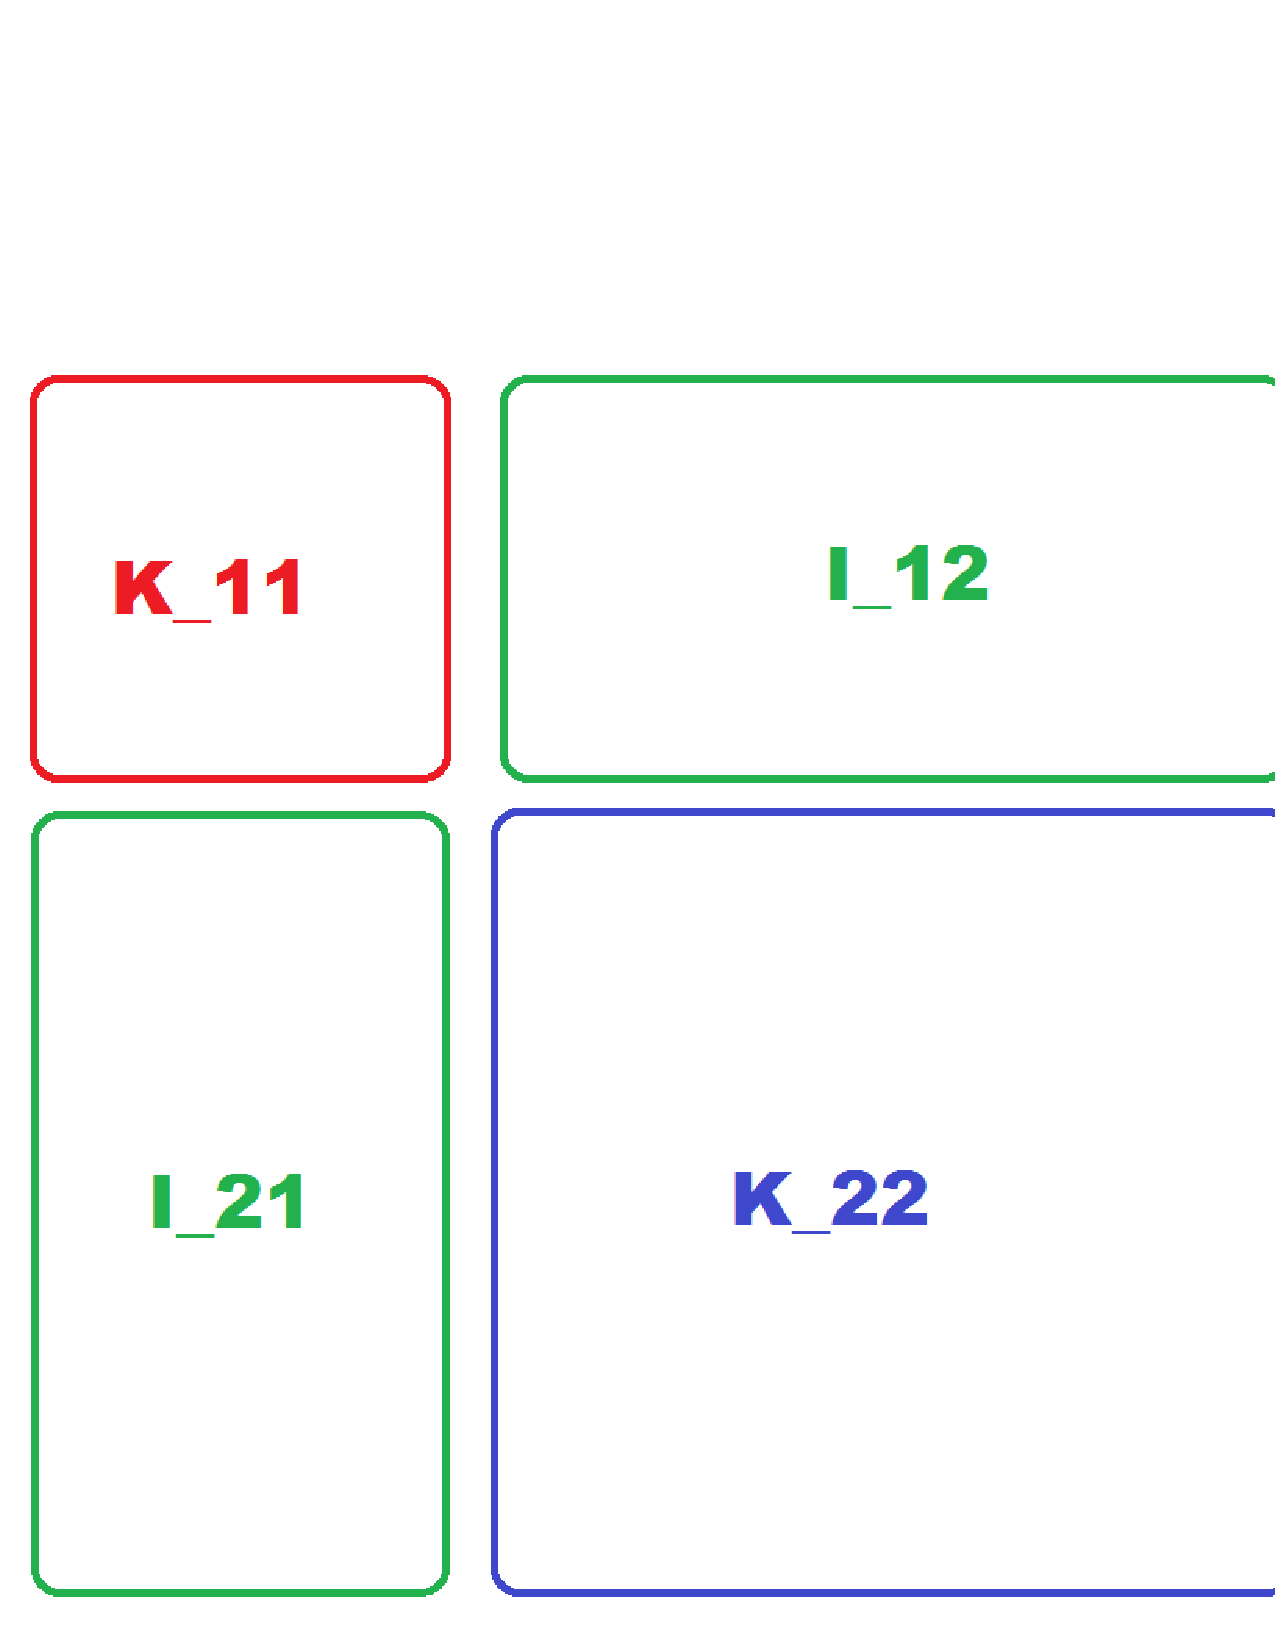
\includegraphics[scale=0.3]{matrix_bloc.pdf}
\end{center}
On the case for example when there are two mechanical objects, we can see a global stiffness matrix describing the two mechanical states, composed diagonal blocs and non-diagonal blocs. The diagonal blocs are filled by \textbf{mass},\textbf{forcefield} components, and the non-diagonal ones are filled by \textbf{interactionforcefield} if existed.
\paragraph{Mapping matrix contribution : } When existe a mapping on the simulation scene, the states of two mechanical objects are relied by : 
\[
\begin{array}{rl}
\textbf{x}_{2} & = \Im\left(\textbf{x}_{1}\right)           \text{      ,	mapping::apply}             \\
\textbf{v}_{2} & = \left[\textbf{J}\right] \textbf{v}_{1}   \text{      ,	mapping::applyJ}  
\end{array}
\]
The $\left[\textbf{J}\right]$ matrix is derivative of $\Im$ operator and is defined by the \textbf{mapping} components. The dynamic and matrix system of the two objects are relied by :   
\[
\begin{array}{rl}
\textbf{f}                  & += \textbf{f}_{1}  +   \left[\textbf{J}\right]^{t} \textbf{f}_{2}         \text{      ,	mapping::applyJT}             \\
\left[ \textbf{MBK} \right] & += \left[ \textbf{MBK} \right]_{1}  + \left[\textbf{J}\right]^{t}  \left[ \textbf{MBK} \right]_{2} \left[\textbf{J}\right]
\end{array}
\]
The resolution of the system with the mapping is done in general :
\[
\left\{ 
\begin{array}{rl}
\textbf{a}^{n+1}        & = \left[ \textbf{MBK} \right]^{-1}  \textbf{f}^{n+1}    \\
\textbf{v}^{n+1}_{1}    & = \textbf{v}^{n}_{1}     + dt.\textbf{a}^{n+1}         \\
\textbf{x}^{n+1}_{1}    & = \textbf{x}^{n}_{1}     + dt.\textbf{v}^{n+1}         \\
\textbf{x}^{n+1}_{2}    &  \text{ ,	mapping::apply }     \\
\textbf{v}^{n+1}_{2}    &  \text{ ,	mapping::applyJ }          
\end{array}
\right.
\]



\subsection{Particular implementation in SOFA}
The direct solver demands to build explicitly the matrix, and invert this matrix after every step of time in order to solve the mechanical response after a solicitation. In SOFA, there are a little more complicated component called mapping, relying geometrical and mechanical properties by master-slave (DOF-mapped object) relation. All changes of geometry or solicitation to one object interfere to other and vice versa. If the mapped object have its own mechanical behavior, it must be counted on the mechanical propagation by the mapping.
\subsubsection{self-stiffness propagation }
\[
\begin{array}{cc}
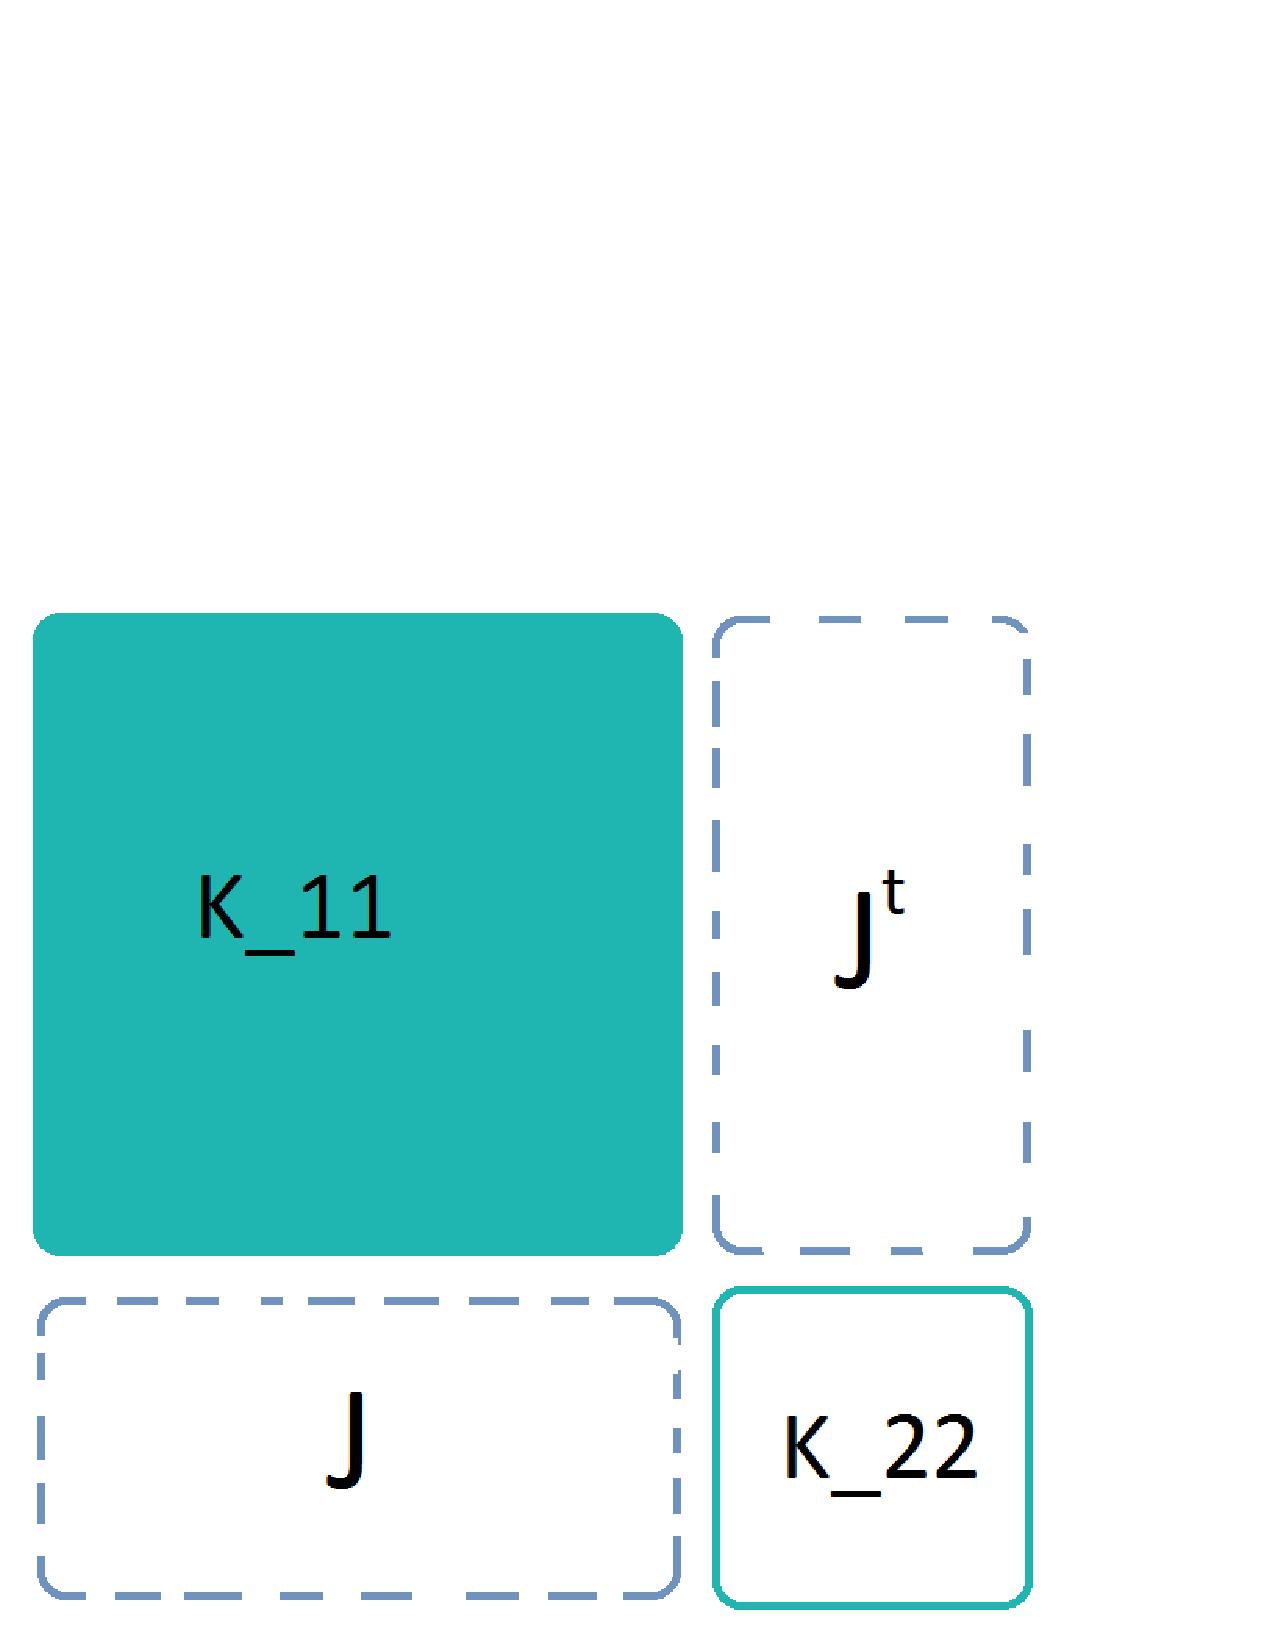
\includegraphics[scale=0.3]{stiffness_propagation_matrix.pdf}        
& 
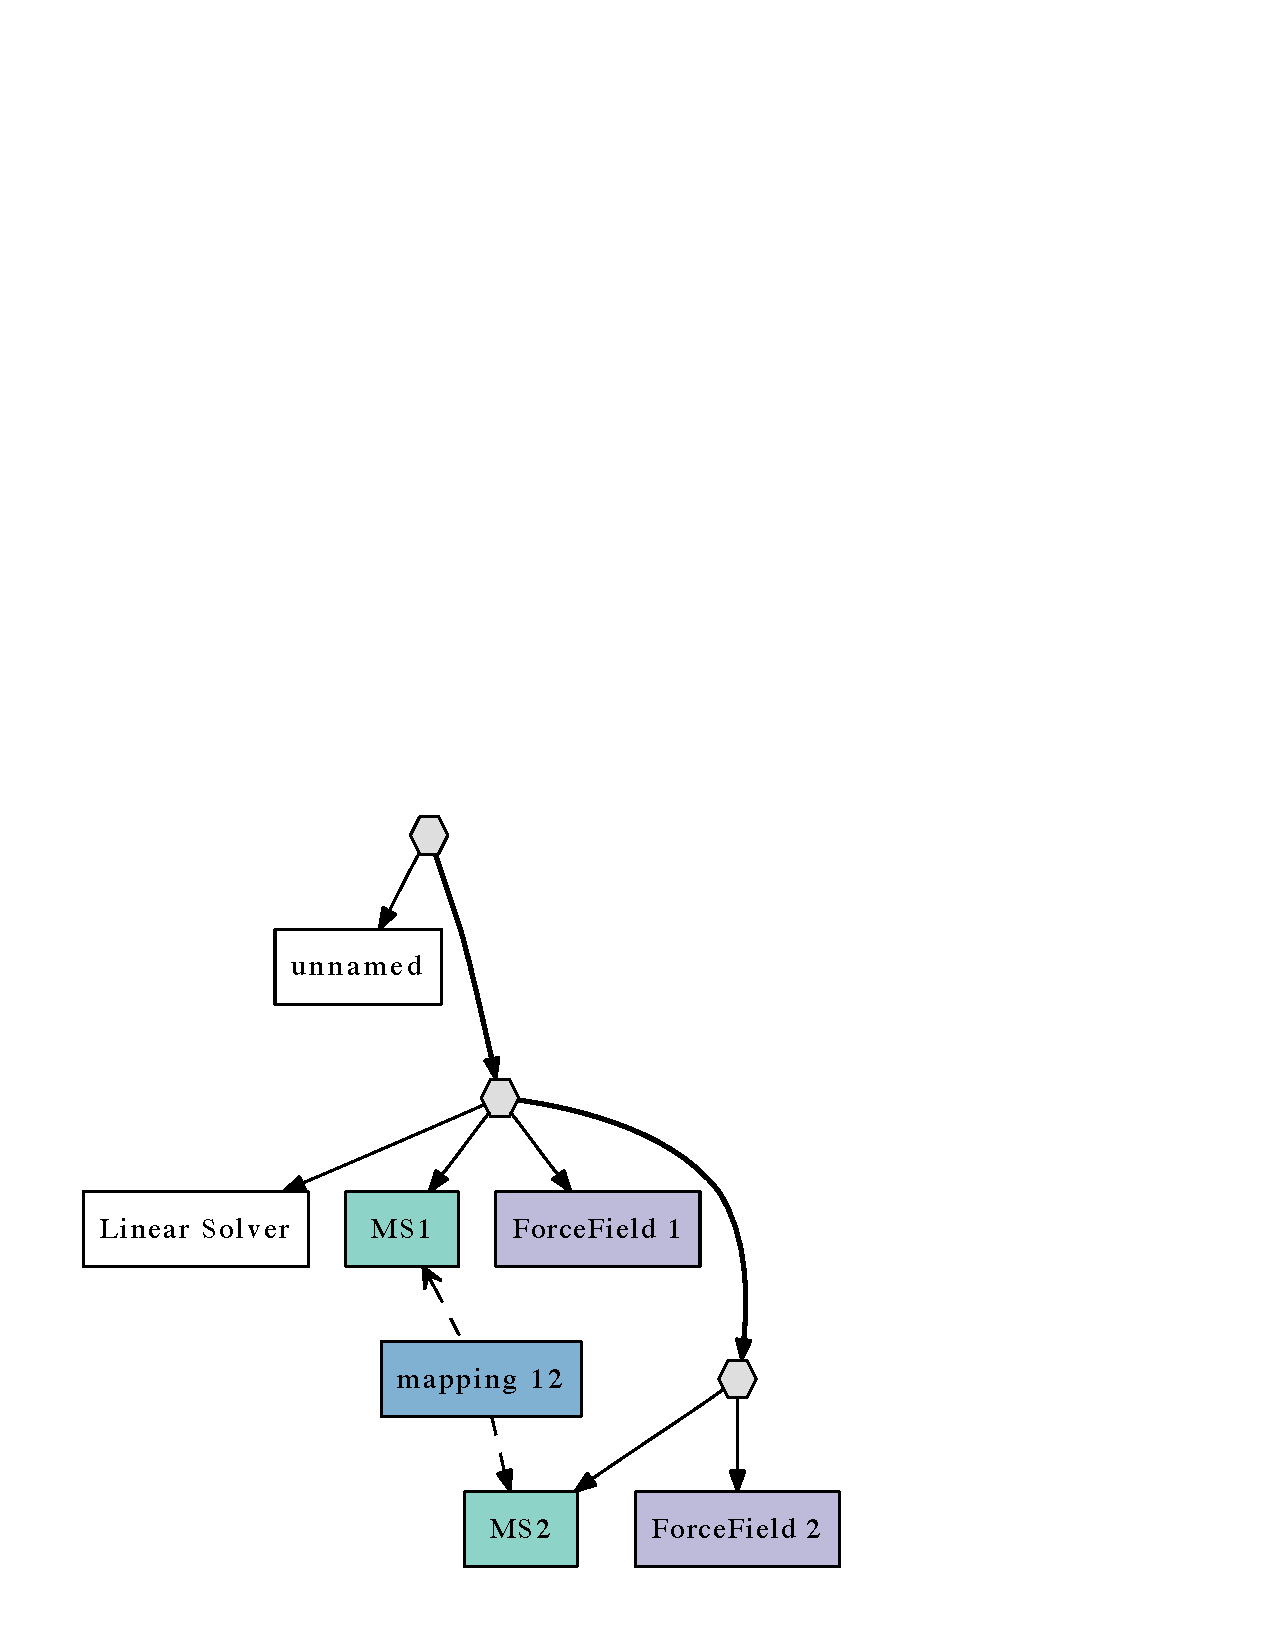
\includegraphics[scale=0.35]{stiffness_propagation.pdf} 
\end{array}
\]
In the simple simulation scene, \textbf{MS2} is a mapped object to the \textbf{MS1} mechanical object by the mapping. The matrix to be inverted for all mechanical response is the filled colorized one ($K_{11}$), the matrix $K_{22}$ describing mechanical properties of the second objects must contribute to $K_{11}$ by the formula :
\[
\left\{ 
\begin{array}{ll}
K_{11}       & += J^t * K_{22} * J               \\
\text{or,}   &         \\
K_{tempo}    & =  J^t * K_{22}                   \\
K_{11}       & += K_{tempo} * J                  \\         
\end{array}
\right.
\]
By doing this computation, we propagate the stiffness of the mapped mechanical object to its root mechanical object.
\subsubsection{interaction-stiffness propagation }
In the general case, the may have a simulation scene where there are many level of mapped mechanical states (mapped of mapped state ...) and many interaction forcefield interacting between them. Therefor the stiffness of interaction forcefield and the mapped mechanical state need to be propagated through the mappings. We can imagine for one propagation, there are two simple cases.
\paragraph{Interaction beweent Real Mechanical Object and Mapped Mechanical Object}
\[
\begin{array}{cc}
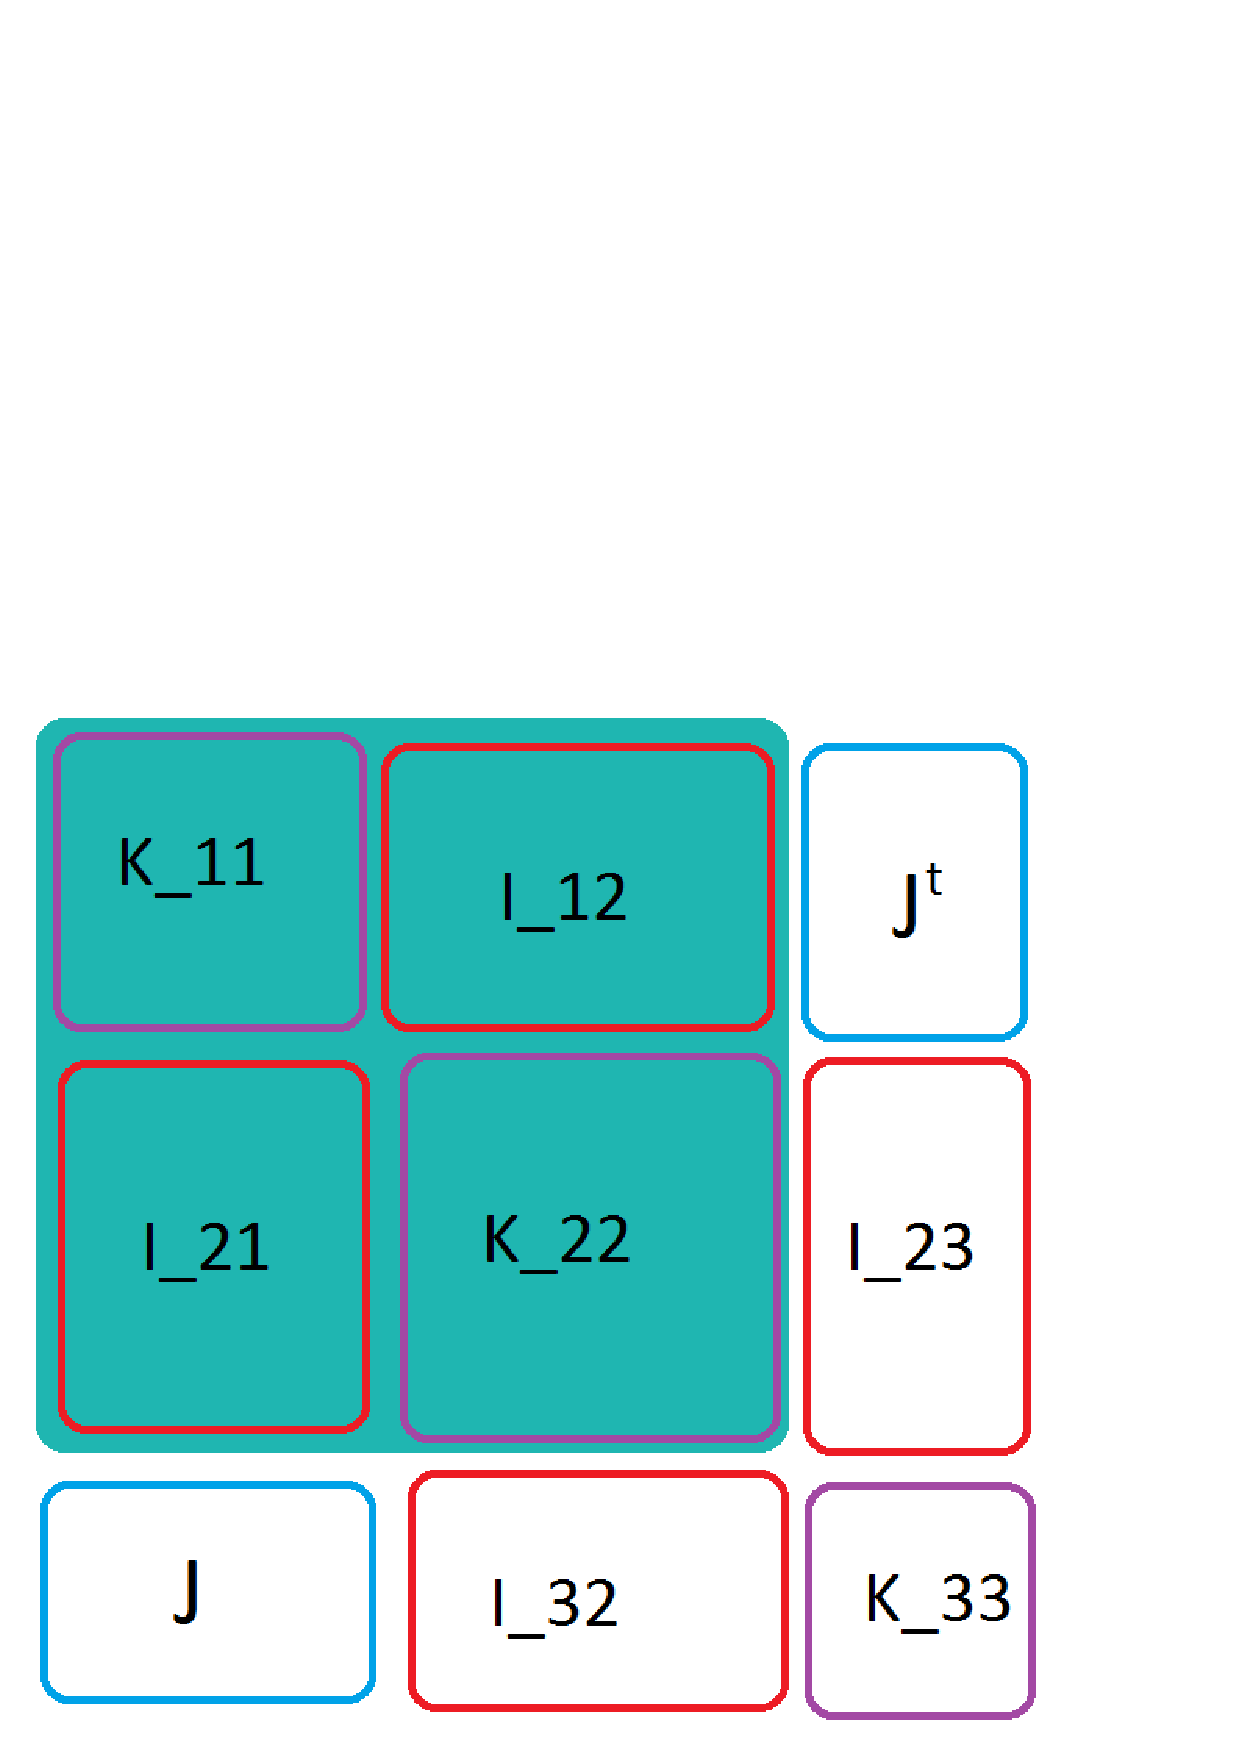
\includegraphics[scale=0.3]{interaction_Real_Mapped_Matrix}        
& 
\includegraphics[scale=0.35]{interaction_Real_Mapped} 
\end{array}
\]
In the case where one of the two mechanical states in interaction is non-mapped, the propagation can be computed directly by the formula :
\[
\left\{ 
\begin{array}{ll}
K_{11}       & += J^t * K_{33} * J               \\
\text{or,}   &                                   \\
K_{tempo}    & =  J^t * K_{33}                   \\
K_{11}       & += K_{tempo} * J                  \\ 
\text{and,}&                 \\      
I_{12}       & += J^t * I_{32}                   \\ 
I_{21}       & += I_{23} * J                        
\end{array}
\right.
\]
\paragraph{Interaction beweent Mapped Mechanical Object and Mapped Mechanical Object}
\begin{center}
  \includegraphics[scale=0.3]{interaction_Mapped_Mapped}
\end{center}
In the case where the two mechanical states in interaction are mapped, the propagation can be computed by two steps. The first consist to propagate the interaction $I_{34}$ to the interation $I_{14}$ :
\[
\left\{ 
\begin{array}{ll}
K_{11}       & += J^t * K_{33} * J               \\
\text{or,}   &                                   \\
K_{tempo}    & =  J^t * K_{33}                   \\
K_{11}       & += K_{tempo} * J                  \\ 
\text{and,}&                 \\      
I_{14}       & += J^t_A * I_{34}                  \\ 
I_{41}       & += I_{43} * J_A                        
\end{array}
\right.
\]
The following step can compute as the one of above paragraph, propagating the interation $I_{14}$ to $I_{12}$.


%In summary, ODE solution is performed using a hierarchy of algorithms and data structures with each level implemented in a different component: the main ODE solution algorithm , the auxiliary linear solver  parameterized by the type of matrix, and an optional preconditioner when the Conjugate Gradient linear solver is used.
%Using a direct solver requires the explicit computation and storage of the system matrix \mat A of Equation~\ref{eq:linear-system}.
%The mass and stiffness matrices are written by the components and summed at each node level. They are then multiplied by the projection and mapping matrices during visitor traversals, and stored in the solver.

\section{Constraint solvers} 
\label{lm}
To handle different kinds of interactions (contact, friction, joints between particles..) between the simulated objects, SOFA allows the use of Lagrange multipliers~\cite{DDKA06}. 
%see \textit{e.g.}\cite{Duriez_eurographics2008}.
%The third family of solvers involves non-trivial constraints requiring additional equations, and additional unknowns called 
They may be combined with explicit or implicit integration.
Each constraint depends on the relative position of the interacting objects, and on optional parameters 
(such as a friction coefficient, etc.)\footnote{For simplicity, we present the equations for two interacting objects 
(rigid or deformable) $1$ and $2$, but the solution applies to arbitrary number of interacting bodies.}:
\begin{equation}
\begin{array}{c}
\Phi(\Vx_1, \Vx_2, ...) = 0 \\ 
\Psi(\Vx_1, \Vx_2, ... ) \geq 0
\end{array}
\label{eq:constraints}
\end{equation} where $\Phi$ represents the bilateral interaction laws (attachments, sliding joints, etc.) whereas $\Psi$ represents unilateral interaction laws (contact, friction, etc.). These functions can be non-linear.
% The solution uses Lagrange multipliers and a single linearization by time step (see~\cite{DDKA06}). 
The Lagrange multipliers are computed at each simulation step.
%However, for interaction including deformations, there is often a temporal coherency on the multipliers values. 
%Thus, we can provide an estimate $\tilde{\lambda}$ at the beginning of each time step and compute a correction $\Delta \lambda$ so that $\lambda = \tilde{\lambda} +\Delta \lambda$.  
They add force terms to Equation (\ref{eq:linear-system}):
\begin{equation}
\begin{array}{c}
\mathbf{A}_1  \Vdv_1 = \mathbf{b}_1 + \mathbf{H}_1^T \lambda\\
\mathbf{A}_2  \Vdv_2 = \mathbf{b}_2 + \mathbf{H}_2^T \lambda
\label{eq:constraint-systeme}
\end{array}
\end{equation}
where 
\begin{equation}
\mathbf{H}_1 = [\frac{\delta \Phi}{\delta \Vx_1} \  ; \  \frac{\delta \Psi}{\delta \Vx_1}  ]\qquad  \mathbf{H}_2 = [\frac{\delta \Phi}{\delta \Vx_2} \  ; \  \frac{\delta \Psi}{\delta \Vx_2}  ].
\end{equation}
Matrices $\mathbf{H}_1$ and $\mathbf{H}_2$ are stored in the mechanical state component of each node. Thus, when the constraint applies to a model that is mapped (see section \ref{sec:mappings}), the constraints are recursively mapped upward like forces to be applied to the independent degrees of freedom~\cite{Duriez_eurographics2008}. 
% An example that illustrates this concept can be found in \cite{Duriez_eurographics2008}. 
Solving the constraints is done by following these steps:


\textbf{Step 1, Free Motion}: interacting objects are solved independently while setting $ \lambda  = 0$. 
We obtain what we call a \textit{free motion} $\Vdv_1^{\mathrm{f}}$  and  $\Vdv_2^{\mathrm{f}}$ for each object. After integration, we obtain $\Vx_{1}^{\mathrm{f}}$ and $\Vx_{2}^{\mathrm{f}}$. 
%For the prediction, use $\tilde{\lambda} = \lambda^{t}$. 
During this step, each object solves equation~(\ref{eq:constraint-systeme}) with $ \lambda  = 0$ independently using a dedicated solver.  

\vspace{2mm}

\textbf{Step 2, Constraint Solving}: 
%the constraint laws are linearized as follows:
%\begin{equation}
%\label{eq:const-lin}
%\underbrace{
%\left[ \! \! \!
%\begin{array}{c}
%\Phi(\Vx_{1}^{t+h}, \Vx_{2}^{t+h})  \\
%\Psi(\Vx_{1}^{t+h}, \Vx_{2}^{t+h}) 
%\end{array} \! \! \!
%\right]}_{\boldsymbol{\delta}^{t+h}}  \! 
%=  \! 
%\underbrace{
%\left[ \! \! \!
%\begin{array}{c}
%\Phi(\Vx_{1}^{\mathrm{f}}, \Vx_{2}^{\mathrm{f}})  \\
%\Psi(\Vx_{1}^{\mathrm{f}}, \Vx_{2}^{\mathrm{f}}) 
%\end{array}\! \! \!
%\right]}_{\boldsymbol{\delta}^{\mathrm{f}}}
% + h\mathbf{H}_1\Vdv_1^{\mathrm{c}}  +  h\mathbf{H}_2\Vdv_2^{\mathrm{c}}
%\end{equation}
%With $\Vdv_1^{\mathrm{c}}$ and $\Vdv_2^{\mathrm{c}}$ being the unknown corrective motion ($\Vdv= \Vdv^{\mathrm{f}} + \Vdv^{\mathrm{c}}$) when solving equation \ref{eq:constraint-systeme} with $\mathbf{b}_1 = \mathbf{b}_2 = 0$. By gathering equations \ref{eq:constraint-systeme} and \ref{eq:const-lin}, we have:
The constrained equations can be linearized and linked to the dynamics (see \cite{CJADLC10} for details). 
\begin{equation}
\left[
\begin{array}{c}
\Phi(\Vx_{1}, \Vx_{2})  \\
\Psi(\Vx_{1}, \Vx_{2}) 
\end{array} \! \! \!
\right]
 =
 % \underbrace{
\left[ \! \! \!
\begin{array}{c}
\Phi(\Vx_{1}^{\mathrm{f}}, \Vx_{2}^{\mathrm{f}})  \\
\Psi(\Vx_{1}^{\mathrm{f}}, \Vx_{2}^{\mathrm{f}}) 
\end{array}\! \! \!
\right]
%}_{ \delta^{\mathrm{f}}  }
 + 
 \underbrace{
 h\mathbf{H}_1\Vdv_1^{\mathrm{c}}  +  h\mathbf{H}_2\Vdv_2^{\mathrm{c}}
 }_{h \left[  \mathbf{H}_1 \mathbf{A}_1^{-1}  \mathbf{H}_1^T + \mathbf{H}_2 \mathbf{A}_2^{-1}  \mathbf{H}_2^T \right]\lambda
 }
 %=
 %\delta^{\mathrm{f}} +
%\underbrace{h \left[  \mathbf{H}_1 \mathbf{A}_1^{-1}  \mathbf{H}_1^T + \mathbf{H}_2 \mathbf{A}_2^{-1}  \mathbf{H}_2^T \right]}_{\mathbf{W}} \lambda
\label{eq:addjminvjt}
\end{equation}
With $\Vdv^{\mathrm{c}} = \Vdv - \Vdv^{\mathrm{f}}$. 
Together with equation (\ref{eq:constraints}), these equations compose a Mixed Complementarity Problem that can be solved by a variety of solvers.
We compute the value of $ \lambda$ using a projected Gauss-Seidel algorithm that iteratively checks and projects the various constraint laws contained in $\Phi$ and  $\Psi$ ~\cite{DGMCG09}. 

\textbf{Step 3, Corrective Motion}: when the value of $\lambda$ is available, the corrective motion is computed as follows:
%
\begin{equation}
\label{eq:corrective-motion}
\begin{array}{c}
\Vx_{1}^{t+h} =  \Vx_{1}^{\mathrm{f}} + h \Vdv_1^{\mathrm{c}} \  \  \mathrm{ with } \  \  \Vdv_1^{\mathrm{c}} = \mathbf{A}_1^{-1}  \mathbf{H}_1^T \lambda \\
\Vx_{2}^{t+h} =  \Vx_{2}^{\mathrm{f}} + h \Vdv_2^{\mathrm{c}} \  \  \mathrm{ with } \  \  \Vdv_2^{\mathrm{c}} = \mathbf{A}_2^{-1}  \mathbf{H}_2^T \lambda
\end{array}
\end{equation}
%

A Master Solver, which is generally placed at the top of the graph of SOFA has the role of imposing this new scheduling to the rest of the graph. 
%
\begin{figure}[!htb]
\centering
% FreeMotionScheme is missing from SVN
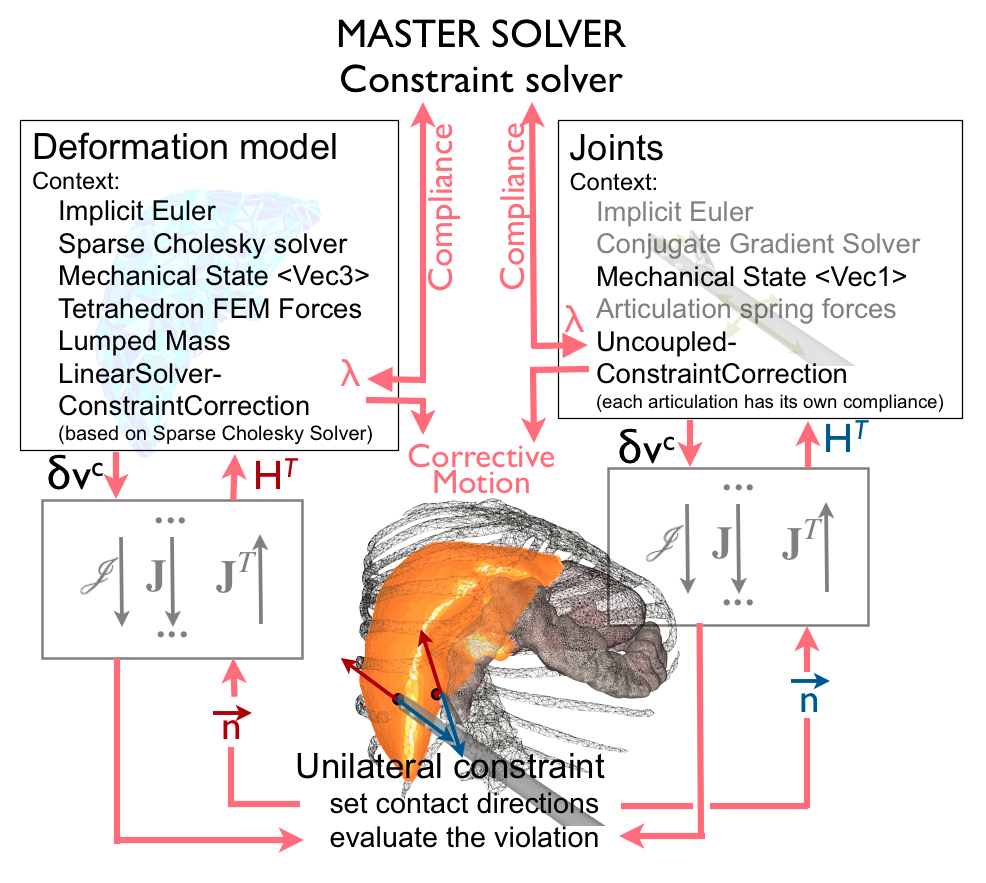
\includegraphics[width= 0.9\columnwidth]{ConstraintSolver.png}
\caption{Contact process using constraints: A unilateral constraint is placed at the level of the contact points. The constraint direction is mapped to the degrees of freedom of the objects to obtain matrix $ \mathbf{H}^T$. The \textit{ConstraintCorrections} components compute the compliance to obtain equation \ref{eq:addjminvjt}. The Constraint solver found a new value of $\lambda$ which is sent to the  \textit{ConstraintCorrections} to compute an adequate corrective motion. The Master Solver is placed at the root of the simulation graph to impose the steps of the simulation process.  }
\label{shema_ToH}
\end{figure}

\textbf{Compliance computation} : Equations~\ref{eq:addjminvjt} and~\ref{eq:corrective-motion} involve the inverse of matrix $\mathbf{A}$ (called compliance matrix), which changes at every time step namely in case of a non-linear model. 
Depending on the simulation case, computing this inverse could be time consuming for real-time simulation. 
When this is too time-consuming, we propose several strategies to improve the speed of the algorithm such as using the diagonal of $\mathbf{A}$ instead of the hole matrix, or a precomputed inverse~\cite{Saupin08}, or an asynchronous factorization on the GPU~\cite{CourtecuisseMICCAI11}.  
These strategies are implemented in a category of components, called  \textit{ConstraintCorrections} that provide different ways of computing $\Vdv^{\mathrm{c}}$ given a value of $\lambda$. Given a simulation, it is very easy to make tests and chose the better solution.








%5 COLLISION
\chapter{Collision detection}
\graphicspath{{../collision/}} 
Collision detection is split in several phases, each implemented in a different component, and organized using a collision pipeline component.
Each potentially colliding object is associated with a collision geometry based on or mapped from the independent DOFs.
The broad phase component returns pairs of colliding bounding boxes (currently, axis-aligned bounding boxes).
Based on this, the narrow phase component returns pairs of geometric primitives with the corresponding collision points.
%\ff{Several collision detection approaches have been implemented: distances between pairs of geometric primitives (triangles and spheres), points in distance fields, distances between colliding meshes using ray-tracing~\cite{HerFauRaf08}, and intersection volume using images as sketched in Section~\ref{sec:LDI}.}
This is passed to the contact manager, which creates contact interactions of various types based on customizable rules.
Repulsion has been implemented based on penalties or on constraints using Lagrange multipliers, and is processed by the solvers together with the other forces at the next time step.
%If topological changes such as cutting operations are triggered, they are handled by the topology algorithms discussed in Section~\ref{sec:topologicalChanges}.
This framework has allowed us to efficiently implement popular proximity-based repulsion methods as well as novel approaches based on ray-casting~\cite{HerFauRaf08} or surface rasterization~\cite{FauBarAllFal08,AFCFDK10}.
Its main limitation is that the contacts can be mechanically processed only after they all have modeled by the collision pipeline.
This does not allow to mechanically react to a collision as soon as it is detected, possibly avoiding further collisions between primitives of the same objects.

When stiff contact penalties or contact constraints are created by the contact manager, an additional \textit{GroupManager} component is used to create interaction groups handled by a common solver, as discussed in Section~\ref{sec:scenes}. 
When contacts disappear, interaction groups can be split to keep them as small as possible.
The scenegraph structure thus changes along with the interaction groups.


\vspace{1cm}
\emph{to be completed}


%6 VISUAL
\chapter{Visual Rendering}


%7 HAPTIC
\chapter{Haptic Rendering}
\label{chap:haptic}
\graphicspath{{../haptic/}} 
The main interest of interactive simulation is that the user can modify the course of the computations in real-time.
This is essential for surgical simulation : during a training procedure, when a virtual medical instrument comes into contact with some models of a soft-tissue, \emph{instantaneous} deformations must be computed.
This visual feedback of the contact can be enhanced by haptic rendering so that the surgeon can really "feel" the contact.

There are two main issues for a platform like SOFA for providing haptic: The first is that haptic forces need to be computed at $1kHz$ whereas real-time visual feedback (without haptic) is obtained at $30Hz$. The second is that haptic feedback can add artificially some energy inside the simulation and can create instabilities, if the control is not \emph{passive}. 

Thus two different approaches are currently implemented into SOFA. The first one is the \emph{Virtual Coupling} technique and the other, more advanced, allows for rendering the constraints presented in section \ref{lm}.



\section{Virtual Coupling} Plugging of a haptic device is bidirectional: the user applies some motions or some forces on the device and this device, in return, applies forces and/or motions to the user.
The majority of the haptic devices propose a \emph{Impedance} coupling: the position of the device is provided by the API and this API asks for force values from the application.
A very simple scheme of coupling, presented in Fig\ref{fig:haptic1}, could have been used.
In this \emph{Direct coupling} case, the simulation would play the role of a controller in an open loop. 

\begin{figure}
\centering
 
\includegraphics[width=0.7\linewidth]{haptic1.png}
 \caption{Direct coupling}
 \label{fig:haptic1}
\end{figure}

Such design is not suitable when stable and robust haptic feedback on a virtual environment is desired. Indeed some combination of the environment impedance and human user reactions can destabilize the system \cite{Adams99}. 
To avoid this, a virtual mechanical coupling is set. It corresponds to the use of a damped-stiffness between the position measured on the device and the simulated position in the virtual environment (see Fig\ref{fig:haptic2}). If very stiff constraints are being simulated then, the stiffness perceived by the user will not be infinite but will correspond to the stiffness of this virtual coupling. 
Hence, a compromise between stability and performance must be found by tuning the stiffness value of the coupling.

\begin{figure}
\centering
 
\includegraphics[width=\linewidth]{haptic2.png}
 \caption{Virtual coupling technique. A 6 DoFs Damped spring is placed between the haptic loop and the simulation.}
 \label{fig:haptic2}
\end{figure}

The damped spring is simulated two times. One time in the haptic loop and one time in the simulation loop. 
If the two loops are synchronized, then the result is the same. But it can also be used in asynchronous mode: fast update of the haptic loop and low rates in the simulation.
In such case, the haptic feedback remains stable but the delay between the two loop is creating an artificial damping.
There is an option to cancel this artificial damping if no contact is detected in the simulation. However, this option can create a sensation of sticking contacts. 
The main advantage of the virtual coupling technique is that it can be easily employed with every simulation of SOFA. The main drawback is that the haptic rendering is not transparent.
 
\section{Constraint-based rendering} An innovative way of dealing with haptic rendering for medical simulation has been proposed in the context of SOFA (see\footnote{The implementation of  \cite{Saupin08} is available in open-source, for the implementation of \cite{Peterlik11}, please contact: christian.duriez@inria.fr }  \cite{Saupin08} and \cite{Peterlik11}). 
The approach deals with the mechanical interactions using appropriate force and/or motion transmission models named \emph{compliant mechanisms} (see Fig\ref{fig:haptic3}). 
These mechanisms are formulated as a constraint-based problem (like presented in section \ref{lm}) that is solved in two separate threads running at different frequencies. 
The first thread processes the whole simulation including the soft-tissue deformations, whereas the second one only deals with computer haptics. 
With this approach, it is possible to describe the specific behavior of various medical devices while relying on a unified method for solving the mechanical interactions between deformable objects and haptic rendering.  
\begin{figure}
\centering
 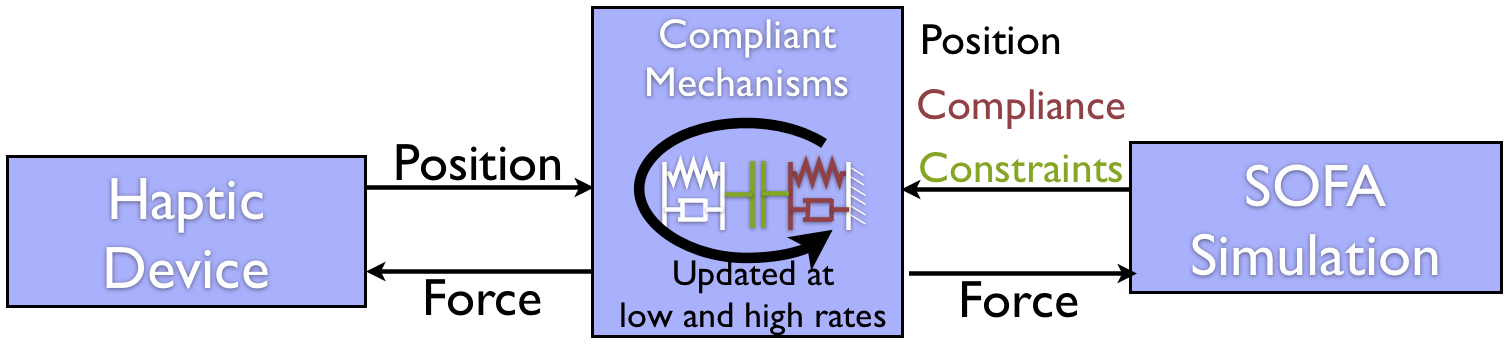
\includegraphics[width=\linewidth]{haptic3.png}
 \caption{Compliant mechanisms technique. The simulation shares the mechanical compliance of the objects and the constraints between them. The constraint response is being computed at low rate within the simulation and at high rates within a separate haptic thread. A 6 DoFs Damped spring is still used to coupled the position of the device to its position in the simulation}
 \label{fig:haptic3}
\end{figure}

\section{How to use it in SOFA ?}
Please see the web page: http://wiki.sofa-framework.org/wiki/Haptic  and use the tutorial "dentistry".



\pagebreak
\part{Design and Development}
\pagebreak

%%%%%%%%%%%%%%% OLD CHAPTERS %%%%%%%%%%%
% This chapter is borrowed from a stand-alone document defined in directory design/
\chapter{Design}
\graphicspath{{../design/}}  % to include images
\begin{wrapfigure}{r}{0.5\textwidth}%
\centering%
\vspace{-1cm}
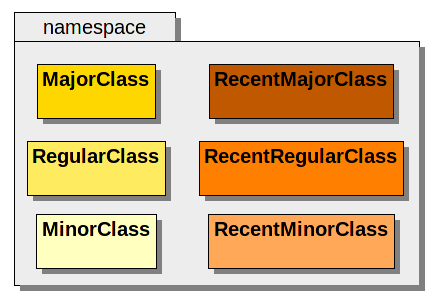
\includegraphics[scale=.33]{../classdiagrams/uml-legend.png}%
\caption{Color conventions in UML diagrams.}%
\label{fig:uml-legend}%
\end{wrapfigure}%

\section{Introduction}

This chapter present the design of \sofa{}, as well as its recent evolutions.
It also includes discussions justifying some of the decision that are behind this design.

The conventions used in UML class diagrams are presented in Fig~\ref{fig:uml-legend}.

\vspace{.8cm}

\section{Core Class Diagrams}

\subsection{Object Model (\textcode{sofa::core::objectmodel})}

\begin{figure}[h]
\centering
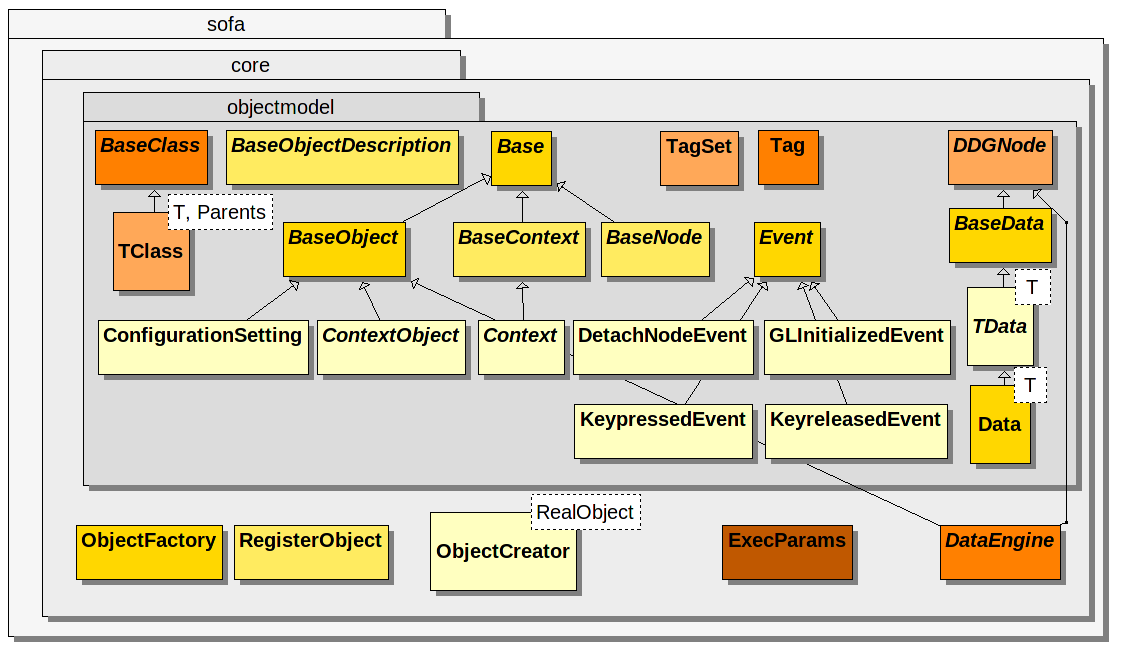
\includegraphics[scale=.33]{../classdiagrams/sofacore-objectmodel.png}
\caption{Classes of the \textcode{sofa::core::objectmodel} namespace.}
\label{fig:uml-sofa-core-objectmodel}
\end{figure}

\subsubsection{Changes compared to the 1.0~beta~4 version}\label{sec:design-core-objectmodel-changes}

\paragraph{New class description system.}
It is based on the \textcode{BaseClass} and \textcode{TClass} classes, and requires to add the \textcode{SOFA\_CLASS} macro in the declaration of all classes deriving from Base.
The benefits are that it is now possible to follow the full hierarchy of classes from the final components, instead of having just a fixed set of categories.
This macro is also necessary in classes with a templated parent class to be able to use methods and member variables defined in \textcode{Base} such as \textcode{initData} or \textcode{sout}. This removed all the previously redundant direct heritage to \textcode{BaseObject} that was previously required.

\paragraph{Objects and node tagging (\textcode{Tag} and \textcode{TagSet}).}
The goal of the introduction of tags is to provide one of the pieces necessary to support non-mechanical states (electrical potentials, constrast agent concentrations) as well as cleaner non-geometrical mechanical states (fluid dynamics, reduced-coordinate articulations).
For example, in a simulation involving blood in deformable vessels, we would use two tags to distinguish the different states : mechanical, fluid.
These tags will be used to easily work with only a subset of the components, so that the mechanical solver works on positions and forcefields but don't interferes with blood flow and pressure, and inversely for the fluid solver\footnote{\url{http://wiki.sofa-framework.org/tdev/wiki/Notes/ProposalGenericStates}}.
We decided on using there tags instead of extending the class hierarchy as was done before with the \textcode{State} and \textcode{MechanicalState} classes.
A hierarchy is fine when we have only one feature that we want to differentiate on (such as base vs mechanical vs electrical), but when we add other criteria (lagrangian geometry vs eulerian vs reduced generalized coordinates, velocity vs vorticity, independent vs mapped DOFs) it is no longer manageable as specialized classes.
A secondary use of these tags is to replace existing subsets mechanisms within CollisionModels (r2441) and Constraints (r3121).
The design is based on the following elements.
Tags are added to BaseObject, as a list of string (internally converted to a list of unique ids for faster processing).
All visitors now filter the objects they process based on their list of tags.
All solvers by default copy their own list of tags to the visitors they execute, so that they only affect the objects with the same tags as they have (TODO: this is currently broken). 

\paragraph{Dependencies between Data (\textcode{DDGNode} and \textcode{DataEngine}).}
The goal is to be able to specify simple links between datas or through computation engines.
To function correctly, the methods \textcode{getValue()} or \textcode{beginEdit()}/\textcode{endEdit()} are required to be called in all codes accessing values contained in Data instances.
To enforce this, the class DataPtr was removed.
Note also that it is very inefficient to call \textcode{getValue()} repetively within computation loops.
Instead, the recommanded method is to use the helper classes \textcode{ReadAccessor} and \textcode{WriteAccessor}
that can hold a reference to a \textcode{Data} value, provides the same API as regular vectors,
and automatically calls \textcode{endEdit()} at the end of the call block in case of \textcode{WriteAccessor}.

\textbf{TODO:} \textit{\textcode{TData<T>} was useful as a common parent for \textcode{Data<T>} and \textcode{DataPtr<T>}, but now that \textcode{DataPtr} no longer exist, it would simplify the hierarchy to merge \textcode{TData<T>} and \textcode{Data<T>}.}

\paragraph{\textit{Copy-on-Write} (CoW) mechanism (\textcode{DataContainer}).}
The goal is to reduce copies of datas when using engines and/or multi-threading.
It is completly transparent to other codes, since everything should now respect the data access API (see above).
There is however one important side-effect that may break some existing code: the pointer to the value of a \textcode{Data} can now change during a call to \textcode{beginEdit()}.
This means that it is now illegal to retrieve the pointer to the value in a \textcode{Data} at init time and then reuse it after edits might have been made.

\paragraph{Support for asynchronous multi-threading (\textcode{ExecParams}).}
This feature is an important goal of the new design, however it is not yet completely functionnal and thus may change shortly.


\subsection{Physical Behavior (\textcode{sofa::core::behavior})}
\begin{figure}[h]
\centering
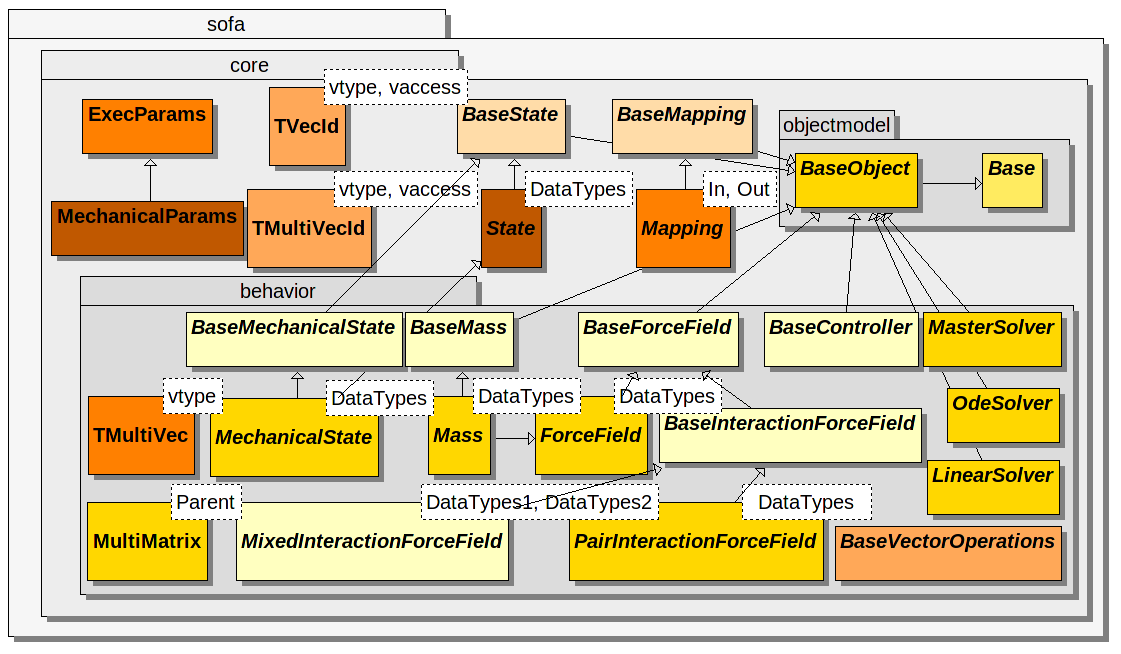
\includegraphics[scale=.33]{../classdiagrams/sofacore-behavior.png}
\caption{Classes of the \textcode{sofa::core::behavior} namespace.}
\label{fig:uml-sofa-core-behavior}
\end{figure}

\subsubsection{Changes compared to the 1.0~beta~4 version}\label{sec:design-core-behavior-changes}

\paragraph{\textcode{VecId} is replaced by templated classes to specify vector types and read/write access.}

Previously, the \textcode{VecId} class was used by solvers and visitors to specify on which state vectors should an operation be applied.
However, this API did not express the requirements for these vectors (which type, i.e. \textcode{Coord}, \textcode{Deriv}, or \textcode{MatDeriv}), nor if they were supposed to be read or written.
Now, methods and visitors can use the following classes instead (all typedefs from a common \textcode{TVecId} templated class), so that developers will now explicitly what to expect:

\begin{code_cpp}
/// Identify one vector stored in State
/// A ConstVecId only provides a read-only access to the underlying vector.
typedef TVecId<V_ALL, V_READ> ConstVecId;

/// Identify one vector stored in State
/// A VecId provides a read-write access to the underlying vector.
typedef TVecId<V_ALL, V_WRITE> VecId;

/// Typedefs for each type of state vectors
typedef TVecId<V_COORD, V_READ> ConstVecCoordId;
typedef TVecId<V_COORD, V_WRITE>     VecCoordId;
typedef TVecId<V_DERIV, V_READ> ConstVecDerivId;
typedef TVecId<V_DERIV, V_WRITE>     VecDerivId;
typedef TVecId<V_MATDERIV, V_READ> ConstMatrixDerivId;
typedef TVecId<V_MATDERIV, V_WRITE>     MatrixDerivId;
\end{code_cpp}

Also, a new class \textcode{TMultiVecId} is introduced to be able to specify different IDs for specific states or groups of states. Similar typedefs are defined as above, replacing \textcode{Vec} with \textcode{MultiVec}.

\paragraph{New State API and class hierarchy.}
The previous State API was based on \textcode{getX()}/\textcode{getV()}/... methods that returned pointers to the vectors last specified (using \textcode{setX()}/\textcode{setV()}/... methods) as the current position, velocity, ...
This is now replaced by \textcode{read(ConstVec\textit{TYPE}Id)} and \textcode{write(Vec\textit{TYPE}Id)} methods, where \textcode{\textit{TYPE}} is either \textcode{Coord}, \textcode{Deriv}, or \textcode{MatDeriv}.
These methods return a pointer to a Data instance containing the vector, instead of the vector itself.
This was necessary to respect the Data access API (see section~\ref{sec:design-core-objectmodel-changes}).
For compatibility with existing codes (especially \textcode{draw()} methods), the read-only \textcode{getX()}/\textcode{getV()}/... methods still exists but they are deprecated (and there are strictly equivalent to calling \textcode{read()} with the default ID for position, velocity, ...).
The non-const versions however are removed, so all codes modifying state vectors will have to use the new Data-based API.
Note that with this change, the state components no longer store the information about which vectors should be considered as the current position, velocity, ...
So another mechanism is required to specify these associations (\textcode{MechanicalParams}, see below).

A new state class hierarchy is also defined,  introducing a new parent class \textcode{BaseState}, common to all states (mechanical, visual, ...).
Methods allowing to read and write vectors given their IDs are specified in \textcode{State<DataTypes>}.
The \textcode{MappedModel} class is removed, non-mechanical state components (such as visual models) now directly derive from \textcode{State<DataTypes>}.


\paragraph{Simplified \textcode{Mapping} class hierarchy.}
Previously, a different base class (\textcode{Mapping< State<TIn>, MappedModel<TOut> >} or \textcode{MechanicalMapping< MechanicalState<TIn>, MechanicalState<TOut> >}) where used for mechanical versus non-mechanical (i.e. visual or one-way) mappings.
This introduced complexities and redundancies in the code of the final components (they where templated by the type of their parent class and compiled twice for each pair of input/output datatypes).
Now, a single base class is used (\textcode{Mapping<TIn,TOut>}, templated only by the input and output datatypes.
Components are also templated by the same types, similarly to other classes such as forcefields.
A new set of flags is used to check if a given mapping is mechanical or not.
Different flags are used to activate the mapping of forces, masses, and constraints separatly (although by default they have the same value).
Components that do not implement applyJT (i.e. visual mappings) can force them to false to indicate they do not support mechanical computations.

\paragraph{New mechanical component API based on \textcode{Data} and \textcode{MechanicalParams}.}
This is the most important change from the previous design.
To provide all the required vector IDs that where previously stored within each \textcode{MechanicalState} by calls to \textcode{setX()}/... methods, we define a \textcode{MechanicalParam} class.
This class is given to all mechanical-related methods, specified by \textcode{OdeSolver}s and transmitted by \textcode{MechanicalVisitor}s.
It hides the \textcode{VecId} system from most component codes, providing the same abstraction of accessing the current position and velocity vectors as was previously handled within \textcode{MechanicalState}. For example, where a component such as a \textcode{ForceField} implementation used :
\begin{code_cpp}
const VecCoord* x = this->mstate->getX();
\end{code_cpp}
It will now use \textcode{MechanicalParams} as follows :
\begin{code_cpp}
helper::ReadAccessor<VecCoord> x = *mparams->readX(this->mstate);
\end{code_cpp}

This API is preferable to directly manipulating \textcode{VecId}s (such as in \textcode{this->mstate->read(mparams->getXId(this->mstate))}) because :
\begin{itemize}
\item The code is very similar to the previous version.
\item If the API of the \textcode{VecId} or \textcode{MechanicalState} class is further changed, the \textcode{MechanicalParam::readX()} method can handle it.
\item Different \textcode{VecId}s for different states can be chosen within \textcode{MechanicalParam} (such as what is currently used for free vs mapped states, and animated vs external obstacle state).
\end{itemize}

However it is still possible to get the ids (using \textcode{mparams->x().getId(mstate)}).

All vector accesses given though \textcode{MechanicalParams} are read-only.
Vectors actually modified by each method are given as separate \textcode{MultiVecId} parameters.
This is useful to make the API clearer (we can see explicitly what each method is supposed to write) and safer (no accidental modifications to X or V within \textcode{addForce()} or \textcode{draw()} for example).
Finally, other interesting pieces of information can be queried though \textcode{MechanicalParams}.
For example, a ForceField can know as soon as the \textcode{addForce()} call if the current solver is implicit or explicit, if the kinematic and potential energy should be computed, ...

\paragraph{New solver hierarchy and vector manipulation API (\textcode{TMultiVec} and \textcode{BaseVectorOperations}).}
Previously, the solver classes had a complex hierarchy, with several parent classes (\textcode{SolverImpl}, \textcode{OdeSolverImpl}, \textcode{MasterSolverImpl}) that where used to launch each type of visitors (mechanics, linear algebra, ...).
In the new design, these classes are replaced by separate helper classes (\textcode{VectorOperations}, \textcode{MechanicalOperations}) that are instanciated at runtime and allow to launch each type of visitors while holding and updating the persistant parameters (in the form of a \textcode{MechanicalParams} for mechanical visitors for example, or \textcode{ExecParams} for simple vector operations).


\subsection{Topology (\textcode{sofa::core::topology})}

\textit{The design of this namespace is still a work in progress, so major changes should still be expected...}

\subsubsection{Changes compared to the 1.0~beta~4 version}

\textit{To be documented...}

\subsection{Collision (\textcode{sofa::core::collision})}

\begin{figure}[h]
\centering
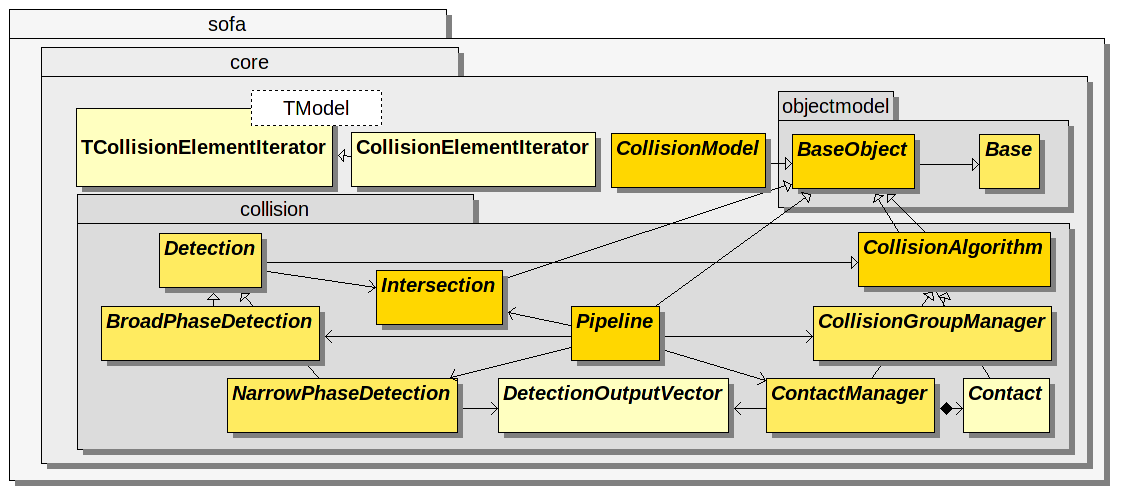
\includegraphics[scale=.33]{../classdiagrams/sofacore-collision.png}
\caption{Classes of the \textcode{sofa::core::collision} namespace.}
\label{fig:uml-sofa-core-collision}
\end{figure}

\subsubsection{Changes compared to the 1.0~beta~4 version}

\textit{No major changes.}

\subsection{Mesh and Image Loaders (\textcode{sofa::core::loader})}

\begin{figure}[h]
\centering
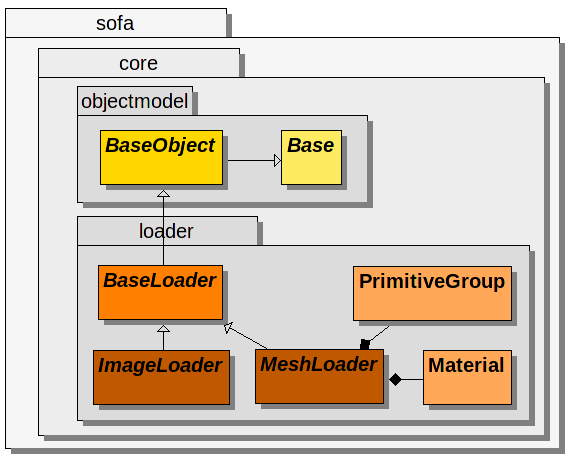
\includegraphics[scale=.33]{../classdiagrams/sofacore-loader.png}
\caption{Classes of the \textcode{sofa::core::loader} namespace.}
\label{fig:uml-sofa-core-loader}
\end{figure}

\subsubsection{Changes compared to the 1.0~beta~4 version}

This namespace is completely new.

\textit{To be documented...}

\pagebreak

\section{Main classes}

\subsection{\textcode{sofa::core::objectmodel}}

\subsubsection{\textcode{Base}}

\lstinputlisting[style=C++,linerange=51-181]{../../framework/sofa/core/objectmodel/Base.h}

\subsubsection{\textcode{BaseObject}}

\lstinputlisting[style=C++,linerange=61-160]{../../framework/sofa/core/objectmodel/BaseObject.h}

\subsection{\textcode{sofa::core}}

\subsubsection{\textcode{BaseState}}

\lstinputlisting[style=C++,linerange=39-58]{../../framework/sofa/core/BaseState.h}

\subsubsection{\textcode{State}}

\lstinputlisting[style=C++,linerange=38-103]{../../framework/sofa/core/State.h}

\subsubsection{\textcode{BaseMapping}}

\lstinputlisting[style=C++,linerange=48-116]{../../framework/sofa/core/BaseMapping.h}

\subsubsection{\textcode{Mapping}}

\lstinputlisting[style=C++,linerange=43-115]{../../framework/sofa/core/Mapping.h}


%% \section{Framework}

%% \subsection{UML Diagrams}

%% \begin{figure}[h]
%% \centering
%% 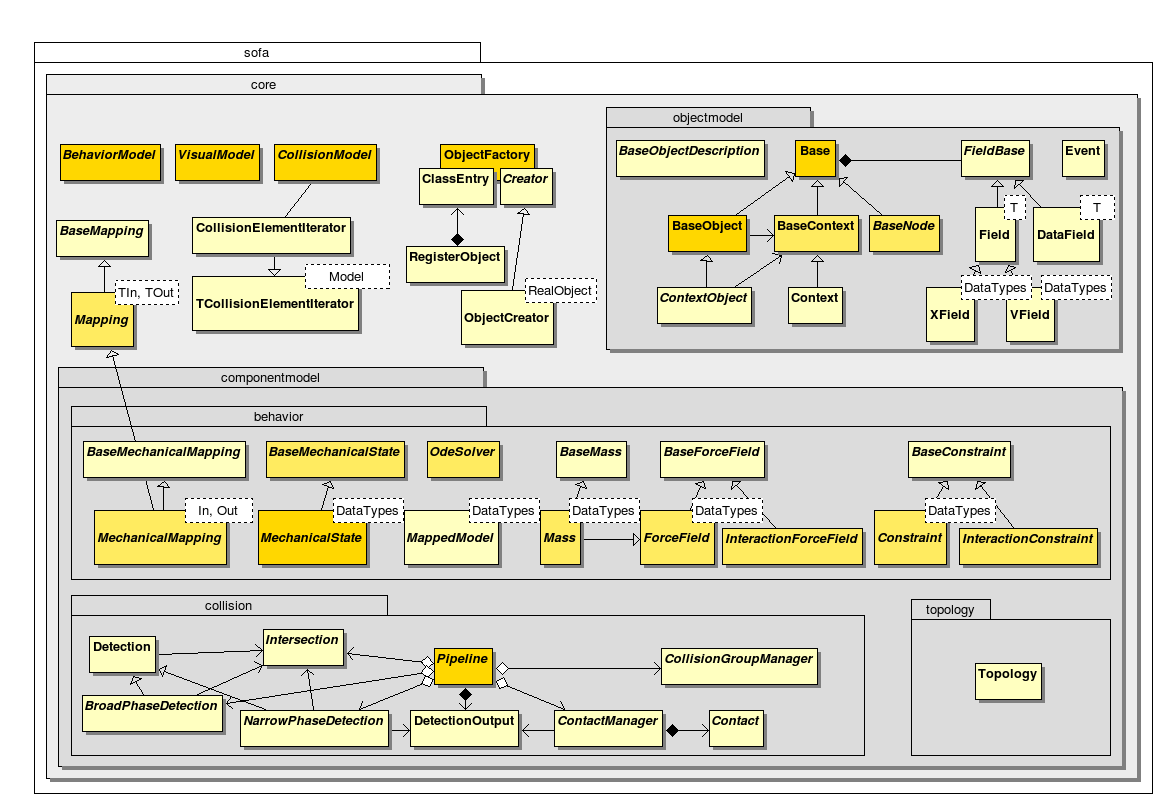
\includegraphics[width=\linewidth]{uml-sofa-core.png}
%% \caption{Classes of the sofa::core namespace.}
%% \label{fig:uml-sofa-core}
%% \end{figure}



\chapter{Modules}
\graphicspath{{../modules/}}  % to include images
In this document we explain the usage and the functionalities of the modules developped using the Core Sofa Framework.
\section{Collision Models}
\subsection{Ray Traced Collision Detection}
This module implements the algorithm described in the paper entitled "Ray-traced collision detection for deformable bodies" by E.Hermann F.Faure and B.Raffin. When two objects are in collision, a ray is shot from each surface vertex in the direction of the inward normal. A collision is detected when the first intersection belongs to an inward surface triangle of another body.  A contact force between the vertex and the matching point is then created. Experiments  show that this approach is fast and more robust than traditional proximity-based collisions.

 To speedup the  searching of elements that cross the ray,   we  stored all the triangles of each colliding objects in an  octree. Therefore we can easily navigate inside this octree and efficiently find the points crossing the ray. The octree structure allow us to have a satisfying performance independently from the size of the triangles used, which is not the case for  a regular grid.


\subsubsection{Using this module}
An example showing the usage of the Ray Traced collision detection can be found in the  RayTraceCollision.scn file in the \textit{scene} directory. The collision detection mechanism must be set as \textbf{RayTraceDetection}, and instead of using a TriangleModel one must use a \textbf{TriangleOctreeModel}. The TriangleOctreeModel will create an Octree that contains all the Triangles from the collision model. 
	


\newpage
\section{Soft Articulations}


\subsection{Concepts}

The objective of this method is to use stiff forces to simulate joint articulations, instead of classical constraints.
\paragraph{}
To do this, a joint is modeled by a 6 degrees of freedom spring. By the way, the user specify a stiffness on each translation and rotation.
\begin{itemize}
	\item A null stiffness defines a free movement.
	\item A huge stiffness defines a forbidden movement.
	\item All nuances are possible to define semi constrained movements.
\end{itemize}

\paragraph{}
2 main advantages can be extracted from this method :
\begin{itemize}
	\item A better stability. As we don't try to statisfy constraints but only apply forces, there is always a solution to resolve the system.
	\item more possibilities to model articulations are allowed. As the stiffnesses define the degrees of freedom of the articulations, a better accuracy is posssible to simulate free movements as forbidden movements, i.e. an articulation axis is not inevitably totally free or totally fixed.
\end{itemize}



\subsection{Realization}

To define physically an articulated body, we first have a set of rigids (the bones). \textsl{cf fig. 1}
\begin{figure}[hp]
	\centering
		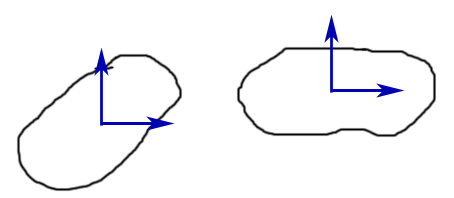
\includegraphics[width=0.30\textwidth]{softArt_G1.png}
	\caption{two bones}
	\label{2 Bones}
\end{figure}


Each of these bones contains several articulations points, also defined by rigids to have orientation information. \textsl{cf fig. 2}
\begin{figure}[htpb]
	\centering
		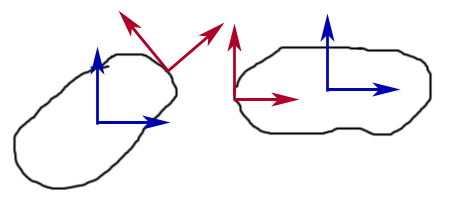
\includegraphics[width=0.30\textwidth]{softArt_G2.png}
	\caption{two bones (blue) with their articulation frames (red)}
\end{figure}

As seen previously, a joint between 2 bones is modeled by a 6-DOF spring. These springs are attached on the articulations points.    \textsl{cf fig. 3}
\begin{figure}[htpb]
	\centering
		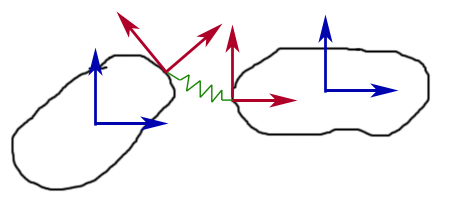
\includegraphics[width=0.30\textwidth]{softArt_G3.png}
	\caption{two bones linked by a joint-spring}
\end{figure}



\subsection{Sofa implementation}

To simulate these components in Sofa, we first need 2 mechanical objects : one for the bones (independent DOFs), and an other for the articulation points (mapped DOFs).
Each of them contains a list of rigid DOFs (respectively all the bones and all the articulations of the articulated body).
A mapping performs the link between the two lists, to know which articulations belong to which bones.


\subsubsection{Corresponding scene graph}
\begin{figure}[htpb]
	\centering
		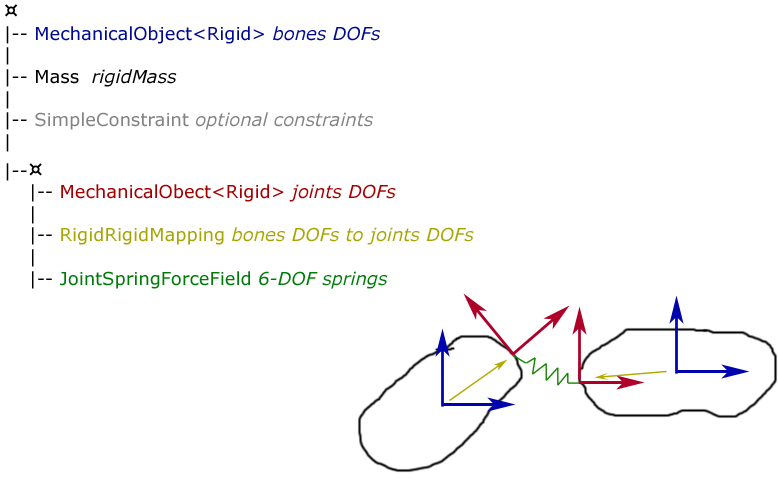
\includegraphics[width=0.90\textwidth]{scene_graph.png}
	\caption{a simple articulated body scene}
\end{figure}

\subsubsection {Example}

The example softArticulations.scn shows a basic pendulum :

\begin{verbatim}
<Node>
  <Object type="BruteForceDetection"/>
  <Object type="DefaultContactManager"/>
  <Object type="DefaultPipeline"/>
  <Object type="ProximityIntersection"/>

  <Node>
    <Object type="CGImplicitSolver"	/>
    <Object type="MechanicalObject" template="Rigid" name="bones DOFs"
            position="0 0 0  0 0 0 1 
                      1 0 0  0 0 0 1 
                      3 0 0  0 0 0 1 
                      5 0 0  0 0 0 1 
                      7 0 0  0 0 0 1" />
    <Object type="UniformMass" template="Rigid" name="bones mass"
            mass="1 1 [1 0 0,0 1 0,0 0 1]" />
    <Object type="FixedConstraint" template="Rigid" name="fixOrigin"
            indices="0" />
		
    <Node>
      <Object type="MechanicalObject" template="Rigid" name="articulation points"
              position="0 0 0  0.707914 0 0 0.707914 
                       -1 0 0  0.707914 0 0 0.707914 
                        1 0 0  0.707914 0 0 0.707914 
                       -1 0 0  0.707914 0 0 0.707914 
                        1 0 0  0.707914 0 0 0.707914 
                       -1 0 0  0.707914 0 0 0.707914 
                        1 0 0  0.707914 0 0 0.707914 
                       -1 0 0  0.707914 0 0 0.707914 
                        1 0 0  0.707914 0 0 0.707914" />
      <Object type="RigidRigidMapping"
              repartition="1 2 2 2 2" />
      <Object type="JointSpringForceField" template="Rigid" name="joint springs"
              spring="0 1   0 0 0 0 1 0   0 30000  0 200000   0  0 0 0  0 0 0 1 
                      2 3   0 0 0 0 1 0   0 30000  0 200000   0  0 0 0  0 0 0 1
                      4 5   0 0 0 0 1 0   0 30000  0 200000   0  0 0 0  0 0 0 1
                      6 7   0 0 0 0 1 0   0 30000  0 200000   0  0 0 0  0 0 0 1" />
    </Node>
    <Node>
      <Object type="MechanicalObject" template="Vec3d"
              position="-1 -0.5 -0.5  -1 0.5 -0.5 ..." />
      <Object type="MeshTopology"
              lines="0 1  1 2  ..."
              triangles="3 1 0  3 2 1  ..." />
      <Object type="TriangleModel"/>
      <Object type="LineModel"/>
      <Object type="RigidMapping"
              repartition="0 8 8 8 8" />
    </Node>
  </Node>
</Node>

\end{verbatim}

\begin{figure}[htpb]
	\centering
		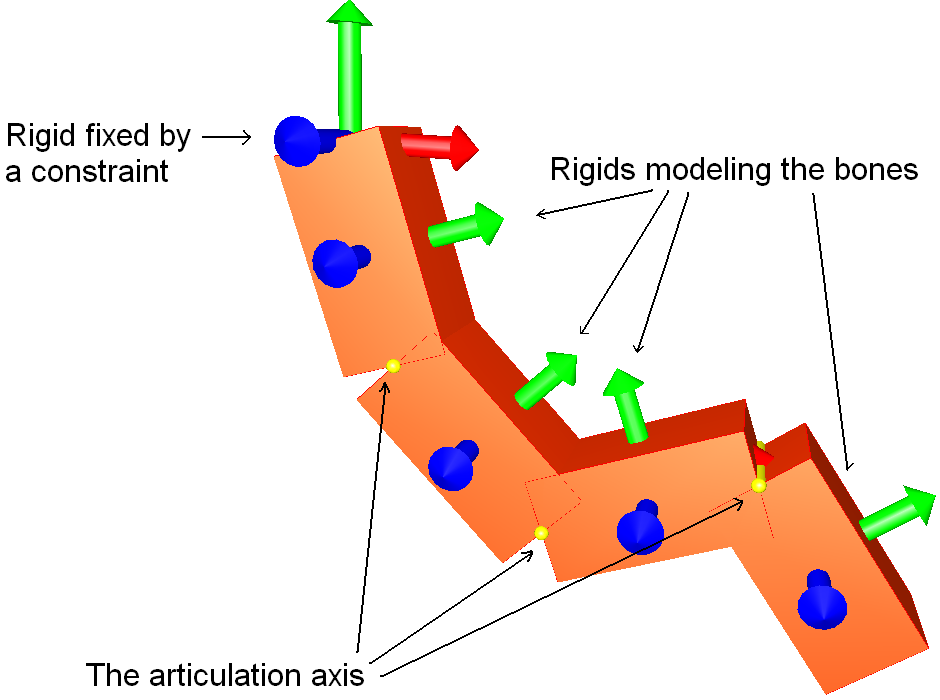
\includegraphics[width=0.70\textwidth]{softArt_snapshot.png}
	\caption{The pendulum is composed by 4 rigids linked one by one by articulations}
\end{figure}

In this example, we have under the first node the components to manage collisions, as usual.
Under the second node, we have :
\begin{itemize}
	\item the solver,
	\item the mechanical object modeling the independent rigid DOFs (5 rigids here),
	\item the rigid mass,
	\item a constraint, to fix the first rigid.
\end{itemize}

The third node (a child of the previous one) contains the components relative to the articulations :
\begin{itemize}
	\item the mechanical object modeling articulation points. Positions and orientations are relative to their parents.
	\item the mapping to link the two mechanical objects, as explained before. To know which articulations belong to which bones, a repartition vector is used. Several cases for this vector are possible :
		\begin{itemize}
			\item no value specified : every articulations belong to the first bone (classic rigid mapping).
			\item one value specified (ex: repartition="2") : each bone has the same number of articulations.
			\item number of bones values (like here, repartition="1 2 2 2 2") : the number of articulations is specified for each bone. For instance, here the first bone has 1 articulation, the next has 2 articulations, the next 2, Etc.
		\end{itemize}
	\item the JointSpringForceField containing the springs (4 springs here). Each spring is defined by a list of parameters. For instance for the first spring we have "0 1   0 0 0 0 1 0   0 30000  0 200000   0  0 0 0  0 0 0 1".
		\begin{itemize}
			\item "0 1" are the indices of the two articulations the spring is attached to
			\item "0 0 0 0 1 0" design the free axis for the movements. "0 0 0" mean that the 3 translation axis are constrained, and "0 1 0" mean that only the Y rotation axis is free.
			\item "0 30000 0 2000000" are the stiffnesses for each kind of movement: "0 30000" are respectively for free translation and for constrained translation", and "0 2000000" are respectively for free rotation and for constrained rotation.
			\item "0" is the damping factor
			\item "0 0 0" is to specify the initial translation
			\item "0 0 0 1" is to specify the initial rotation (quaternion)
		\end{itemize}
\end{itemize}

The last node contains the collision model. Nothing special here.


\subsection{Skinning}

The articulated body described previously models the skeleton of an object.
To have the external model (for the visual model or the collision model), which follows correctly the skeleton movements, it has to be mapped with the skeleton. 
\ 
A skinning mapping allows us to do this link. The external model is from this moment to deform itself smoothly, i.e. without breaking points around the articulations.

The influence of the bones on each point of the external model is given by skinning weights.
2 ways are possible to set the skinning weights to the mapping :
\begin{itemize}
	\item Either the user gives directly the weights list to the mapping. It is useful if good weights have been pre computed previsouly, like in Maya for instance.
	\item Else, the user defines a number of references \textsl{n} that will be used for mapped points. Then, each external model point will search its \textsl{n} nearest bones (mechanical DOFs), and then compute the skinning weights from the relation :
\[ W = \frac{1}{d^{2}}  \]
\small{ with \textsl{d} : the distance between the external point and the rigid DOF.}
\end{itemize}

\begin{figure*}[htpb]
		\centering
		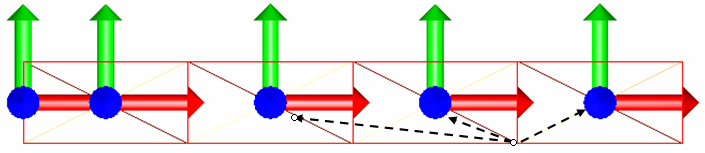
\includegraphics[width=0.50\textwidth]{skinning}
		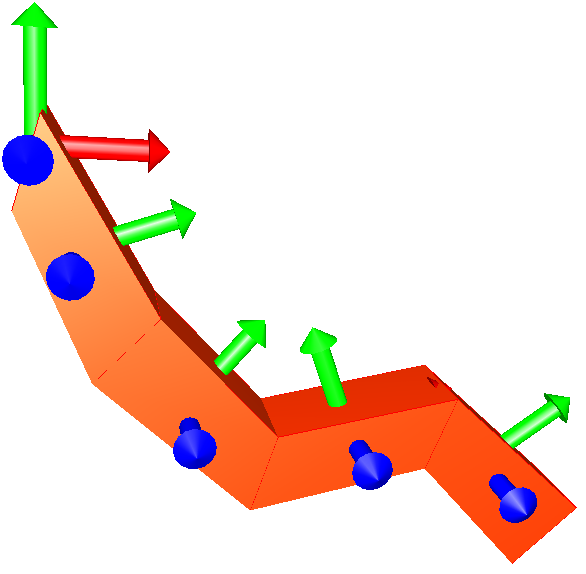
\includegraphics[width=0.30\textwidth]{skinnedPendulum}	
	\caption{In the example "softArticulationsSkinned.scn" the external points compute their skinning weights from the 3 nearest DOFs}
\end{figure*}

\newpage
\section{How to use mesh topologies in SOFA}

H. Delingette, B. Andr�

\subsection{Introduction}

\subsubsection{BTW, What is a mesh topology ?}

A mesh is usually described as a set of points that are connected by
edges, triangles or any other type of mesh element. Thus it is
useful to make a clear a distinction between two different aspects
of a mesh :

\begin{itemize}

 \item \textbf{Mesh Geometry} : the mesh geometry consists in the position of the mesh vertices.
This information depends on the space where the mesh in embedded.
For instance in a 2D triangulation, each vertex position is a 2D
vector while in a 3D triangulation, each vertex position is a 3D
vector. Therefore the mesh geometry can be described as an array of
vector whose size is the number of mesh vertices. In SOFA, we use
the word Degree Of Freedom (DOF) to describe such an array because
it can be used to store other geometric information (rigid
transformation, first or second derivatives, etc.).

 \item \textbf{Mesh Topology} : the mesh topology describes how the vertices are
connected with each other. For instance, it describes the set of
triangles by specifying the 3 vertex indices that make each
triangle. A mesh topology manipulates vertex indices (as unsigned
int) and therefore is independent of the embedding space. For
instance, a 2D and a 3D triangulation may have the same mesh
topology but with different mesh geometry.

\end{itemize}


\subsubsection{Why do I need to bother with mesh topologies ?}

As discuss above, mesh topology is an essential part of a mesh and
therefore any computation task that requires a mesh needs to know
how to use a mesh topology.\\ This includes:

\begin{itemize}

 \item \textbf{Mesh Visualization},

 \item \textbf{Collision detection} : some collision detection are mesh based (e.g.
triangles or edges),

 \item \textbf{Mechanical Modeling} : deforming a mesh also requires to the
knowledge of a mesh topology. For instance a spring mass model
requires knowing about the edges that connects pair of vertices,

 \item \textbf{Haptic rendering},

 \item \textbf{Description of scalar} (temperature, electric potential, etc.) or
vectorial fields (speed, fiber orientation, etc.)

\end{itemize}

Using a mesh topology is relatively simple since it consists in
having access to arrays of indices corresponding to vertex indices
or edge indices or other topological items.
\\

A more tricky part consists a) in changing locally or globally this
topology (adding a triangle, removing an edge) and b) in propagating
those changes to all objects using the mesh topology to perform a
task (visualization, deformation, etc.)

\subsubsection{How are Mesh Topologies designed in SOFA ?}

The mesh geometry in SOFA is stored in a MechanicalObject which is a
template class because it depends on the embedding space (2D or 3D
Euclidian space), the vector class and the required floating point
accuracy (float vs double).
\\

A mesh topology is stored in a different object than the mesh
geometry.
\\

One important aspect of the design of mesh topologies in SOFA is the
fact that they are organized in a class hierarchy. For instance, a
triangulation object derives from an edge set object since a
triangulation can be also viewed as a set of edges, each triangle
having 3 edges. This is very important to design generic software
components. Indeed, following the same example, with this design, a
spring mass mechanical model that only requires the knowledge of
edges (pairs of vertices) can also be used on a triangulation or any
other mesh (quad, hexahedral, tetrahedral mesh)  that derives from
an edge set object.
\\

Another interesting feature in SOFA is the ability to provide
multiple topology descriptions for the same mesh. For instance a
quad element (see figure below) has four DOFs which can be connected
with 2 triangles or 6 edges. Thus, the same mesh geometry can be
described by 3 different mesh topologies. SOFA uses the mechanism of
topological mapping to provide multiple topologies associated with
the same mesh geometry. Those mappings also apply to map a subset of
the mesh topology into a new mesh topology.  For instance the border
of a tetrahedral mesh can be mapped into triangulation mesh or edges
of a triangulated mesh can be mapped into a polygonal mesh.\\


\begin{figure*}
 \centering
 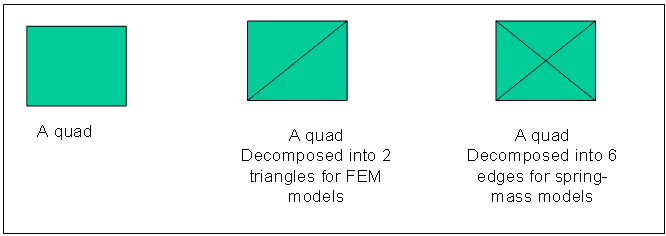
\includegraphics[width=0.95\linewidth]{Quad_Multiple_Topologies}
  \caption{Multiple topology descriptions of the Quad.}
 \label{fig:Quad_Multiple_Topologies}
\end{figure*}

Another important aspect of the design is the fact that topological
changes (mesh cutting or refinement) are handled in SOFA.  For the
programmer, it implies that specific containers must be used to
store data for each software component. For instance, a spring mass
model must store the spring stiffness of each edge. Therefore the
container of spring stiffness must have the same size than the
number of edges in the mesh. In SOFA, to cope with topological
changes that can add or remove the number of edges, it is mandatory
to use a specific container (in such case EdgeData container) that
will automatically resize itself when topological changes occur.

\subsubsection{What are the different mesh topologies supported in SOFA ?}


\subsection{Using Mesh Topologies}

\subsubsection{What is a mesh topology object ?}
\subsubsection{What is the difference with the old MeshTopology object ?}
\subsubsection{What are the different mesh topology objects in SOFA ?}


\begin{figure*}
 \centering
 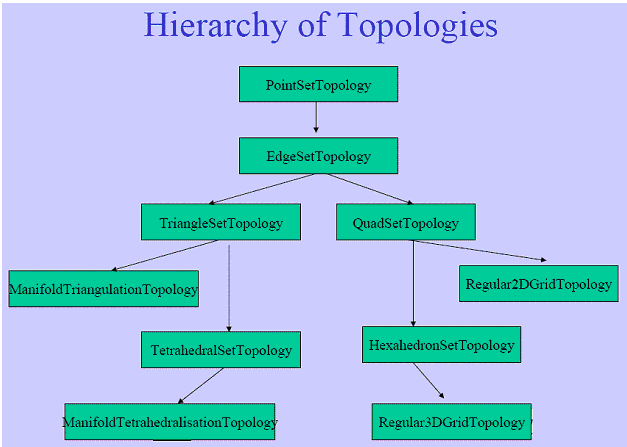
\includegraphics[width=0.95\linewidth]{Hierarchy_Topologies}
  \caption{A generic and hierarchical topology is described from a class called BaseTopology.}
 \label{fig:Hierarchy_Topologies}
\end{figure*}

BaseTopology class provides an implementation which handles
topological changes, full topological relationships and geometric
computation.

\subsubsection{How do I have access to the adjacency information between items ?}
\subsubsection{What to do if I need to know only basic topology information ?}
\subsubsection{What are the geometry algorithms stored in each topology classes ?}

\subsection{Handling Topological Changes}

\subsubsection{How does it work ?}
\subsubsection{What container should I use to handle the topology changes ?}
\subsubsection{How to write the different callback functions associated with the containers ?}

Topological changes are handled in a way which is as much
transparent for the user as possible.


\subsubsection{The 4 components of a BaseTopology object}

\begin{verbatim}

Class BaseTopology<DataTypes> {

// A container for info to be stored and methods to access adjacency :
//   - Adjacency Information is only computed when needed
//   - Non template class
//   - Store TopologicalChange list

TopologyContainer *container ;

// A modifier for low-level methods to change topology :
//   - Cannot be accessed from user
//   - Modifier also changes the DOFs in the Mechanical Object
//   - Low level methods to add or to remove an item
TopologyModifiers<DataTypes> *modifier ;

// TopologyAlgorithms for high-level methods to change topology (user access) :
//   - Accessed from the user
//   - High level algorithms to refine, cut mesh
TopologyAlgorithms<DataTypes> *topologyAlgorithms ;

// Geometry Algorithms methods to get geometry information :
//   - Compute geometric information (normal, curvature, area, length)
GeometryAlgorithms<DataTypes> *geometryAlgorithms ;

};

\end{verbatim}


\subsubsection{Implementation for objects inherited from each other (Point,
Edge, Triangle, Tetrahedron}


\begin{itemize}

 \item PointSetTopology (inherited from BaseTopology) :

    \begin{itemize}

    \item Container : For each point gives its global index. This is useful for subset topologies (subset triangulation, ...) where the number of vertices involved in the topology may not be the same as the total number of vertices.

    \item Modifier : addPointsProcess, removePointsProcess, renumberPointsProcess, addPointsWarning, removePointsWarning, propagateTopologicalChanges

    \item Geometry : computeCenter, computeRadius,
    getAABB()

    \end{itemize}


\item EdgeSetTopology (inherited from PointSetTopology)

    \begin{itemize}

    \item Container : array of edges, array of vertex-edge shell

    \item Modifier : addEdgesProcess, removeEdgesProcess, fuseEdgesProcess, splitEdgesProcess,
   addEdgesWarning, removeEdgesWarning

    \item Geometry : getEdgeLength, getRestEdgeLength

    \end{itemize}


\item TriangleSetTopology (inherited from EdgeSetTopology)

    \begin{itemize}

    \item Container : array of triangles, of vertex- and edge-triangle shell

    \item Modifier : addTrianglesProcess, removeTrianglesProcess, addTrianglesWarning, removeTrianglesWarning

    \item Topology Algorithms : InciseAlongPointsList, RemoveAlongTrianglesList

    \item Geometry : computeTriangleNormal

    \end{itemize}


\item TetrahedronSetTopology (inherited from TriangleSetTopology)

    \begin{itemize}

    \item Container : array of tetrahedra, array of vertex-, edge-, triangle-tetrahedra shell

    \item Modifier : addTetrahedraProcess, removeTetrahedraProcess, addTetrahedraWarning, removeTetrahedraWarning

    \item Geometry : computeTetrahedronVolume

    \end{itemize}

\end{itemize}

\begin{figure*}
 \centering
 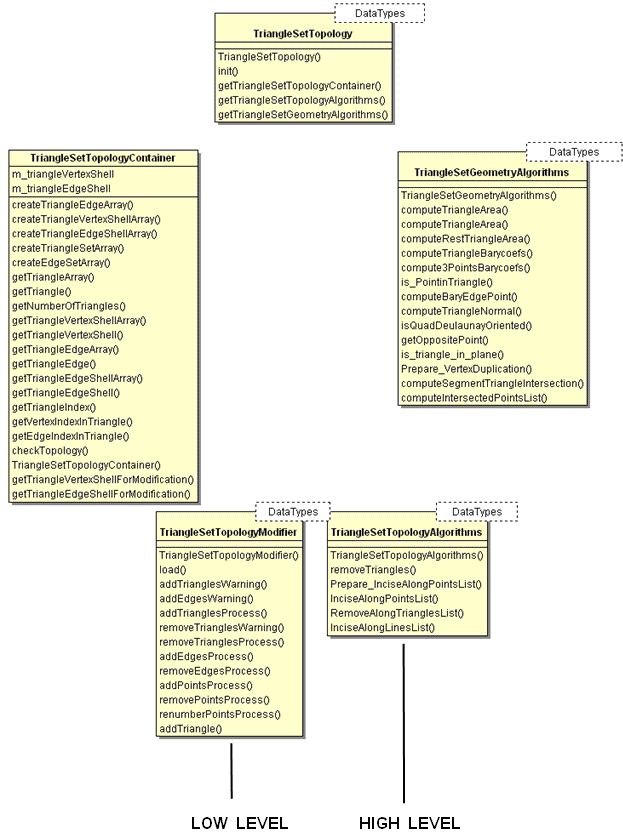
\includegraphics[width=0.95\linewidth]{UML_TriangleSetTopology}
  \caption{UML diagram describing the 4 components of TriangleSetTopology class.}
 \label{fig:UML_TriangleSetTopology}
\end{figure*}

\newpage

\begin{figure*}
 \centering
 \includegraphics[width=0.95\linewidth]{UML_BaseTopology}
  \caption{UML diagram showing the use of a TopologyChanges List from BaseTopology class.}
 \label{fig:UML_BaseTopology}
\end{figure*}

\newpage

\subsubsection{Definition of data structures to be "aware" of topological
changes}

Force Fields, Constraints, Mapping and other modules may require to
store information for each topological item (point, edge, triangle,
etc.).
\\

Two container data structures are defined to handle topological
changes by matching the types of TopologyChanges :

\begin{itemize}

    \item PointData$<$MyType$>$, EdgeData$<$MyType$>$ are arrays (same as std::vector) of item of type MyType

    \item PointSubset, EdgeSubset are arrays of points or edges

\end{itemize}

Used-defined functions are called when an item is created or
destroyed.
\\

In higher level classes (for example
TriangularQuadraticSpringForceField, DiagonalMass or FixedConstraint
classes), the user only provides callback functions to handle :

\begin{itemize}

    \item the creation of a topological item
    \item the destruction of a topological item

\end{itemize}

\begin{figure*}
 \centering
 \includegraphics[width=0.95\linewidth, height=0.95\textheight]{UML_Topological_Changes}
  \caption{These UML diagrams show the use of EdgeData, PointData and
PointSubset to handle topological changes implying modifications
respectively in ForceField, Mass and Constraint modules.}
 \label{fig:UML_Topological_Changes}
\end{figure*}

\newpage

\begin{figure*}
 \centering
 \includegraphics[width=0.95\linewidth]{Order_Notifications}
  \caption{Order to respect when adding or removing an item (see the
explanations in the following example).}
 \label{fig:Order_Notifications}
\end{figure*}

\begin{itemize}

    \item "WARN" means : add the current topological change (add or delete a list of items) in the list of TopologyChanges

    \item "PROPAGATE" means :  traverse the simulation tree with a TopologyChangeVistor to send
    the current topological change event to all force fields, constraints,
    mappings, etc.

\end{itemize}

\subsubsection{Example : What happens when I split an Edge ?}

\begin{figure*}
 \centering
 \includegraphics[width=0.95\linewidth]{Topology_Example_1}
 \includegraphics[width=0.95\linewidth]{Topology_Example_2}
  \caption{What happens when I split an Edge ? - Step 1. 2.}
 \label{fig:Topology_Example_12}
\end{figure*}

\newpage

\begin{figure*}
 \centering
 \includegraphics[width=0.95\linewidth]{Topology_Example_3}
 \includegraphics[width=0.95\linewidth]{Topology_Example_4}
  \caption{What happens when I split an Edge ? - Step 3. 4.}
 \label{fig:Topology_Example_34}
\end{figure*}

\newpage

\begin{figure*}
 \centering
 \includegraphics[width=0.95\linewidth]{Topology_Example_5}
 \includegraphics[width=0.95\linewidth]{Topology_Example_6}
  \caption{What happens when I split an Edge ? - Step 5. 6.}
 \label{fig:Topology_Example_56}
\end{figure*}

\newpage

\begin{figure*}
 \centering
 \includegraphics[width=0.95\linewidth]{Topology_Example_7}
 \includegraphics[width=0.95\linewidth]{Topology_Example_8}
  \caption{What happens when I split an Edge ? - Step 7. 8.}
 \label{fig:Topology_Example_78}
\end{figure*}

\newpage

\begin{figure*}
 \centering
 \includegraphics[width=0.95\linewidth]{Topology_Example_9}
  \caption{What happens when I split an Edge ? - Step 9.}
 \label{fig:Topology_Example_9}
\end{figure*}


\newpage
\section{Graphic User Interface}
\subsection{First steps}
\par
Once SOFA is compiled, in the directory bin will be placed an executable called runSofa (or runSofad if you are using the debug version).
The first time you will run SOFA, a GUI using Qt will appear. By default a simulation modeling a liver with some fixed points will be displayed. Simulations must be written in a xml format, generally, Sofa scenes have the extension ``.scn'', and Sofa objects directly the extension ``.xml''. You can load both of them using the file menu, or drag \& dropping them in the interface.\\
Basically the GUI is divided in two: 
\begin{itemize}
 \item a control panel subdivided in several tabulations, giving the user the possibility to display various information about the simulation, and even modifying it interactively
 \item a viewer: by default, you will be using our hand-made viewer, using OpenGL. Others are available, and below, we describe how to create your own viewer, if you desire to insert a more powerful rendering engine.
\end{itemize}

\begin{figure}[htpb]
	\centering
		\includegraphics[width=1.0\textwidth]{GUI/GUI.png}
	\caption{SOFA first-time}
\end{figure}
At any time, you can hide the control panel by moving its right border to the left.
\newline

\par

\begin{figure}
	\centering
		\includegraphics[width=0.45\textwidth]{GUI/GUI_basic.png}
	\caption{Basic Controls}
\end{figure}\begin{center}

\vspace{25mm}            \end{center}
The basics controls are :
\begin{itemize}
 \item {\bf Animate} : launch the simulation. The simulation won't stop until you press Animate.
 \item {\bf Step}: Process only one step of the simulation. 
 \item {\bf Reset Scene}: Reset all the components to their initial values.
 \item {\bf Reset View}: Reset the camera to its original place.
 \item {\bf Save View}: Save the position and orientation of the camera. Next time you will load your scene, these information will be used.
 \item {\bf Save Caption}: Take a screenshot of the current simulation.
\end{itemize}

DT corresponds to the time step used in the computation of the simulation. It can be changed interactively.










\subsection{View Tab}
The ``View Tab'' is the default tab, you can filter the information you want to be displayed by your viewer. It is quite useful to have a fast and global control. 

\begin{figure}[htpb]
	\centering
		\includegraphics[width=0.3\textwidth]{GUI/GUI_visual.png}
	\caption{Basic Controls}
\end{figure}

The options are:
\begin{itemize}
 \item {\bf All}: Enable or disable the display of all the visual information available in SOFA
 \item {\bf Visual Models}: the graphic representation of the objects
\item {\bf Behavior Models}: the mechanical DOFs of the simulation
\item {\bf Collision Models}: the models used to perform the collision detection
\item {\bf Bounding Tree}: the hierarchical bounding boxes of the collision models
\item {\bf Mappings}: All the non-mechanical mappings (for instance the visual mappings that link a mechanical object to its visual representation)
\item {\bf Mechanical Mappings}: All the mechanical mapping that propagates the forces and position from a mechanical object to another
\item {\bf Interactions}: Interactions of all kind between objects. Some are created by the collision pipeline when a penalty response is used
\item {\bf Wire Frame}: Change the way 3D models(visual, and collision) are displayed
\item {\bf Normals}: Normals of the visual models
\end{itemize}








\subsection{Stats Tab}
The ``Stats Tab'' is a tab displaying an inventory of the collision models present in the scene( how many triangles, lines, points, spheres, are used to perform the collision detection). You can also output some information about the current simulation. 
\begin{itemize}
 \item Dump State: export in ``dumpState.data'' the state of the simulation
 \item Log Time: display in the console, the time spent in each step of the simulation. Useful to do some monitoring
 \item Gnuplot: export gnuplot files. It will export positions, velocities, energies. Files will have the same name as the Object associated in the simulation, following by:
\begin{itemize}
 \item {\bf ``\_x''} for the positions
 \item {\bf ``\_v''} for the velocities
 \item {\bf ``\_Energy''} for the Energies (contains kinetic, potential and mechanical)
\end{itemize}

You can specify the directory where you want the files to be saved in the menu Edit.
\end{itemize}











\subsection{Graph Tab}
The ``Graph tab'' is certainly the most important tab. It displays the scene graph of the simulation. You can quickly see all the components used in the current simulation. The ``Export Graph...'' button gives a graphic representation of the inter-dependencies of the objects.

\begin{figure}[htpb]
	\centering
		\includegraphics[width=0.5\textwidth]{GUI/GUI_graph.png}
	\caption{Scene Graph for the liver scene}
\end{figure}

This graph can dynamically change during the simulation: collisions can create new nodes, new components in case of contacts. But you can directly interact with it too. Double clicking on an item of the graph will make appear a small window displaying important data.

To know how to display the information of your brand new Sofa component, please refer to the section ``How to configure your Component''. Only objects of type ``sofa::core::objectmodel::Data'' or ``sofa::core::objectmodel::DataPtr'' can be displayed. It is important to understand that only these information will be kept if you decide to save the simulation. Loading a saved simulation, will just fill the components with this data.
This kind of dialog windows give the possibility to modify directly some characteristics of your component. Take care to click on the button ``Update'' once you have completed your modifications.

\begin{figure}[htpb]
	\centering
		\includegraphics[width=0.8\textwidth]{GUI/GUI_modify.png}
	\caption{Double click on an item of the graph}
\end{figure}

\par
A Node gives access to much more interactions: right clicking on one of them makes appear a small context window.
\begin{itemize}
 \item {\bf Collapse}: Collapse the graph from the current node, close all the nodes below the clicked one
 \item {\bf Expand}: Expand the graph, and open all the nodes below the clicked one
 \item {\bf Desactivate}: Deactivate a part of the scene. Everything below this node won't be anymore taken into account. BUT it remains in the scene, and can be Activated again at any time
 \item {\bf Save Node}: Export in a XML files a part of the simulation
 \item {\bf Add Node}: Read a XML files describing an object or a whole scene, and put it right below the clicked node.
An interesting feature to note, is when you might be always using, and adding the same set of objects, you will find it convenient to add in the file scenes/object.txt the path to them. Like this, they will directly appear in the dialog window by default.
 \item {\bf Remove Node}: Remove from the simulation everything within the clicked node. You won't be able anymore to make it appear unless you proceed to a restart or reload of the scene.
 \item {\bf Modify}: Open the same dialog window as might do a double click: this action is common to all the items of the graph
\end{itemize}

\begin{figure}[htpb]
	\centering
		\includegraphics[width=0.4\textwidth]{GUI/GUI_interaction.png}
	\caption{Right click on a node of the graph}
\end{figure}








\subsection{Viewer Tab}
The ``Viewer tab'' describes all the keyboard shortcuts available for the current viewer.

The last useful option of this tab is the possibility to re-size your viewer, which can be very helpful to record a video at a given resolution.









\subsection{Interactions}
You can interact with the simulation using the mouse with SHIFT + Right Click. A ray will be cast, and if it intersects one collision model of the scene, a spring will be created, allowing you to pull on some elements of the scene.



\newpage
\subsection{Architecture}
Fig.~\ref{fig:GUI_UML} gives an overview of the modular architecture of the GUI for SOFA. 
\begin{figure}[htpb]
	\centering
		\includegraphics[width=0.9\textwidth]{GUI/GUI_UML.png}
	\caption{A modular Architecture of the GUI}
 	\label{fig:GUI_UML}
\end{figure}








\subsection{Change the viewer}
By default, SOFA provides three viewers, that can be integrated easily to the Qt interface. 

\begin{itemize}
 \item {\bf QtViewer}: a hand made viewer using OpenGL functionality
 \item {\bf QtGLViewer}: a viewer using the library QGLViewer created by Gilles Debunne. It is distributed directly with SOFA, but you can also download it at:\\ {\bf http://artis.imag.fr/Members/Gilles.Debunne/QGLViewer/}
 \item {\bf OgreViewer}: this viewer remains experimental, but shows how it is possible to integrate a powerful rendering engine such as OGRE3D. You need to install Ogre. You can download it at {\bf http://www.ogre3d.org}.
\end{itemize}

To use them, you have to edit the file sofa-default.cfg located in your SOFA directory, and uncomment the lines corresponding to the viewer you want. If you have several viewers activated, you can launch SOFA with a specific one by using the option:
\begin{itemize}
 \item ``runSofa -g qt'' : for QtViewer
 \item ``runSofa -g qglviewer'' : for QtGLViewer
 \item ``runSofa -g ogre'' : for OgreViewer
\end{itemize}

You can also dynamically change the viewer when SOFA is running. The menu View of the main window displays all the viewer available and let you switch at any time.
\par
If you desire to create a new viewer, the first step is to make it derive from SofaViewer. 








\subsection{Choose the GUI}
By default, Sofa provides three GUIs.
\begin{itemize}
 \item {\bf Batch}: no gui, proceeds to 1000 iterations and then stops
 \item {\bf GLUT}: GLUT window, implementing only the basic functions. To start the animation, you have to pass the option ``-s'' to your runSofa
 \item {\bf Qt}: the default GUI, already described above
\end{itemize}

The Batch GUI is always available. To use GLUT or Qt interface, you have to uncomment in sofa-default.cfg the corresponding lines. To use them
\begin{itemize}
 \item ``runSofa -g batch'' : for no GUI
 \item ``runSofa -g glut'' : for GLUT window 
 \item for Qt GUI, please refer to the section above. By default, Sofa is using Qt interface with QtViewer.
\end{itemize}
If you desire to create a new GUI, the first step is to make it derive from SofaGUI. 






\subsection{Player/Recorder}

\begin{figure}[htpb]
	\centering
		\includegraphics[width=0.7\textwidth]{GUI/GUI_recorder.png}
	\caption{Player/Recorder in Sofa} 	
\end{figure}
Sofa provides with the Qt Graphic interface, a compact Player/Recorder of simulation. When you want to record a simulation, press the red button (record). Automatically, some components will be added to your graph, and will create files to save the position, and velocities of all your mechanical elements. To stop recording, press again on the record button. A file with the same name as your simulation will be created, but with the extension ``.simu''. Sofa is able to read these files, and will initialize correctly the Player. 
\par
To readback a recorded simulation, you can process to a step by step(forward, and backward), or a continuous play. You can jump to a specific moment of your recording. You can even change the Dt of the recording, if you want to accelerate, or reduce the velocity of the playing. At any time, you can animate the scene (by pressing the Animate button), to compute the simulation. 
\par
The files will be stored by default in the directory scenes/simulation of your SOFA. Nevertheless, you can change this directory by clicking on the menu Edit of the main window.







\section{Modeler}
A modeler for Sofa has been recently created. The purpose of this tool is both to help the new-comers in Sofa to get an overview of the whole framework, and accelerate the process of creation and configuration of a complex simulation for expert users.
\begin{figure}[htpb]
	\centering
		\includegraphics[width=0.75\textwidth]{GUI/Modeler.png}
	\caption{Main Window of the Modeler} 	
\end{figure}

\subsection{Library}
The left part of the application displays a library of all the different components available in Sofa, sorted by the name of the Base Class. Clicking on any of them will display information about the usage, authors, licence if any, and sometimes a link to an example. This link will open a new tab in the modeler displaying a simulation. 
At any time, you can launch Sofa from the Modeler, hitting CTRL+R, or going to File ... Run In Sofa.
\subsection{Graph Editor}
The right part seems very similar to the scene graph displayed in Sofa. The behavior is the same. Double clicking on a component will open a dialog, in which you can define all the parameters of the object. But, as you are in an editor, you can easily remove everything you have added. This editor is very convenient to test things. Try to create your object, launch into sofa, modify some components, or parameters, using the documentation displayed each time you select one item. 
\subsection{Modeling}
To model a new scene, just make a series of drag and drop of the components you desire from the Library to the Graph Editor. By default, when opening a new tab, all the default components to perform the collision detection are added. If you don't want them, just clear the tab (CTRL+N).\\
To accelerate the process of creation, preset objects are available. You can build automatically :
\begin{itemize}
  \item deformable objects
  \begin{itemize}
    \item in a grid
    \item using a tetrahedral mesh
  \end{itemize}
  \item rigid objects  
  \begin{itemize}
    \item simulated
    \item not simulated: they will perform as obstacle like floors, or walls
  \end{itemize}
\end{itemize}



\newpage

\section{Light management}

One white global light illuminates the scene by default. This can be changed
through a light manager object and a certain number of lights (limited by
OpenGL).

The first step is to add the object called ``LightManager'', preferably at the
top of the scene file.
\begin{code_xml}
	<Object type=``LightManager'' />
\end{code_xml}

After that, we can add 3 different kinds of lights :
\begin{itemize}
  \item a positional light (parameters : color, position) ;
	\begin{figure}[!h]
	\centering
	\includegraphics[width=0.33\linewidth]{rendering/images/light_pos.png}
	\caption{Positional Light}
	\end{figure}

	\begin{code_xml}
		<Object type="PositionalLight" position="0 -5 10" />
	\end{code_xml}
%\newpage
  \item a directional light (parameters : color, direction) ; 
	\begin{figure}[!h]
	\centering
	\includegraphics[width=0.33\linewidth]{rendering/images/light_dir.png}
	\caption{Directional Light}
	\end{figure}

	\begin{code_xml}
		<Object type="DirectionalLight" direction="0 5 0" />
	\end{code_xml}
\newpage

  \item and a spotlight (parameters : color, position, direction, cut off,
  exponent, attenuation)

	\begin{figure}[!h]
	\centering
	\includegraphics[width=0.33\linewidth]{rendering/images/light_spot.png}
	\caption{Spot Light}
	\end{figure}

	\begin{code_xml}
		<Object type="SpotLight" position="-3 2 5" direction="0 0 -1" />
	\end{code_xml}
\end{itemize}

\section{Shader management}
A complete set of tools about using shaders is implemented into SOFA. The three kinds of shaders (vertex and fragments (mandatory), geometry (optionally)) are available.
Shader is used only for Visual Model as OglModel.
\newline
The effects of the shader is spread to the associated subtree.
Finally, there is only one shader activated for each visual model : if two shaders are present in the same node, only the second will be effective.

	\begin{figure}[!h]
	\centering
	\includegraphics[width=0.8\linewidth]{rendering/images/shader_tree.png}
	\caption{Example of shaders' area of effect}
	\end{figure}

To simply include a shader, add this into your node :
	\begin{code_xml}
		<Object type="OglShader" vertFilename=``test.vert'' fragFilename=``test.frag'' />
	\end{code_xml}

\textit{vertFilename} and \textit{fragFilename} are the only mandatory parameters. Other optional parameters are about geometry shader : \textit{geoFilename}, \textit{geometryInputType}, \textit{geometryOutputType} and \textit{geometryVerticesOut}. A last parameter, \textit{turnOn}, is for debugging purpose, when you want to disable shader without restarting the scene.

If you want to send values to uniform varaibles defined into the shader, a certain number of objects is available : 
\begin{itemize}
 \item OglIntVariable,OglInt{2,3,4}Variable : for int and ivec{2,3,4}
 \item OglFloatVariable,OglFloat{2,3,4}Variable : for float and vec{2,3,4}
 \item OglIntVectorVariable, OglIntVector{2,3,4}Variable : for arrays of int and ivec{2,3,4}
 \item OglFloatVectorVariable, OglFloatVector{2,3,4}Variable : for arrays of float and vec{2,3,4}
\end{itemize}

Their parameters are \textit{id} for their name into the shader and \textit{value} (single type) or \textit{values} (array type).
Example : 
	\begin{code_xml}
		<Object type="OglFloat3Variable" id="fragmentColor" value="1.0 0.0 0.0" />
		<Object type="OglFloatVariable" id="fragmentOpacity" value="2.0"/>
		<Object type="OglFloatVector4Variable" id="MappingTable" values="1.0 0.0 0.0 0.0 0.0 0.0 0.0 1.0" />
	\end{code_xml}

2D texture can be added with OglTexture2D object.Its parameters are \textit{id}, \textit{texture2DFilename} and \textit {textureUnit}.

	\begin{code_xml} 
		<Object type="OglTexture2D" texture2DFilename="textures/lights4-small-noise.bmp" textureUnit="1" id="planeTexture" />
	\end{code_xml}

The last object about shaders is a partial support of macro processing in GLSL. It's possible to define macro variable if a part of code is enabled or not. For example, this can be very useful if there is a common code for two 3D objects, one with a texture, and the other with simple colors. You define the macro :

	\begin{code_cpp} 
		#define HAS_TEXTURE
			...;
			//code about textured 3D object
		#else
			...;
			//code about colored 3D object
		#endif
	\end{code_cpp}

and put the following object into the scene file, at the same node as the OglShader used by the textured 3D object:

	\begin{code_xml} 
		<Object type="OglShaderDefineMacro" id="HAS_TEXTURE" />
	\end{code_xml}





\part{Practical guide}

\chapter{How To}
\graphicspath{{../HowTo/}}  % to include images
In this document we will try to give small tutorials on various topics you should encounter during your experience with SOFA.

\section{How To create a simulation}
To create your own simulation, from a xml description, or a c++ file, you have to respect some rules.
The Modeler can be used to have a quick view of all the components already available in Sofa.
\subsection{Model a dynamic object}
To model a dynamic object, you have to follow that steps:
\subsubsection{Mechanical}
\begin{enumerate}
 \item { \bf GNode}: Generally, we give it the name of the whole object
 \item { \bf Solver}: choose the solver you want to resolve this part of the simulation (you might need two components actually, a OdeSolver followed by a LinearSolver)
 \item { \bf Topology}: describes how the dofs will be connected
 \item { \bf MechanicalState}: the degrees of freedom (dofs) of your object. It is the heart of the simulation
 \item { \bf Mass}: the mass attached to each dofs of the object
 \item { \bf ForceField}: describes the behavior of your object, how it will interact. If you don``t specify one, your model won't be deformable
 \item { \bf Constraint}: optional
\end{enumerate}

\begin{figure}
	\centering
		\includegraphics[width=0.5\textwidth]{Modelling0.jpg}
	\caption{Basic example modelling a Finite Element Object}
\end{figure}
After these steps, you will have a mechanical model, that can be integrated in a Sofa Simulation. Nevertheless, you won't have any visual model, only points representing your dofs.


\subsubsection{Visual}
Using the previously described mechanism of Mapping, you can attach a visual model, of any kind, to represent your mechanical object.

\begin{enumerate}
 \item { \bf GNode}: add a GNode inside your current object. It will contain the components necessary to do the visual mapping
 \item { \bf VisualModel}: this component contains the mesh representing your object
 \item { \bf Mapping}: a non-mechanical mapping will connect your mesh to the dofs. This mapping won't transmit forces from your visual model to the dofs. If you are writting...
\begin{itemize}
 \item { \bf a c++ file}, take good care of using a non-mechanical template: The second object should be a template of ExtVec3Types
 \item { \bf a xml file}, you have to specify the path to the two models to be mapped: 
\begin{itemize}
 \item object1=''../..`` : meaning the dofs are located one level below
 \item object2=''Visual`` : where ''Visual'' is the name of your VisualModel (as described in this example, it is located at the same level as your mapping)
\end{itemize}
\end{itemize}
 
\end{enumerate}

\begin{figure}[htpb]
	\centering
		\includegraphics[width=0.5\textwidth]{Modelling1.jpg}
	\caption{Basic example modelling a Finite Element Object with a Visual Model}
\end{figure}
\subsubsection{Collision}
If you need to simulate interactions between objects, you will need another node, a Collision Node.
In the example we describe, we will use a Triangle Model as collision model. We chose it because, it behaves like most of our collision models, needing a topology and dofs to behave properly. But if you use the simple SphereCollisionModel, this component already contains a topology, dofs and collision model. So you will just have to create a mechanical mapping.
\begin{enumerate}
 \item { \bf GNode}: add a GNode inside your current object. It will contain the components necessary to do the mechanical mapping
 \item { \bf Topology}
 \item { \bf MechanicalState}: the dofs of your collision model. They will be used to transmit the forces they receive from the interactions to the real mechanical dofs of your object
 \item { \bf CollisionModel}: the model of collision, a sequence of them can be specified (for example, TriangleModel, then LineModel, then PointModel).
 \item { \bf MechanicalMapping}: for a XML description of your object, you don't need to specify who is object1 or object2
\end{enumerate}

\begin{figure}[htpb]
	\centering
		\includegraphics[width=0.5\textwidth]{Modelling2.jpg}
	\caption{Basic example modelling a Finite Element Object with a Visual Model and CollisionModel}
\end{figure}

Your object is now ready to be inserted in a Sofa simulation.

Another example of a full object, using SphereModels.
\begin{figure}[htpb]
	\centering
		\includegraphics[width=0.5\textwidth]{Modelling3.jpg}
	\caption{Modeling a liver with sphere collision model}
\end{figure}

\subsection{Model a static object}
Fixed object, like floors, walls, or objects that only must be used as obstacle are easier to model. 

\begin{enumerate}
 \item { \bf GNode}: Generally, we give it the name of the whole object
 \item { \bf Topology}: describes how the dofs will be connected
 \item { \bf MechanicalState}: the degrees of freedom (dofs) of your object
 \item { \bf CollisionModel}: the model of collision, a sequence of them can be specified (for example, TriangleModel, then LineModel, then PointModel). You have to specify the fact that your object is fixed by setting some flags.
\begin{itemize}
 \item { \bf moving}: if your object can be displaced. You can think of an external interaction, using an haptic device for instance
 \item { \bf simulated}: if you object is controlled by a simulation. Generally, a fixed object is not simulated.
\end{itemize}
 \item { \bf VisualModel}: this component contains the mesh representing your object
\end{enumerate}
No need of any mapping as no forces, or modifications of position will be transmitted.

\begin{figure}[htpb]
	\centering
		\includegraphics[width=0.5\textwidth]{Modelling4.jpg}
	\caption{Modeling a Fixed object}
\end{figure}


\subsection{Include Collisions}
To perform collision detection, as you have seen, the objects of the scene must have a or several collision models. But, you will have to set up several components performing the collision detection, and response.

\begin{enumerate}
 \item { \bf CollisionPipeline}: currently, only our default collision pipeline is available.
 \item { \bf CollisionDetection}: method to detect collisions
 \item { \bf IntesectionMethods}: depending on the collision detection algorithm, you may have to specify some components to perform the proximity intersection test for example.
 \item { \bf ContactManager}: receiving the collisions found, it will generate a response. You can chose the response you want by filling the field ``response''. By default, we use a penalty response.
 \item { \bf CollisionGroupManager}: manages collisions between different kind of simulated objects. It avoids explosions of your simulation by changing the graph dynamically, and putting an appropriated solver above the objects in interaction
\end{enumerate}

\begin{figure}[htpb]
	\centering
		\includegraphics[width=0.5\textwidth]{Modelling5.jpg}
	\caption{Collision Components}
\end{figure}


\section{How To create a new Force Field}

In SOFA, the Force Field already existing are located in the namespace sofa::component::forcefield. They derive from the core class sofa::core::componentmodel::behavior::ForceField. It is templated by the type of elements you want to model. It can be a deformable object of 1,2,3 or 6 dimensions, or rigid bodies of 2 and 3 dimensions.\\
The simplest way to implement your own ForceField is :
\begin{enumerate}
 \item make it derive from sofa::core::componentmodel::behavior::ForceField
 \item implements the following virtual functions: addForce, getPotentialEnery. Others virtual functions exist like  addDForce, addDForceV (if you want to make dynamics), and you should read the doxygen documentation about ForceField. 
 \item as with all the others component you might create, you have to add it to the project. \\Edit \$SOFA\_DIR/modules/sofa/component/component.pro, and add the path to new files in the section HEADERS and SOURCES.
 \item Edit \$SOFA\_DIR/modules/sofa/component/init.cpp and add your new forcefield to the list. This step is compulsory for Windows system, and does the linking of a new component to the factory. If you forget it, your component won't be created at initialization time.
\end{enumerate}

The method addForce computes and accumulates the forces given the positions and velocities of its associated mechanical state.\\
If the ForceField can be represented as a matrix, this method computes
    $$ f += B v + K x $$
     This method is usually called by the generic ForceField::addForce() method.


\section{How To make your Component modifiable}
When you create your own component, it can be very convenient to display some internal data, or be able to modify its behavior by modifying a few values. It is made possible by the usage of two objects:
\begin{itemize}
 \item sofa::core::objectmodel::Data
 \item sofa::core::objectmodel::DataPtr
\end{itemize}
They are templated with the type you want. It can be ``classic'' types, bool, int, double (...), or more complex ones (your own data structure). You only have to implement the stream operators ``<<'' and ``>>''. In the constructor of your object, you have to call the function initData, or initDataPtr. 
\\
for instance, let's call your class  {\bf foo}. You want to control a parameter of type boolean called {\bf verbose}. You want it to be displayed
\begin{verbatim}
foo(): verbose(initData(&verbose, false, "verbose", "Helpful comments", true, false)){}
\end{verbatim}

initData takes several parameters: 
\begin{enumerate}
 \item address of the Data
 \item default value: it must be of the same type as your template({\bf OPTIONAL})
 \item name of your Data: it will appear in your XML file
 \item description of your Data: it will appear in the GUI
 \item boolean to know whether or not it has to be displayed in the GUI({\bf OPTIONAL}, default value true: always displayed)
 \item boolean to know whether or not your Data will be ONLY readable in the GUI({\bf OPTIONAL}, default value false: always readable and writable)
\end{enumerate}

 Once you have modified your Datas in the GUI, pressing the button ``Update'' will call the virtual method ``void reinit()'' inherited by all the objects. It is up to you to implement it in your component if the change of one field requires some computations or actualization.
You can chose to hide a specified Data from the GUI at any time by using the method setDisplayed(bool).
You can chose to enable or disable the write access of a specified Data from the GUI at any time by using the method setReadOnly(bool).





% This chapter is defined here
\chapter{How to contribute to this documentation}
\section{Document structure}
This document gathers the content of other documents located in different subdirectories. These documents can also be compiled as stand-alone documents.
The structure can be illustrated as follows:
\begin{itemize}
 \item \texttt{sofaDocumentation/sofadocumentation.tex} : the root document.
 \item \texttt{macros\_docu.tex} : custom commands and macros. This file is included by the root document.
 \item \texttt{introduction} : a subdirectory containing a chapter of this document.
\begin{itemize}
 \item \texttt{introduction.tex} : a stand-alone article containing the same. This file may include \texttt{../macros\_docu.tex} to use the common custom commands.
 \item \texttt{introduction\_body.tex} : the text of the chapter/article. This file is included as a chapter by \texttt{sofadocumentation.tex}, and included as full article text by \texttt{introduction.tex}.
\end{itemize}
 \item there could (and hopefully will !) be other subdirectories with a similar structure.
\end{itemize}

\section{Compiling the document}
\subsection{File formats}
The graphics are handled by: \texttt{\textbackslash usepackage[pdftex]\{graphicx\}}. This allows the inclusion of \texttt{.png} images rather than \texttt{.eps}, which makes the image files much smaller, and compilation of \texttt{html} faster. The result of the compilation is a \texttt{.pdf} rather than a \texttt{.dvi} file.

\subsection{Include paths}
The root document includes files in the subdirectories, which in turn include files too. The path from the subdirectory (used when compiling a stand-alone article) is the same as from the parent directory (used when compiling the whole report).

\subsection{HTML}
HTML can be generated using the following command:\\
\texttt{latex2html sofadocumentation.tex -mkdir -dir ./html -show\_section\_numbers -split 1}
\\
Currently, the listings do not appear in html.

\bibliographystyle{plain}
\bibliography{../biblio}



\end{document}          
